\documentclass{beamer}
\usepackage{etex}
\usepackage[utf8]{inputenc}
\usepackage[english]{babel}
\usepackage{tabularx}
%\usepackage{floatrow}
%\usepackage[style=boxed,font=small]{floatrow}
\usepackage{listings}
\usepackage{color}
\usepackage{graphicx}
\usepackage{fancyvrb}
\usepackage{ulem}
%\usepackage{pgf,pgffor,pgfkeys,tikz,pgfplots}
\usepackage{tikz}
\usepackage{fancyvrb}
\usepackage{colortbl}
\usepackage{booktabs}
\usepackage{pgf}
\usepackage{tikzstyles}
\usepackage{blindtext}
\usepackage{soul}

%\usepackage{skull}

\usetikzlibrary{positioning,shapes,shadows,arrows,matrix,calc,fit,backgrounds}

% =============================

\newcommand{\pgn}{\pgfmatrixnextcell}
%\newfloatcommand{capbtabbox}{table}[][\FBwidth]

% =============================


\definecolor{colKeys}{rgb}{0,0,1}
\definecolor{colIdentifier}{rgb}{0,0,0}
\definecolor{colComments}{rgb}{0,.5,0}
\definecolor{colString}{rgb}{1,0,0}
\lstset{%
    basicstyle=\ttfamily, %
    identifierstyle=\color{colIdentifier}, %
    keywordstyle=\color{colKeys}, %
    stringstyle=\color{colString}, %
    commentstyle=\color{colComments}, %
    columns=flexible, %
    tabsize=4, %
    frame=single, %
    extendedchars=true, %
    showspaces=false, %
    showtabs=true,
    showstringspaces=false, %
    numbers=left, %
    numberstyle=\tiny, %
    breaklines=true, %
    breakautoindent=true, %
    captionpos=b,
    language=Python
}
\usetheme{default}

\setbeamercolor{structure}{fg=black}
\setbeamercolor*{titlelike}{fg=black}

\setbeamertemplate{navigation symbols}{}%remove navigation symbols


\setbeamertemplate{background}{\includegraphics[width=\paperwidth]{images/scitas-bg-1.pdf}}

\definecolor{dkred}{rgb}{.68,0,.06} % ae0010
\definecolor{dkgreen}{rgb}{.13,.57,.33}

%\title{Optimization on one core \\OpenMP, MPI and hybrid programming \\ \textit{An introduction to the de-facto industrial standards}}
%\title{Parallel programming \\Doctoral course PHYS-743}
\title{Parallel and High Performance Computing\\MATH-454}
%\author{Vincent Keller \\ Nicolas Richart}
%\title{Compilation - Optimization : a small reminder}
%\author{Vincent Keller \\ Nicolas Richart \\ (Ewan Roche -- Massimiliano Culpo)}
\author{Vincent Keller \\ Nicolas Richart}
\date{\today}

\begin{document}
\begin{frame}
	\titlepage
\end{frame}

\setbeamertemplate{background}{\includegraphics[width=\paperwidth]{images/scitas-bg.pdf}}

\setbeamercolor{structure}{fg=dkred}


\begin{frame}
\frametitle{Table of Contents}
%\tableofcontents[currentsection]
\tableofcontents[hideallsubsections] 
\end{frame}

\section{Performance and performance modeling}
\begin{frame}[containsverbatim]
\frametitle{What is HPC ?}

\begin{block}{Definition}
It is \textbf{High Performance Computing}...
\end{block}

\begin{block}{}
... High Performance means \textbf{minimizing TTS (Time To Solution)}
\end{block}

\begin{center}
\textbf{Why ?}
\end{center}
\end{frame}


\begin{frame}[containsverbatim]
\frametitle{Why more performance ?}
\begin{columns}[c]
	\begin{column}{5cm}
	\includegraphics[width=5cm]{DayGilles/images/far-to-go.jpg}
	\end{column} 
	\begin{column}{5cm}
	\includegraphics[width=5cm]{DayGilles/images/climatemodel.jpg}
	\end{column}
\end{columns} 

\end{frame}



\begin{frame}[containsverbatim]
\frametitle{HPC First principles: Latency and Throughput}
\begin{columns}[c]
	\begin{column}{5cm}
	\begin{alertblock}{Latency}
	Time to complete an operation
	\end{alertblock}
	\begin{alertblock}{Throughput}
	How many operations per time
	\end{alertblock}
	Water pipes analogy:
	\begin{itemize}
	\item Latency is how long it takes to water to go through the pipe
	\item Throughput is the amount of water the pipe is outputting
	\end{itemize}

	\end{column} 
	\begin{column}{5cm}
	\includegraphics[width=5cm]{DayGilles/images/waterpipes.jpg}
	\end{column}
\end{columns} 
\end{frame}


\begin{frame}[containsverbatim]
\frametitle{HPC First principles: Latency and Throughput}
\begin{columns}[c]
	\begin{column}{5cm}
	Remarks:
	\begin{itemize}
	\item Cutting the pipe in half will halve the latency but throughput remains unchanged
	\item Adding a pipe does not change the latency but increases the throughput
	\end{itemize}
	\begin{alertblock}{Warning !}
	Easily confused (they refer to speed) and often contradict each other.
	\end{alertblock}
	In fact : they \textbf{relate to each other} (See Little's law : $L = \Lambda W$)
	\end{column} 
	\begin{column}{5cm}
	\includegraphics[width=5cm]{DayGilles/images/waterpipes.jpg}
	\end{column}
\end{columns} 
\end{frame}


\begin{frame}[containsverbatim]
\frametitle{Little's Law}
\begin{columns}[c]
	\begin{column}{5cm}
	\textbf{parallelism = latency * throughput}
	\\
	or
	\\
	\textbf{latency = parallelism / throughput}
	\\
	or
	\\
	\textbf{throughput = parallelism / latency}
	\\
	\textcolor{red}{i.e. latency is covered by parallelism !}
	\end{column} 
	\begin{column}{5cm}
	\includegraphics[width=5cm]{DayGilles/images/waterpipes.jpg}
	\end{column}
\end{columns} 
\end{frame}




\begin{frame}[containsverbatim]
\frametitle{HPC First principles: Latency and Throughput}
In general, latency reduction hits physical limits
\vfill

\begin{columns}[c]
	\begin{column}{5cm}
	\includegraphics[width=5cm]{DayGilles/images/airspeed.png}
	\end{column} 
	\begin{column}{5cm}
	\includegraphics[width=5cm]{DayGilles/images/airtravel.png}
	\end{column}
\end{columns} 
\vfill
Planes do not fly faster, but they are much more in the sky.
\end{frame}



\begin{frame}[containsverbatim]
\frametitle{Latency and Throughput for CPUs}

\begin{alertblock}{\textbf{Latency} (in seconds or cycles)}
how long it takes before the next dependent operation can start. \textbf{The dependent operation's performance is limited by latency}
\end{alertblock}
\vfill

\begin{alertblock}{\textbf{Throughput} (in instructions per cycle or per second)}
number of independent operations per time unit. \textbf{The independent operation's performance is limited by the throughput}
\end{alertblock}

\end{frame}



\begin{frame}[containsverbatim]
\frametitle{HPC First principles: Memory latency and throughput}
Memory bandwidth goes up (nice !) but latency does not go down (not so nice !)
\begin{center}
\includegraphics[width=10cm]{DayGilles/images/memory.jpg}
\end{center}
\end{frame}


\begin{frame}[containsverbatim]
\frametitle{HPC First principles: Memory latency and throughput}
Memory prefetchers : increasing throughput by maximizing data locality
\vfill

\begin{columns}[b]
	\begin{column}{6cm}
	\includegraphics[width=6cm]{DayGilles/images/prefetch-latency.jpg}
	\\
	Latency bound
	\end{column} 
	\begin{column}{4cm}
	\includegraphics[width=4cm]{DayGilles/images/prefetch-bandwidth.jpg}
	\\
	Bandwidth bound
	\end{column}
\end{columns} 
\vfill
The CPU need to know where to fetch the data :
\begin{itemize}
	\item contiguous accesses will maximize the throughput
	\item non-contiguous accesses are latency bound
\end{itemize}
\end{frame}



\begin{frame}[containsverbatim]
\frametitle{Math operations : latency and throughput}

\begin{center}
\begin{table}
\resizebox{\textwidth}{!}{%
\begin{tabular}{|l|r|r|r|r|r|r|} 
\hline
 & \multicolumn{2}{c|}{Broadwell} & \multicolumn{2}{c|}{KNL} & \multicolumn{2}{c|}{Kepler GPU} \\
\hline
Math Op & LAT (C) & TP (IPC) & LAT (C) & TP (IPC) & LAT (C) & TP (IPC) \\
\hline
Add & 3 & 1 & 2  & 2 & 9 & ? \\
\hline
Multiply & 3 & 2 & 7  & 2 & 9 & ? \\
\hline
FMA & 5 & 2 & 6 & 2 & 9 & 32(?) \\
\hline
Division & 10-14 & 0.05 & 32 & 0.031 & 141 & ? \\
\hline
Sqrt & 10-23 & 0.2 & 38 & 0.063 & 181 & ? \\
\hline
Sin/Cos & 52-124 & ? & 50-250 & 0.006 & 18 & ? \\
\hline
Atan & 97-147 & ? & 125-265 & 0.001 & ? & ? \\
\hline
Log & 92 & ? & 190 & 0.005 & 22 & ? \\
\hline
\end{tabular}}
\end{table}
\end{center}

As a reference, a DRAM memory access is about 200 cycles (i.e. memory wall)
\vfill

CPUs are designed to perform multiply-adds (FMA), but that's all about it. \textcolor{red}{use as many FMA as possible}
\end{frame}



\begin{frame}[containsverbatim]
\frametitle{HPC First principles: Memory latency and throughput}
\begin{center}
\includegraphics[width=9cm]{DayGilles/images/frequency.png}
\end{center}
CPU frequency has a hit a limit more than 10 years ago. But the performance still goes up ! \textcolor{red}{Thanks to parallel performance} (more cores)
\end{frame}


\begin{frame}[containsverbatim]
\frametitle{CPU FP (floating point) peak performance}
\begin{center}
\includegraphics[width=11cm]{DayGilles/images/fp-peak.jpg}
\end{center}
\end{frame}


\begin{frame}[containsverbatim]
\frametitle{CPU FP (floating point) peak performance}
\begin{center}
\begin{alertblock}{The ninja gap}
\textbf{Question : how to benefit of the parallel features of the modern CPUs (FMA, SIMD, Pipeline, etc..) ?}
\end{alertblock}
\end{center}
\end{frame}


\begin{frame}[containsverbatim]
\frametitle{Different levels of parallelism}
\begin{center}
\includegraphics[width=11cm]{DayGilles/images/parallelism.jpg}
\end{center}
\vfill
Performance is based on the duplication of resources and is harnessed by parallelism.
\end{frame}


\begin{frame}[containsverbatim]
\frametitle{Instruction level parallelism (ILP)}
\begin{center}
\includegraphics[width=9cm]{DayGilles/images/ilp.png}
\end{center}
\vfill
The goal is to maximize the CPU utilization and to avoid stalls. 
\end{frame}


\begin{frame}[containsverbatim]
\frametitle{Pipelining}
\begin{center}
\includegraphics[width=9cm]{DayGilles/images/ford.jpg}
\end{center}
\vfill
Ford T's assembly line
\end{frame}


\begin{frame}[containsverbatim]
\frametitle{Pipelining}
Ford’s assembly line
\vfill
\textit{Ford had been trying to increase his factories’ productivity for years. The workers (...) arranged the parts in a
row on the floor, put the under-construction auto on skids and dragged it down the line as they worked. Ford
broke the Model T’s assembly into 84 discrete steps and trained each of his workers to do just one.}
\vfill
\textbf{The most significant piece of Ford’s efficiency crusade was the assembly line}
\vfill
{\tiny \url{https://www.history.com/this-day-in-history/fords-assembly-line-starts-rolling}}
\end{frame}


\begin{frame}[containsverbatim]
\frametitle{Without pipelining}
\begin{center}
\includegraphics[width=9cm]{DayGilles/images/pipeline-without.jpg}
\end{center}
\begin{itemize}
\item 16 cycles to execute 4 instructions. Instruction latency is 4 cycles
\item Throughput is 1/4 instructions per cycle (IPC)
\end{itemize}
\end{frame}


\begin{frame}[containsverbatim]
\frametitle{Pipelining}
\begin{center}
\includegraphics[width=9cm]{DayGilles/images/pipeline-with.jpg}
\end{center}
\begin{itemize}
\item 16 cycles to execute 4 instructions broken to 4 stages
\item Instruction latency is STILL 4 cycles 
\item Throughput is ~4/7 IPC, almost 2x compared to non-pipelined
\end{itemize}
\end{frame}


\begin{frame}[containsverbatim]
\frametitle{Pipelining}
Like Ford's assembly line, instructions are broken down in many small steps (stages)
\begin{itemize}
\item Increased IPC through increased parallelism
\item Smaller stages means increased frequency (which unlocked the \textit{frequency era})
\end{itemize}
But there is a price to pay: deep pipelines can easily stall
\begin{center}
\includegraphics[width=9cm]{DayGilles/images/pipeline-stall.jpg}
\end{center}
\end{frame}


\begin{frame}[containsverbatim]
\frametitle{Pipelining}
Stalls (bubbles) happen when the pipeline cannot advance properly. Causes are :
\begin{itemize}
\item most probable instruction dependency
\item the CPU is waiting for a ressource (e.g. read/write in the memory)
\end{itemize}
\begin{center}
\includegraphics[width=9cm]{DayGilles/images/pipeline-stall.jpg}
\end{center}
\end{frame}


\begin{frame}[containsverbatim]
\frametitle{Superscalar architecture}
\begin{center}
\includegraphics[width=9cm]{DayGilles/images/pipeline-superscalar.jpg}
\end{center}
\begin{itemize}
\item multiple pipelines to increase IPC
\item can be spoiled by data, control, structural hazards and multi-cycles instructions
\end{itemize}
\end{frame}


\begin{frame}[containsverbatim]
\frametitle{Out-of-order execution}
\textbf{In-Order Execution :} first instruction \textbf{in} is the first instruction executed
\vfill
\textbf{Out-Of-Order Execution :} first instruction \textbf{ready} is the first instruction executed
\begin{itemize}
\item operations are reordered
\item operations without dependencies are executed when the execution engines are ready
\item results are immediately available when needed (if the prediction was correct)
\end{itemize}
\end{frame}


\begin{frame}[containsverbatim]
\frametitle{Out-of-order execution}
\begin{center}
\includegraphics[width=10cm]{DayGilles/images/pipeline-outoforder.jpg}
\end{center}
\end{frame}



\begin{frame}[containsverbatim]
\frametitle{Modern CPU architecture}
\begin{columns}[c]
	\begin{column}{5cm}
	CPU execution engines:
	\begin{itemize}
		\item pipelined
		\item out-of-order execution
		\item superscalar
	\end{itemize}
	ILP keeps the pipelines full \textcolor{red}{if parallelism is extracted}
	\end{column} 
	\begin{column}{5cm}
	\includegraphics[width=5cm]{DayGilles/images/skylake.jpg}
	\end{column}
\end{columns} 
\end{frame}


\begin{frame}[containsverbatim]
\frametitle{Speculative execution }
Speculative execution is a tentative execution \textcolor{red}{despite dependencies}
\vfill
\begin{center}
\includegraphics[width=10cm]{DayGilles/images/speculative.png}
\end{center}
\end{frame}


\begin{frame}[containsverbatim]
\frametitle{Data-level parallelism (DLP)}
SIMD = Single Instruction, Multiple Data
\begin{center}
\includegraphics[width=7cm]{DayGilles/images/simd.jpg}
\end{center}
\vfill
\begin{itemize}
\item Throughput is multiplied by the vector size
\item Technologies : Intel AVX (256 bits), Intel AVX512 (512 bits), NVidia GPUs 2048 bits
\end{itemize}
\end{frame}




\begin{frame}[containsverbatim]
\frametitle{HPC data structures: SoA vs. AoS}
\begin{itemize}
\item \textbf{SoA} : Structure of arrays
\item \textbf{AoS} : Array of structures
\end{itemize}
\begin{columns}[c]
	\begin{column}{4cm}
	\begin{lstlisting}[language=C]
struct {
    float a[N];
    float b[N];
    float c[N];
}SoA;
	\end{lstlisting}
	\vfill
	\begin{lstlisting}[language=C]
struct {
    float a,b,c;
} AoS[N];
	\end{lstlisting}
	\end{column} 
	\begin{column}{6cm}
	\includegraphics[width=6cm]{DayGilles/images/soa-aos.jpg}
	\end{column}
\end{columns} 
\end{frame}


\begin{frame}[containsverbatim]
\frametitle{HPC data structures: SoA vs. AoS}
\begin{center}
\includegraphics[width=9cm]{DayGilles/images/soa-aos2.jpg}
\end{center}
\begin{itemize}
\item information needs to be shuffled to and from the vector registers before and after the vector operations
\item compilers will have a very hard time in optimizing and vectorizing the code 
\item cache ``unfriendly''
\end{itemize}
\end{frame}

\begin{frame}[containsverbatim]
\frametitle{HPC data structures: SoA vs. AoS}
\begin{center}
\includegraphics[width=9cm]{DayGilles/images/soa-aos3.jpg}
\end{center}
\begin{itemize}
\item 1-to-1 correspondance between the cache lines and the registers
\item no shuffle/gather/scatter needed
\end{itemize}
\end{frame}


\begin{frame}[containsverbatim]
\frametitle{DLP compilation and assembly}
{\footnotesize
Compilation flags (for gcc):
\\
Standard optimization flags:
\begin{itemize}
\item \texttt{-O0} : no optimization
\item \texttt{-O1} : enables optimization to reduce time to solution
\item \texttt{-O2} : more agressive optimizations
\end{itemize}
Standard debug flags :
\begin{itemize}
\item \texttt{-g0} : no debug information
\item \texttt{-g1} : minimal debug information
\item \texttt{-g} : default debug information
\item \texttt{-g3} : maximal debug information
\end{itemize}
Special flag \texttt{-Ofast}
\begin{itemize}
\item sets \texttt{-O3}
\item sets \texttt{-fast-math}, extra performance boost you need but : breaks struct IEEE-754 (FP), reorder instructions to improve ILP, enables fast approximations of transcendental functions (sqrt, div, ...)
\end{itemize}
}
\end{frame}



\begin{frame}[containsverbatim]
\frametitle{DLP: compilation and assembly}
\begin{center}
\includegraphics[width=11cm]{DayGilles/images/godbolt.jpg}
\end{center}
{\tiny \url{https://www.gotbolt.org}}
\end{frame}


\begin{frame}[containsverbatim]
\frametitle{DLP: compilation and assembly}
Check the assembly output for vector instructions and registers 
\begin{itemize}
\item compiler option (\texttt{-O3})
\item misalignements
\item standards were not designed for HPC
\end{itemize}
Examples of vector registers :
\begin{itemize}
\item \texttt{xmm} SSE registers : 128 bits
\item \texttt{ymm} AVX registers : 256 bits
\item \texttt{zmm} AVX512 registers : 512 bits
\end{itemize}
Examples of vector instructions :
\begin{itemize}
\item \texttt{vfmadd213pd} : \texttt{v} for vector, \texttt{p} for packed, \texttt{d} for double 
\item \texttt{vfmadd213ss} : first \texttt{s} for scalar, second \texttt{s} for single float.
\end{itemize}
\vfill
{\tiny \url{https://www.gotbolt.org}}
\end{frame}




\begin{frame}[containsverbatim]
\frametitle{TLP : multi/many cores}
\begin{columns}[c]
	\begin{column}{5cm}
{\footnotesize
	Use of multiple concurrent threads that are inherent parallel
	\begin{itemize}
	\item increase throughput of multithreaded codes by covering the latencies
	\item extremly effective in some cases (GPUs)
	\end{itemize}
	However...
	\begin{itemize}
	\item (just) resource (core) duplication
	\item diminishing returns
	\item concurrent programming is very difficult
	\item concurrent hardware is not really designed to support TLP
	\end{itemize}
}
	\end{column} 
	\begin{column}{5cm}
	\includegraphics[width=5cm]{DayGilles/images/pipeline-multicores.jpg}
	\end{column}
\end{columns} 
\end{frame}


\begin{frame}[containsverbatim]
\frametitle{HPC Take home message - Node performance}
The goal of HPC is to increase the mathematical throughput
\vfill
\begin{itemize}
\item latency is NOT going down therfore the throughput is increased 
\item throughput is going up IF the parallelism is increased
\item avoid pipeline stalls by having data close to the CPU (in the caches)
\end{itemize}
\vfill
HPC kernel optimization focus on \textcolor{red}{extracting parallelism} and \textcolor{red}{maximizing data locality}
\end{frame}



\begin{frame}[containsverbatim]
\frametitle{Assessing performance : the roofline model}
\begin{itemize}
\item There are many different types of hardware (CPUs, GPUs, ...)
\item There are many different codes (algorithms, kernels, ...)
\end{itemize}
Is there a unified model to assess software performance ?
\vfill
\begin{center}
\textbf{Answer : the roofline model}
\end{center}
\vfill
{\tiny
\begin{itemize}
\item Roofline: an insightful visual performance model for multicore architectures, Williams, S. and Waterman, A. and Patterson, D.,
Communication to ACM, 2009
\item A view of the parallel computing landscape, K. Asanovic, R. Bodik, J. Demmel, T. Keaveny, K. Keutzer, J. Kubiatowicz, N. Morgan, D.
Patterson, K. Sen, J. Wawrzynek, D. Wessel, and K. Yelick, Communication to ACM, 2009
\end{itemize}
}


\end{frame}


\begin{frame}[containsverbatim]
\frametitle{Assessing performance : the roofline model}
Software abstraction. Kernels can be represented by :
\begin{itemize}
\item the number of mathematical operations (Flops)
\item the number of data transfers (B)
\end{itemize}
\vfill
Hardware abstraction. Time-to-Solution is inversely proportional to :
\begin{itemize}
\item the mathematical throughput(Flops/s)
\item DRAM throughput (B/s)
\end{itemize}
\end{frame}


\begin{frame}[containsverbatim]
\frametitle{Assessing performance : the roofline model}
\textbf{Arithmetical intensity (AI)}
\vfill
\begin{columns}[c]
	\begin{column}{5cm}
	\textcolor{red}{AI = Flops/DRAM accesses}
	\\
	The performance of a kernel is the minimum of
	\begin{itemize}
	\item peak FP performance
	\item peak BW * \textcolor{red}{AI}
	\end{itemize}
	Measures :
	\begin{itemize}
	\item peak FP using DGEMM (BLAS3)
	\item peak BW using STREAM
	\end{itemize}

	\end{column} 
	\begin{column}{5cm}
	\includegraphics[width=5cm]{DayGilles/images/ai.jpg}
	\end{column}
\end{columns} 
\end{frame}


\begin{frame}[containsverbatim]
\frametitle{Assessing performance : the roofline model}
\begin{center}
\includegraphics[width=11cm]{DayGilles/images/roofline.jpg}
\end{center}
\end{frame}


\begin{frame}[containsverbatim]
\frametitle{CPU Theoretical peak FP performance }
\begin{tabular}{ r l }
\textbf{Peak performance = } & \textbf{Number of FP ports *} (Superscalar)  \\
& \textbf{flops/cycles *}  (e.g. 2 for FMA) \\
& \textbf{vector size *} (DLP) \\
& \textbf{frequency *} (in GHz) \\
& \textbf{number of cores} (TLP) \\
\end{tabular}
\vfill
Example : Skylake 2.5 GHz, 28 cores (Platinium 8180)
\begin{tabular}{ r l }
\textbf{Peak performance = } & \textbf{2 *} (Superscalar architecture)  \\
& \textbf{2 *}  (FMA) \\
& \textbf{8 *} (DLP) \\
& \textbf{2.5 *} (frequency) \\
& \textbf{28} (cores) \\
\textbf{=}&\textbf{2240} GFlops/s DP per socket (CPU) \\
\end{tabular}
\end{frame}


\begin{frame}[containsverbatim]
\frametitle{Assessing performance : the roofline model}
\textbf{Advantages}
\begin{itemize}
\item caps the performance
\item allows visual goals for optimization 
\item easily used everywhere 
\end{itemize}
\vfill
\textbf{Disadvantages}
\begin{itemize}
\item latencies need to be covered
\item oversimplification
\item node-only
\item ``vanilla'' version is cache-obvious
\end{itemize}
\end{frame}


\begin{frame}[containsverbatim]
\frametitle{Assessing performance : examples}
Setup:
\begin{itemize}
\item Intel Xeon CPU E5-2680 v3 2.5 GHz
\item DDR3 2.133 GHz
\end{itemize}
Peak performance (1 core) : 2 * 2 * 4 * 2.5 = 40 GFlops/s (34.5 measured)
\\
Peak bandwidth (1 core) : ~20 GB/s (estimation) (13.9 measured)
\vfill
\textcolor{red}{Ridge point : 2 Flops/B, 2.48 measured}
\vfill
\begin{itemize}
\item triad() C function (STREAM)
\item AI: 2 flops/3 * 8 Bytes = 2/24 = 1/12 = 0.083 Flops/B
\item Performance : 13.9 * 0.083 = 1.15 GFlops/s
\end{itemize}
\end{frame}


\begin{frame}[containsverbatim]
\frametitle{Assessing performance : examples}
Setup:
\begin{itemize}
\item Intel Xeon CPU E5-2680 v3 2.5 GHz
\item DDR3 2.133 GHz
\end{itemize}
Peak performance (1 core) : 2 * 2 * 4 * 2.5 = 40 GFlops/s (34.5 measured)
\\
Peak bandwidth (1 core) : ~20 GB/s (estimation) (13.9 measured)
\vfill
\textcolor{red}{Ridge point : 2 Flops/B, 2.48 measured}
\vfill
\begin{itemize}
\item dgemm() C function (BLAS3 : double precision generalized matrix multiplication)
\item AI = 2 * $N^3$ Flops, 3 * $N^2$ * 3 DRAMM accesses = N/12 Flops/B
\item Performance : 34.5 GFlops/s if $N > 2.35 * 3$
\end{itemize}
\end{frame}



\begin{frame}[containsverbatim]
\frametitle{Assessing performance : example (Intel Advisor)}
\begin{center}
\includegraphics[width=11cm]{DayGilles/images/advisor1.jpg}
\end{center}
\end{frame}



\begin{frame}[containsverbatim]
\frametitle{Assessing performance : example (Intel Advisor)}
\begin{columns}[c]
	\begin{column}{7cm}

	\textbf{DGEMM} : \textbf{D}ouble precision \textbf{GE}neralized \textbf{M}atrix \textbf{M}ultiplication (BLAS3)

\begin{lstlisting}[language=C]
C[i,j] += sum(A[i,k] * B[k,j])
\end{lstlisting}

Arithmeric Intensity :
\\

2 * $N^3$ Flops, 3 * $N^2$ * 8 DRAM access $\rightarrow$ $\frac{N}{12}$ Flops/B
\\

Performance prediction:
\\
34.5 GFlops if $N > 2.35*3$


	\end{column} 

	\begin{column}{3cm}
	\begin{center}
	\includegraphics[width=3cm]{DayGilles/images/dgemm.jpg}
	\end{center}
	\end{column}
\end{columns} 
\end{frame}


\begin{frame}[containsverbatim]
\frametitle{Assessing performance : example (Intel Advisor)}
\begin{center}
\includegraphics[width=11cm]{DayGilles/images/advisor2.jpg}
\end{center}
\end{frame}


\begin{frame}[containsverbatim]
\frametitle{Assessing performance : Another Go}

\begin{columns}[c]
	\begin{column}{7cm}
{\footnotesize
Flops can be computed by :
\\
Flops/cycle = \# FMA ports * 2 (FMA) * vec length
\\
Ex: Intel XEON E5-2680 v3 2.5 GHz : Flops/cycle = 2*2*4 = 16 Flops/cycle DP
\\
Use RDTSCP on x86\_64:
\\
{\tiny
\begin{lstlisting}[language=C]
static inline unsigned long long cycles()
{
  unsigned long long u;
  asm volatile ("rdtscp; \
    shlq $32, %%rdx; \
    orq %%rdx,%%rax; \
    movq %%rax,%0"\
    :"=q"(u)::"%rax", "%rdx", "rcx");
  return u;
}
\end{lstlisting}
}
and derive performance by counting flops in code
\\
Triad example : 2 (FMA) * 4 (vec length) = 8 Flops in 3 cycles. Performance : 8/3 = 2.6 Flops/cycle, i.e. 6.5 GFlops/s. 
}
	\end{column} 

	\begin{column}{3cm}
	\begin{center}
	\includegraphics[width=3cm]{DayGilles/images/anothergo.jpg}
	\end{center}
	\end{column}
\end{columns} 
\end{frame}



\begin{frame}[containsverbatim]
\frametitle{Floating point representation}

{\footnotesize
All real number can be approximated by floating point number represented by :
$$
(a-)^s d.dd.... d \times \beta^e
$$
where :
\begin{itemize}
\item $d.dd.... d$ is called \textbf{mantissa} and has $p$ digits : $d.dd.... d =  (d_0 + d_1 \beta + d_2 \beta^2 + ... + d_{p-1} \beta^{p-1})$
\item $\beta$  is the base
\item $e$ is the exponent
\item $s$ is the sign
\end{itemize}

Any real number can be represented by a linear combination of $0.5, 0.25, 0.125, ... , (1/2^{p-1})$
\\

IEEE 754 defines two different floating point representations : \textbf{single precision} (32 bits) and \textbf{double precision} (64 bits) in base 2:

\begin{center}
\begin{table}
\begin{tabular}{|l|l|l|l|} 
\hline
\textbf{Precision} & \textbf{Sign} & \textbf{Exponent} & \textbf{Mantissa} \\
\hline
Single Precision & 1 & 8 & 23 (+1) \\
\hline
Double Precision & 1 & 11 & 52 (+1) \\
\hline
\end{tabular}
\end{table}
\end{center}
}

\end{frame}



\begin{frame}[containsverbatim]
\frametitle{Floating point representation}
\begin{center}
\includegraphics[width=11cm]{DayGilles/images/ieee754.jpg}
\end{center}
\end{frame}



\begin{frame}[containsverbatim]
\frametitle{Floating point representation}
Compute :
$$
f(x,y) = (333.75 - x^2 ) y^6 + x^2 (11 x^2 y^2 - 121 y^4 - 2) + 5.5 y^8 + \frac{x}{2 y}
$$
for :
$$
x = 77617, y = 33096
$$
exactly represented in FP32.

\begin{center}
\begin{table}
\begin{tabular}{ll} 
FP32: & $f(x,y) = 1.1726$ \\
FP64: & $f(x,y) = 1.17260394005318$ \\
FP128: & $f(x,y) = 1.17260394005318631$ \\
\end{tabular}
\end{table}
\end{center}

\textcolor{red}{The correct answer is : $f(x,y) = -0.82739605994682136814116509547981629$}
\\

\textcolor{red}{\textbf{computational precision is not equal to result accuracy !!}}



\end{frame}


\begin{frame}[containsverbatim]
\frametitle{Floating point arithmetic}
${\rm I\!R}$ is a field:
{\footnotesize
\begin{center}
\begin{table}
\begin{tabular}{|l|l|} 
\hline
\textbf{1 - closure}  & \textbf{5 - 0 and 1}  \\
$a + b$ and $a * b$ are in ${\rm I\!R}$ &  $a + 0 = 0 + a$ and $a + 1 = 1 + a$ \\
\hline
\textbf{2 - communitative laws}  & \textbf{6 - $a$ and $-a$}  \\
$a + b = b + a$  and $a * b = b * a$ &  $a + (-a) = (-a) + a$ \\
\hline
\textbf{3 - associative laws}  &  and if $a != 0$ it exists $a^{-1}$ such that \\
$(a + b) + c = a + (b + c)$  and  &  $a * a^{-1} = a^{-1} * a = 1$ \\
$(a * b) * c = a * (b * c)$ & \\
\hline
\textbf{4 - distributive laws}  &  \textbf{7 - it fallows that} \\
$a * (b + c) = a * b + a * c$  and  &  $(a + b) -b = a$ and $a * \frac{b}{a} = b$ \\
\hline
 &  \textbf{8 - cancellation} \\
 & if $a * b = a * c$ and $a != 0$ then $b = c$  \\
\hline
\end{tabular}
\end{table}
\end{center}
}
\end{frame}




\begin{frame}[containsverbatim]
\frametitle{Floating point arithmetic}
\textbf{FP} \textcolor{red}{IS NOT} a field:
{\footnotesize
\begin{center}
\begin{table}
\begin{tabular}{|l|l|} 
\hline
\textbf{1 - closure}  & \textbf{5 - 0 and 1}  \\
$a + b$ and $a * b$ are in FP &  $a + 0 = 0 + a$ and $a + 1 = 1 + a$ \\
\hline
\textbf{2 - communitative laws}  & \textbf{6 - $a$ and $-a$}  \\
$a + b = b + a$  and $a * b = b * a$ &  $a + (-a) = (-a) + a$ \\
\hline
\textbf{\st{3 - associative laws}}  &  and if $a != 0$ it exists $a^{-1}$ such that \\
\st{$(a + b) + c = a + (b + c)$  and}  &  $a * a^{-1} = a^{-1} * a = 1$ \\
\st{$(a * b) * c = a * (b * c)$} & \\
\hline
\textbf{\st{4 - distributive laws}}  &  \textbf{7 - it fallows that} \\
$a * (b + c) = a * b + a * c$  and  &  $(a + b) -b = a$ \st{and $a * \frac{b}{a} = b$} \\
\hline
 &  \textbf{\st{8 - cancellation}} \\
 & \st{if $a * b = a * c$ and $a != 0$ then $b = c$}  \\
\hline
\end{tabular}
\end{table}
\end{center}
}
\end{frame}



\begin{frame}[containsverbatim]
\frametitle{HPC brutal facts}
\begin{itemize}
\item HPC is about minimizing the time to solution (TTS) by \textbf{maximizing the throughput using parallelism}, not reducing latency
\item without HPC techniques, \textbf{your code won't run faster on supercomputers} than on your workstation
\item CPUs are very good at doing \textbf{fused multiply-add (FMA)} but that's about it
\item HPC is about knowing your \textbf{how your software AND your hardware best work together} to get maximum performance
\item HPC is about \textbf{hacking} your ways around the language standard
\item You'll need to have \textbf{a look at the assembly produced}
\end{itemize}
\end{frame}


\begin{frame}[containsverbatim]
\frametitle{Bibliography (to go further...)}
\begin{itemize}
\item \textit{Computer architecture, a quantitative approach}, Patterson, ACM, 2017
\item \textit{Introduction to High Performance Computing for scientists and engineers}, G. Hager, G. Wellin, Champan \& Hall, 2010
\item \textit{Roofline : An insightful visual performance model for multicores architectures}, S. Williams, A. Waterman, D. Patterson, communications of the ACM, 2009
\item \textit{Floating point computation}, Pat. H. Sterbenz, Prentice-Hall series in automatic computation, 1973
\end{itemize}
\end{frame}







%\section{Theory of serial computing}
%
% ===============================================================================================
% ===============================================================================================
% PROGRAM day by day
%
%
% ===============================================================================================
% ===============================================================================================

\begin{frame}[containsverbatim]
\frametitle{Program PHYS-743 }
\begin{center}
\textbf{Week 1} (October 21 - October 25)
\end{center}
\scriptsize
\begin{tabular}{| m{2cm} | m{8cm} | }
\hline
 \textbf{Day} & \textbf{Subject}  \\
\hline
\hline
\textbf{Monday}  & Introduction, software development cycle, node optimization\\
\hline
\textbf{Tuesday} & OpenMP \\
\hline
\textbf{Wednesday} & MPI basics\\
\hline
\textbf{Thursday} & MPI advanced\\
\hline
\textbf{Friday} & Hybrid programming\\
\hline
\end{tabular}

\vspace{0.3in}

\normalsize
\begin{center}
\textbf{Week 2 + 3} (October 26 - November 8)
\\
Personal project
\end{center}

\end{frame}



\begin{frame}[containsverbatim]
\frametitle{MONDAY}
\scriptsize
\begin{tabular}{| l | m{2.5cm} | m{2.5cm} | m{2.5cm} | }
\hline
 \textbf{time} & \textbf{Subject} & \textbf{Educational goal}& \textbf{Exercise} \\
\hline
\hline
8:15 - 10:00 & Administrative stuff and Introduction & understanding the context of the course & presentation of the Poisson and Pi code\\
\hline
10:00 - 10:30 & Break & & \\
\hline
10:30 - 12:00 & Software Development Cycle & beeing able to start a parallelization from a sequantial code &  \\
\hline
12:00 - 13:00 & Lunch on your own & & \\
\hline
13:15 - 15:00 & Software Development Cycle & Exercise it & debugging seq poisson \\
\hline
15:00 - 15:30 & Break &  & \\
\hline
15:30 - 17:00 & Unit tests, Benchmarks & being able to measure the performance of a sequential code. Exercise it & profile seq poisson\\
\hline
\end{tabular}
\end{frame}


\begin{frame}[containsverbatim]
\frametitle{TUESDAY}
\scriptsize
\begin{tabular}{| l | m{2.5cm} | m{2.5cm} | m{2.5cm} | }
\hline
 \textbf{time} & \textbf{Subject} & \textbf{Educational goal}& \textbf{Exercise} \\
\hline
\hline
8:15 - 10:00 & Theory of parallel computing & understand the concepts & \\
\hline
10:00 - 10:30 & Break & &\\
\hline
10:30 - 12:00 & OpenMP& OpenMP concepts, programming &  \\
\hline
12:00 - 13:00 & Lunch on your own & &\\
\hline
13:15 - 15:00 & OpenMP& OpenMP Exercises it &  Pi \\
\hline
15:00 - 15:30 & Break & &\\
\hline
15:30 - 17:00 & OpenMP& Exercise it & parallelization of seq poisson w/ OpenMP \\
\hline
\end{tabular}
\end{frame}


\begin{frame}[containsverbatim]
\frametitle{WEDNESDAY}
\scriptsize
\begin{tabular}{| l | m{2.5cm} | m{2.5cm} | m{2.5cm} | }
\hline
 \textbf{time} & \textbf{Subject} & \textbf{Educational goal}& \textbf{Exercise} \\
\hline
\hline
8:15 - 10:00 & MPI basics& MPI 1.0 concepts, deisgning and programming an application& \\
\hline
10:00 - 10:30 & Break &  & \\
\hline
10:30 - 12:00 & MPI basics& Exercise it & Pi\\
\hline
12:00 - 13:00 & Lunch on your own &  & \\
\hline
13:15 - 15:00 & MPI basics& Exercise it & Pi\\
\hline
15:00 - 15:30 & Break & & \\
\hline
15:30 - 17:00 & MPI basics& & parallelization of the poisson code w/ MPI\\
\hline
\end{tabular}
\end{frame}





\begin{frame}[containsverbatim]
\frametitle{THURSDAY}
\scriptsize
\begin{tabular}{| l | m{2.5cm} | m{2.5cm} | m{2.5cm} | }
\hline
 \textbf{time} & \textbf{Subject} & \textbf{Educational goal}& \textbf{Exercise} \\
\hline
\hline
8:15 - 10:00 & MPI advanced& MPI 2.0 Understanding non-trivial parallelization, MPI-IO & \\
\hline
10:00 - 10:30 & Break & & \\
\hline
10:30 - 12:00 & MPI advanced& Exercise it & Pi\\
\hline
12:00 - 13:00 & Lunch on your own & & \\
\hline
13:15 - 15:00 & MPI advanced& parallelize poisson /w collectives & \\
\hline
15:00 - 15:30 & Break &  & \\
\hline
15:30 - 17:00 & MPI advanced& Exercisze it & parallelize poisson /w MPI-IO\\
\hline
\end{tabular}
\end{frame}




\begin{frame}[containsverbatim]
\frametitle{FRIDAY}
\scriptsize
\begin{tabular}{| l | m{2.5cm} | m{2.5cm} | m{2.5cm} | }
\hline
 \textbf{time} & \textbf{Subject} & \textbf{Educational goal}& \textbf{Exercise} \\
\hline
\hline
8:15 - 10:00 & hybrid programming& How and why an hybrid code OpenMP/MPI ? & \\
\hline
10:00 - 10:30 & Break & & \\
\hline
10:30 - 12:00 & hybrid programming& Exercise it & poisson hybrid \\
\hline
12:00 - 13:00 & Lunch on your own & & \\
\hline
13:15 - 15:00 & End of the course & Bring home fully functional exercises & finish all the exercises\\
\hline
15:00 - 15:30 & Break & & \\
\hline
15:30 - 17:00 & Next week goals & Understanding what is required to get 3 ECTS & \\
\hline
\end{tabular}
\end{frame}


\begin{frame}[containsverbatim]
\frametitle{ADMINISTRATION}
\begin{itemize}
	\item{\textbf{To get the 3 ECTS :} Follow the first week of cours/exercises/workouts, prepare your project and pass the exam (a 15 minutes presentation followed by 5 minutes of Q\&A) scheduled on Friday }
	\item{\textbf{Amount of work :} one full week work (50 hours)}
	\item{Friday afternoon : all student will set up the goals of her/his project with her/his supervisor (Nicolas or myself) }
	\item{The projects are those presented on ISA \textbf{BUT} we are very open to your own projects/application}
\end{itemize}
\end{frame}



%\subsection{Some remarks}

\begin{frame}[containsverbatim]
\frametitle{\textcolor{red}{What this course IS NOT}}

\begin{itemize}
\color{red}

	\item a course about programmation. Dr. Guillaume Anciaux lecture ``Programming concepts in scientific computing'' (or similar level) is a prerequiste.

	\item no ``bleeding-edge'' programmation langages (such as Julia, Rust, Go or alike)

	\item no PGAS langages (such as UPC, CAF, Fortress, HPF or alike)

	\item no high-level parallel programming concepts or tools (such as Cilk, or alike)

	\item no auto parallelization compilers or flags (such as yucca, par4all, ``icc -parallel'' or alike)

\end{itemize}
\end{frame}


\begin{frame}[containsverbatim]
\frametitle{\textcolor{green}{What this course IS}}

\begin{itemize}
\color{green}
	\item theory of parallel computing

	\item beeing able to understand how it work behind the scene

	\item understanding the concepts behind data and instruction parallelisms

	\item How to use shared memory, distributed memory and accelerators paradigms efficiently

	\item understanding how to chose a target architecture based on the needs of an (real) application

	\item you will learn MPI, OpenMP and CUDA under the three main langages used in the world of scientific computing : C, C++ and Fortran.

\end{itemize}

\end{frame}

\begin{frame}[containsverbatim]
\frametitle{How to get the credits}

\begin{itemize}

	\item Follow the courses. Do not hesitate to interrupt the lecturer if you may have a general question that could interest everyone

	\item The exercises are key ! Without getting your hands dirty, you'll not make progress. TA's are there to answer all your questions.

	\item Exercises are exercises. Project is project. You'll have more than 4 times 4 hours to ask questions about the project plus possibilities to send mail to get answers. 

\end{itemize}


\end{frame}



%% ===============================================================================================
% ===============================================================================================
% COMPUTER ARCHITECTURE REMINDER
%
% - Von neumann architecture
% - Memory model
% - memory pyramid
%
% ===============================================================================================
% ===============================================================================================
\subsection{Computer architecture reminder}


\begin{frame}[containsverbatim]
\frametitle{Von Neumann architecture}
\begin{center}
        {\includegraphics[height=3.5cm]{Day0/images/vonneumann.png}}
\end{center}
\begin{enumerate}
	\item{\textbf{ALU} Arithmetical and Logical Unit}
	\item{\textbf{Control Unit}}
	\item{\textbf{Memory}}
	\item{\textbf{Input/Output}}
\end{enumerate}
\end{frame}

\begin{frame}[containsverbatim]
\frametitle{System bus}
\begin{center}
        {\includegraphics[height=4.5cm]{Day0/images/system-bus.png}}
\end{center}
\begin{itemize}
	\item{Address bus : instructions on \textit{where to find} the data}
	\item{Data bus : instructions on \textit{what to find}}
	\item{Control bus : instructions on \textit{what to do with} (for example : \texttt{read}, \texttt{write}, \texttt{fetch}, etc..}
\end{itemize}
\end{frame}

\begin{frame}[containsverbatim]
\frametitle{Memory pyramid}
\begin{center}
        {\includegraphics[height=5cm]{Day0/images/pyramid.png}}
\end{center}
\end{frame}

\begin{frame}[containsverbatim]
\frametitle{How does it look like in reality ?}
\begin{center}
        {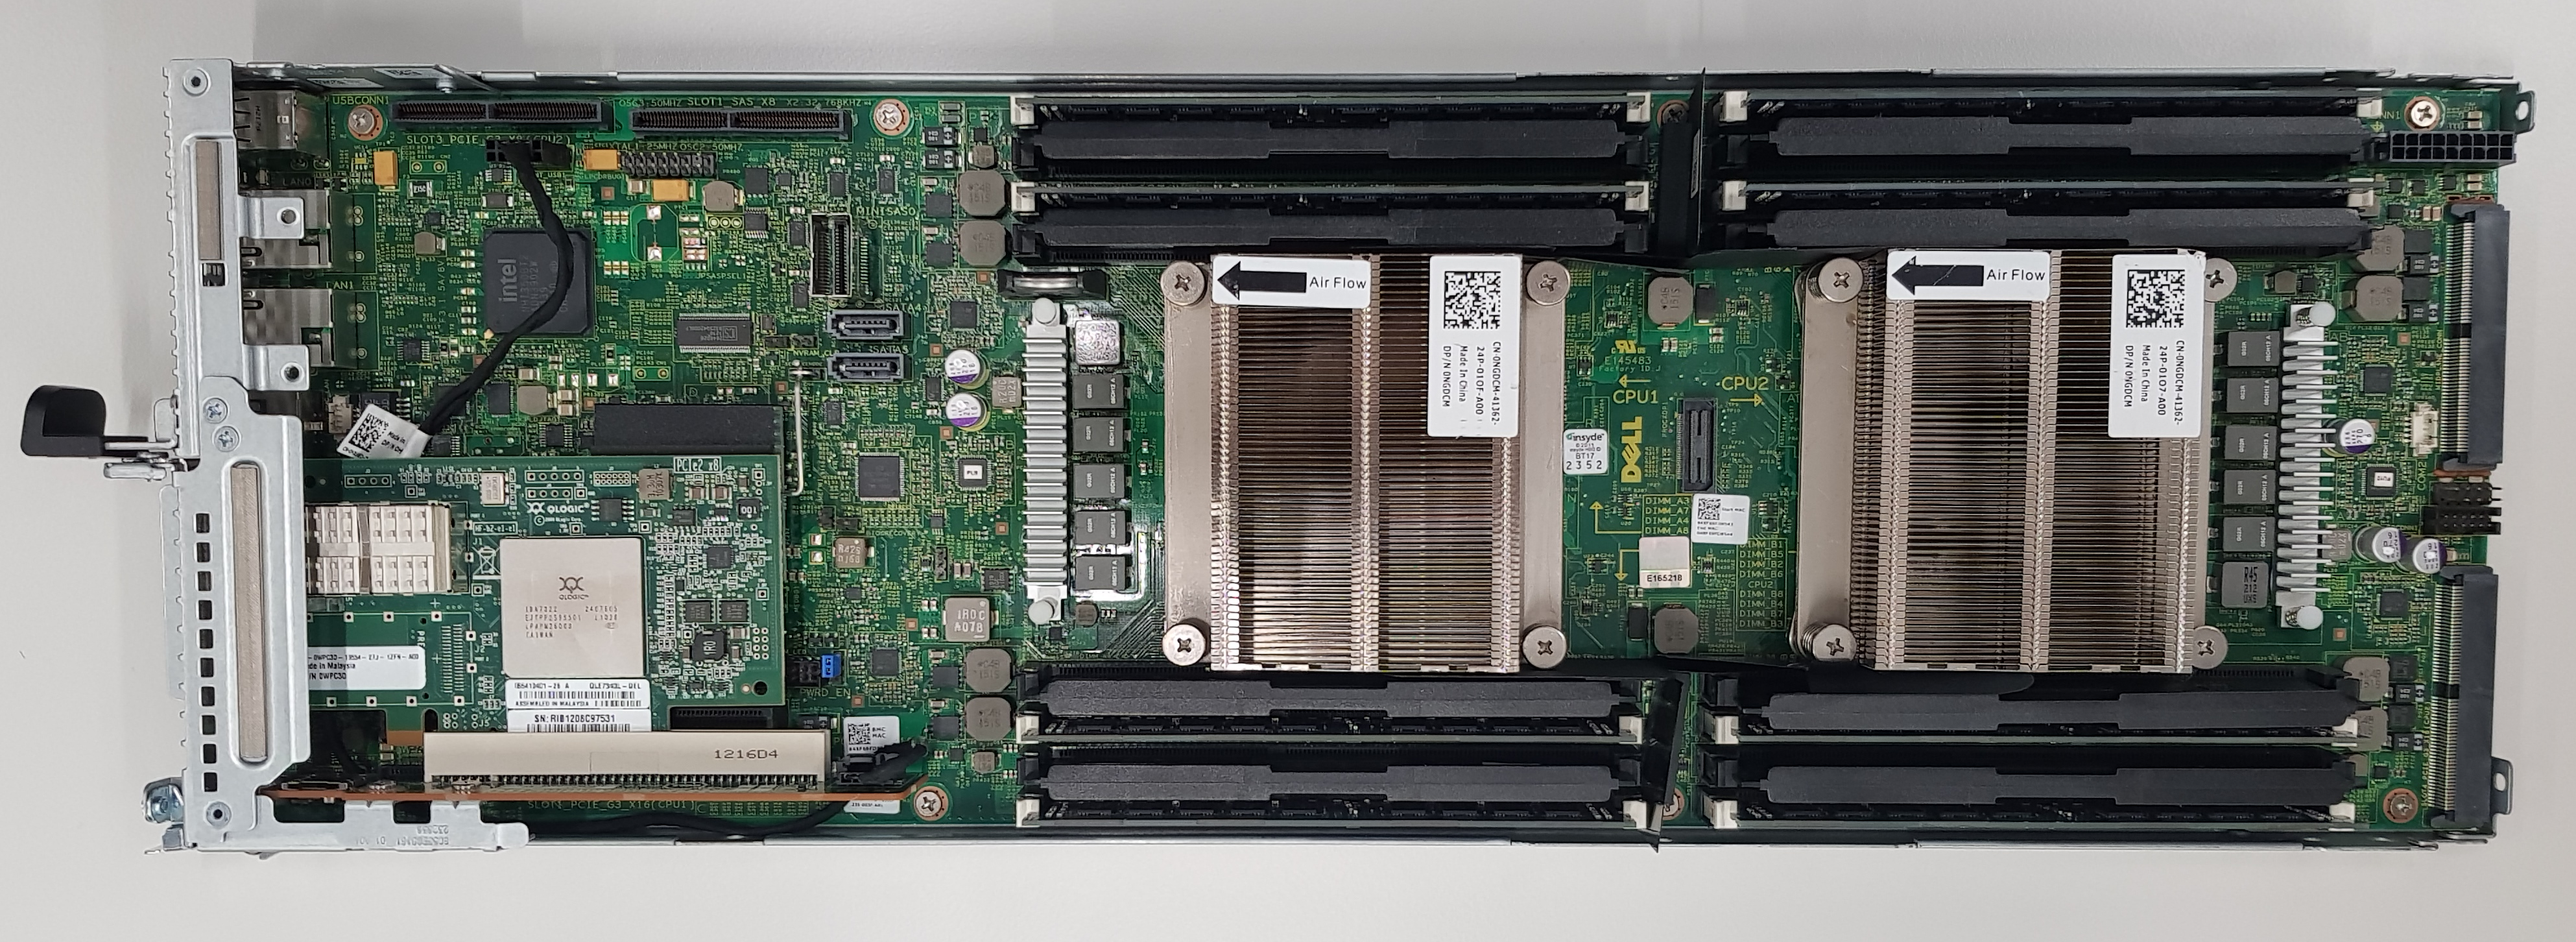
\includegraphics[height=4cm]{Day0/images/bellatrix-node.jpg}}
\end{center}
\end{frame}

\begin{frame}[containsverbatim]
\frametitle{Some important values}
\begin{itemize}
	\item{\textbf{CPU performance} measured in FLOPS (Floating Point Operations Per Second).}
	\item{\textbf{Memory bandwidth} in Bytes per second}
	\item{\textbf{Memory latency} in seconds}
\end{itemize}
It is usual to give the \textbf{peak} values (never reachable) defined by :
\begin{itemize}
	\item{\textbf{Peak CPU performance =} CPU Frequency \textbf{X} Number of Operations per clock cycle \textbf{X} size of the largest vector \textbf{X} number of cores }
	\item{\textbf{Memory bandwidth = } RAM Frequency \textbf{X} Number of transfers per clock cycle \textbf{X} Bus width \textbf{X} number of interfaces }
	\item{\textbf{Memory latency } depends on the size of the data. Usualy given by the constructor}
\end{itemize}
\end{frame}


\begin{frame}[containsverbatim]
\frametitle{Benchmarks to measure the values}
\begin{itemize}
	\item{\textbf{CPU performance} : HPL (LINPACK)}
	\item{\textbf{Memory bandwidth} : STREAM or PMBW }
	\item{\textbf{Memory latency} : Intel Memory Latency Checker}
\end{itemize}
\end{frame}

\begin{frame}[containsverbatim]
\frametitle{HPL (High Performance LINPACK)}
\begin{itemize}
	\item{Invented by Jack Dongarra (ORNL) in 1979}
	\item{solves a $n$ equations with $n$ unknown linear system $A x = b$ using Gauss partial pivoting}
	\item{This is the current benchmark for parallel computer. But it can be used to benchmark a single node or machine}
\end{itemize}
\end{frame}



\begin{frame}[containsverbatim]
\frametitle{HPL results}
\tiny
\begin{verbatim}
================================================================================
T/V                N    NB     P     Q               Time                 Gflops
--------------------------------------------------------------------------------
WR11C2R4       81792   192     4     4            1421.16              2.567e+02
HPL_pdgesv() start time Tue Oct 16 16:11:34 2018

HPL_pdgesv() end time   Tue Oct 16 16:35:15 2018

--VVV--VVV--VVV--VVV--VVV--VVV--VVV--VVV--VVV--VVV--VVV--VVV--VVV--VVV--VVV-
Max aggregated wall time rfact . . . :               6.67
+ Max aggregated wall time pfact . . :               4.28
+ Max aggregated wall time mxswp . . :               3.88
Max aggregated wall time update  . . :            1414.90
+ Max aggregated wall time laswp . . :             497.88
Max aggregated wall time up tr sv  . :               0.92
--------------------------------------------------------------------------------
||Ax-b||_oo/(eps*(||A||_oo*||x||_oo+||b||_oo)*N)=        0.0016200 ...... PASSED
================================================================================
\end{verbatim}
\end{frame}

\begin{frame}[containsverbatim]
\frametitle{HPL results on one Fidis node (f104)}
\tiny
\begin{verbatim}
================================================================================
T/V                N    NB     P     Q               Time                 Gflops
--------------------------------------------------------------------------------
WR11C2R4       81792   192     4     4             622.06              5.864e+02
HPL_pdgesv() start time Thu Oct 18 16:32:50 2018

HPL_pdgesv() end time   Thu Oct 18 16:43:12 2018

--VVV--VVV--VVV--VVV--VVV--VVV--VVV--VVV--VVV--VVV--VVV--VVV--VVV--VVV--VVV-
Max aggregated wall time rfact . . . :               2.51
+ Max aggregated wall time pfact . . :               0.64
+ Max aggregated wall time mxswp . . :               0.27
Max aggregated wall time update  . . :             619.19
+ Max aggregated wall time laswp . . :              27.47
Max aggregated wall time up tr sv  . :               0.24
--------------------------------------------------------------------------------
||Ax-b||_oo/(eps*(||A||_oo*||x||_oo+||b||_oo)*N)=        0.0017884 ...... PASSED
================================================================================
\end{verbatim}
\end{frame}



\begin{frame}[containsverbatim]
\frametitle{Memory bandwidth example}

\begin{center}
\includegraphics[page=61,width=.9\textwidth]{Day0/images/plots-scitaspc3-p1.png}
\end{center}

\end{frame}

\begin{frame}[containsverbatim]
\frametitle{Intel Memory Latency Checker (1/3)}
\tiny
\begin{verbatim}
Intel(R) Memory Latency Checker - v3.5
Measuring idle latencies (in ns)...
		Numa node
Numa node	     0	     1	
       0	  76.2	 122.9	
       1	 123.3	  75.7	

Measuring Peak Injection Memory Bandwidths for the system
Bandwidths are in MB/sec (1 MB/sec = 1,000,000 Bytes/sec)
Using all the threads from each core if Hyper-threading is enabled
Using traffic with the following read-write ratios
ALL Reads        :	101136.4	
3:1 Reads-Writes :	93459.2	
2:1 Reads-Writes :	93216.4	
1:1 Reads-Writes :	90454.1	
Stream-triad like:	81659.8	

Measuring Memory Bandwidths between nodes within system 
Bandwidths are in MB/sec (1 MB/sec = 1,000,000 Bytes/sec)
Using all the threads from each core if Hyper-threading is enabled
Using Read-only traffic type
		Numa node
Numa node	     0	     1	
       0	50481.0	 8451.7	
       1	 8415.8	50533.1	
\end{verbatim}
\end{frame}

\begin{frame}[containsverbatim]
\frametitle{Intel Memory Latency Checker (2/3}
\tiny
\begin{verbatim}
Measuring Loaded Latencies for the system
Using all the threads from each core if Hyper-threading is enabled
Using Read-only traffic type
Inject	Latency	Bandwidth
Delay	(ns)	MB/sec
==========================
 00000	170.22	 102119.1
 00002	172.92	 102090.6
 00008	176.54	 101964.0
 00015	199.00	 100029.4
 00050	174.13	  94163.3
 00100	135.42	  60156.9
 00200	119.19	  37658.6
 00300	132.01	  27635.2
 00400	122.57	  21903.4
 00500	100.41	  18037.9
 00700	 95.57	  13667.4
 01000	 93.79	   9701.4
 01300	 90.08	   7806.2
 01700	 94.09	   6234.9
 02500	 90.04	   4575.8
 03500	 85.77	   3515.6
 05000	 88.68	   2670.1
 09000	 86.89	   1830.2
 20000	 90.07	   1203.9
\end{verbatim}
\end{frame}


\begin{frame}[containsverbatim]
\frametitle{Intel Memory Latency Checker (3/3}
\tiny
\begin{verbatim}
Measuring cache-to-cache transfer latency (in ns)...
Local Socket L2->L2 HIT  latency	30.8
Local Socket L2->L2 HITM latency	35.5
Remote Socket L2->L2 HITM latency (data address homed in writer socket)
			Reader Numa Node
Writer Numa Node     0	     1	
            0	     -	  86.4	
            1	  86.3	     -	
Remote Socket L2->L2 HITM latency (data address homed in reader socket)
			Reader Numa Node
Writer Numa Node     0	     1	
            0	     -	  86.1	
            1	  86.4	     -	
\end{verbatim}
\end{frame}




\begin{frame}[containsverbatim]
\frametitle{Roofline model}
\begin{center}
        {\includegraphics[height=5cm]{Day0/images/roofline.png}}
\end{center}
\end{frame}




%\section{Compilation}
%\subsection{Compilation remainder}

\begin{frame}
\frametitle{Compilation remainder}

\begin{itemize}
	\item understanding the different compilation phases
	\item what are {\tt Makefiles} ?
	\item what happen to the application when using the different optimization flags ? 
\end{itemize}

\end{frame}

\subsection{Back to the roots}

\begin{frame}
\frametitle{{\tt 00111001011100110111...}}

{\bf Back to the roots}

\begin{itemize}
%	\item a computer (in fact a processor or a CPU) understands nothing but {\bf ON} and {\bf OFF} (one or zero)
	\item a computer (in fact a processor or a CPU) understands nothing but {\bf ON} and {\bf OFF} ({\tt 1} or {\tt 0})
	\item There is a 4-stages process to transform a {\bf source code} from a programming language into {\it something} which is understandable by the processor (the {\bf Machine Code})
\end{itemize}

\end{frame}


\begin{frame}
\frametitle{Programming languages}

Different programming languages :

\begin{itemize}
	\item {\bf C/C++} or {\bf Fortran} are high level compiled languages
%	\item {\bf Matlab}, {\bf Python}, {\bf R} are high level interpreted languages
\end{itemize}

they are {\bf human readable} % and with a {\bf high level of abstraction}

\begin{itemize}
	\item The {\bf assembly language} (depending on the CPU) is a {\bf low level language}
\end{itemize}

difficult to read. It calls only CPU instructions like a LOAD, a jump or a numerical operation.

\begin{itemize}
	\item the {\bf machine code} (depending on the CPU) is the only {\bf language understandable by the processor}
\end{itemize}

\end{frame}

\begin{frame}
\frametitle{Compilation}
\begin{alertblock}{Question}
How to produce machine code out of high-level language ? For instance from a {\tt C} source code ?
\end{alertblock}
\end{frame}

\begin{frame}
\frametitle{Punch cards}
\begin{center}
{\includegraphics[width=11cm]{Day2/images/punch-card.jpg}}
\end{center}
\end{frame}

\begin{frame}
\frametitle{Modern days : with a compiler}
\begin{center}
{% Slide 34
\begin{tikzpicture}

\node[stage] (Preproc) at (0,0) {\stagename{Preprocessor} \texttt{gcc -E file.c -o file.i}};
\node[stage] (Compiler) at (0,-2) {\stagename{Compiler} \texttt{gcc -S file.i -o file.s}};
\node[stage] (Assembler) at (0,-4) {\stagename{Assembler} \texttt{gcc -c file.s -o file.o}};
\node[stage] (Linker) at (0,-6) {\stagename{Linker} \texttt{gcc file.o -lexample -o file}};

\node[stage highlight, right of = Assembler, yshift = -1cm, xshift = 5cm, minimum width = 4cm] (Lib) {\stagename{External library} libexample.so};


\draw[->] (Preproc) -- (Compiler);
\draw[->] (Compiler) -- (Assembler);
\draw[->] (Assembler) -- (Linker);
\draw[->, dashed] (Lib.west) -- (Linker.east);

\end{tikzpicture}
}
\end{center}
\end{frame}


\begin{frame}[containsverbatim]
\frametitle{Example with a C source}
\begin{lstlisting}[language=C,frame=lines]
#include <stdio.h>
#include <stdlib.h>
#define up 10
int main() {
   int i,n;
   n = 0;
   for (i = 0; i < up; i++){
      n = n + 1;
   }
   return 0;
}
\end{lstlisting}

\url{https://gcc.godbolt.org/}

\end{frame}


\begin{frame}[containsverbatim]
\frametitle{Preprocessor ({\tt gcc -E})}
\begin{verbatim}
(...)
# 1 "/usr/include/x86_64-linux-gnu/bits/stdlib-float.h" 1 3 4
# 956 "/usr/include/stdlib.h" 2 3 4
# 968 "/usr/include/stdlib.h" 3 4

# 3 "very-simple.c" 2

int main() {
 int i,n;
 n = 0;
 for (i = 0;i < 10; i++){
  n = n + 1;
 }
 return 0;
}
\end{verbatim}
\end{frame}


\begin{frame}[containsverbatim]
\frametitle{Compiler ({\tt gcc -S})}
\begin{verbatim}
main:
.LFB2:
      pushq     %rbp
      movq      %rsp, %rbp
      movl      $0, -8(%rbp)
      movl      $0, -4(%rbp)
      jmp       .L2
.L3:
      addl      $1, -8(%rbp)
      addl      $1, -4(%rbp)
.L2:
      cmpl      $9, -4(%rbp)
      jle       .L3
      movl      $0, %eax
      popq      %rbp
      ret
\end{verbatim}
\end{frame}



\begin{frame}[containsverbatim]
\frametitle{Assembler ({\tt gcc -c})}
\begin{verbatim}
   0:	55                   	push   %rbp
   1:	48 89 e5             	mov    %rsp,%rbp
   4:	c7 45 f8 00 00 00 00 	movl   $0x0,-0x8(%rbp)
   b:	c7 45 fc 00 00 00 00 	movl   $0x0,-0x4(%rbp)
  12:	eb 08                	jmp    1c <main+0x1c>
  14:	83 45 f8 01          	addl   $0x1,-0x8(%rbp)
  18:	83 45 fc 01          	addl   $0x1,-0x4(%rbp)
  1c:	83 7d fc 09          	cmpl   $0x9,-0x4(%rbp)
  20:	7e f2                	jle    14 <main+0x14>
  22:	b8 00 00 00 00       	mov    $0x0,%eax
  27:	5d                   	pop    %rbp
  28:	c3                   	retq   
\end{verbatim}
(using {\tt objdump -d file.o})
\end{frame}


\begin{frame}[containsverbatim]
\frametitle{Linker ({\tt gcc -o})}
\begin{alertblock}{}
This last stage produces the actual executable (by linking against external libraries if required)
\end{alertblock}
\end{frame}


\begin{frame}[containsverbatim]
\frametitle{All stages in one command}

\begin{itemize}
	\item In real life, it is very unusual that one go through all the stages separatly.
	\item The two main phases are {\bf compilation} ({\tt gcc -c}) and {\bf linking} ({\tt gcc -o})
\end{itemize}

\begin{verbatim}
vkeller@deneb1:~]$ gcc -c file1.c -o file1.o
vkeller@deneb1:~]$ gcc -c file2.c -o file2.o
vkeller@deneb1:~]$ gcc file1.o file2.o -o app.exe
vkeller@deneb1:~]$ ./app.exe
\end{verbatim}

\begin{itemize}
	\item or both at once :
\end{itemize}

\begin{verbatim}
vkeller@deneb1:~]$ gcc file1.c file2.c -o app.exe
vkeller@deneb1:~]$ ./app.exe
\end{verbatim}
\end{frame}

\begin{frame}
\frametitle{But ...}

\begin{itemize}
	\item complexity whith multiple files
	\item dependencies
	\item need for a more complex tool : {\tt Makefiles} !
\end{itemize}
\end{frame}


\subsection{Makefile}

\begin{frame}
\frametitle{About Makefiles}

\begin{itemize}
	\item a {\tt Makefile} is nothing but a {\bf recipe} on how to produce an executable
		\begin{itemize}
			\item what to compile ?
			\item how to compile ?
			\item what to link ?
			\item how to link ?
		\end{itemize}
	\item useful for large projects or for testing purpose
	\item full (re)usage of {\tt variables}
	\item The usual name is {\tt Makefile} or {\tt makefile} or specified when calling {\tt make -f special.makefile}
\end{itemize}
\end{frame}

\begin{frame}[containsverbatim]
\frametitle{What is contained in a Makefile ?}
As an example
\begin{itemize}
	\item a source file {\tt poisson.c} to compile
	\item you want to produce two executable versions : 
	\begin{itemize}
		\item non-optimized with debug information
		\item optimized 
	\end{itemize}
	\item with the GNU compiler
\end{itemize}

\begin{verbatim}
gcc -O0 -g poisson.c -lm -o p-gcc-debug.exe
gcc -O3 -ftree-vectorize poisson.c -lm -o p-gcc-optim.exe
\end{verbatim}
\end{frame}

\begin{frame}[containsverbatim]
\frametitle{What is contained in a Makefile ?}
\begin{verbatim}
CC       = gcc
CFLAGS   = -O3 -ftree-vectorize
LDFLAGS  = -lm

all: p-gcc-optim.exe

.o.c: 
     $(CC) -c $(CFLAGS) $(OBJ) $<
OBJ = poisson.o

p-gcc-optim.exe: 
     $(CC) $(LDFLAGS) $(OBJ) -o $@

clean:
     rm -f *.o p-gcc-optim.exe
\end{verbatim}
\end{frame}

\begin{frame}[containsverbatim]
\frametitle{How to use the Makefile ?}

to get the optimized version :
\begin{verbatim}
make
\end{verbatim}

to get the non-optimized with debug information version :
\begin{verbatim}
make CFLAGS="-O0 -g"
\end{verbatim}

Optimized version with the Intel compiler ?
\begin{verbatim}
make CC=icc CFLAGS="-O3 -xHost" LDFLAGS=""
\end{verbatim}

or by editing the variables {\tt CC}, {\tt CFLAGS} and {\tt LDFLAGS} in the Makefile.

\end{frame}


\subsection{Optimization flags}


\begin{frame}
\frametitle{Compiler optimization}

\begin{itemize}
	\item Different levels of optimization
	\begin{itemize}
		\item instructions level
		\item datatype level
		\item global level (inter-procedural optimization or ''IPO'')
		\item loops level
		\item machine code optimization
	\end{itemize}
	\item it is possible to optimize at each level
	\item {\bf Optimization by compiler can lead to semantic changes} thus wrong results ! 
\end{itemize}

\end{frame}


\begin{frame}
\frametitle{Compiler optimization}

\begin{itemize}
	\item {\tt gcc -O0} no optimization
	\item {\tt gcc -O1} ''the compiler tries to reduce code size and execution time''
	\item {\tt gcc -O2} ''performs nearly all supported optimizations that do not involve a space-speed tradeoff''
	\item {\tt gcc -O3} ''optimize yet more. It is -O2 plus others''. Warning: this can change the code semantics.
	\item {\tt gcc -Ofast} ''Disregard strict standards compliance.''
	\item {\tt gcc -ftree-vectorize} ''perform vectorization on trees enables all -O3 optimizations plus -ffast-math''
\end{itemize}

\end{frame}






%\input{Day2/compilation-simple.tex}

%\section{Debug - Profile - Optimize - (Parallelize)}
%\subsection{Debugging-Profiling-Optimization-Parallelization}

\begin{frame}[containsverbatim]
	\frametitle{SDLC}
%	\begin{figure}[ht!]
%	\centering
	\includegraphics[width=85mm]{Day1/images/SDLC.jpg}
%	\end{figure}
\end{frame}



\begin{frame}
	\frametitle{Before you start your parallel implementation}

	\begin{itemize}
	\item {\bf You have no serial code : } design your application in a parallel way from scratch
	\item {\bf You have a serial code :} follow a Debugging-Profiling-Optimization cycle before any parallelization
	\end{itemize}
\end{frame}

\subsubsection{Debugging}

\begin{frame}
	\frametitle{Debugging ?}

	\begin{itemize}
	\item Find and correct bugs within an application
	\item Bugs can be of various nature : division by zero, buffer overflow, null pointer, infinite loops, etc.. 
	\item The compiler is (very) rarely able to recognize a bug at compilation time and the error is (very) rarely explicit regarding the bug ("syntax error")
	\item Use standard tools like {\tt gdb} 
	\item A multi-threaded code can be tricky to debug (race conditions, deadlocks, etc..)
	\item (Complex) tools exist for parallel debug : {\tt Totalview}, {\tt Alinea DDT} or recently {\tt Eclipse PTP}
	\end{itemize}

\end{frame}


\subsubsection{Profiling}

\begin{frame}
	\frametitle{Profiling ?}

Where do I spend most of the time ? 

	\begin{itemize}
	\item (good) using tools like {\tt gprof} or {\tt Intel Amplifier}
	\item (bad) ``by hand'' using timings and {\tt printf}'s
	\end{itemize}
\end{frame}

\begin{frame}
	\frametitle{Profiling ?}

What should be profiled ?

	\begin{itemize}
	\item TTS (Time To Solution)
	\item best usage of resources (storage, memory, etc..)
	\item behavior of the application to scale
	\item ...
	\end{itemize}
\end{frame}



\begin{frame}[containsverbatim]
	\frametitle{Profiling : an example with gprof}

	\begin{itemize}
	\item {{\bf MiniFE as test application} 
		\begin{itemize}
			\item 3D implicit finite-elements on an unstructured mesh
			\item mini-application written in C++
			\item \url{http://www.mantevo.org}
		\end{itemize}
	}
	\item compile with {\tt -pg -g -O3 -ftree-vectorize}
	\item run it. It should produce a {\tt gmon.out} file
	\item then profile it {\tt gprof miniFE.x}
	\end{itemize}
\end{frame}


\begin{frame}[containsverbatim]
	\frametitle{Profiling : an example with gprof}

Size : ($128~x~128~x~128$)

	\begin{Verbatim}[fontsize=\tiny]
Flat profile:

Each sample counts as 0.01 seconds.
  %   cumulative   self              self     total           
 time   seconds   seconds    calls   s/call   s/call  name    
 62.15      2.61     2.61        1     2.61     2.61  void miniFE::cg_solve
  8.57      2.97     0.36        2     0.18     0.18  void miniFE::impose_dirichlet
  5.71      3.21     0.24  7471812     0.00     0.00  int miniFE::find_row_for_id
  5.71      3.45     0.24   274625     0.00     0.00  void miniFE::Hex8::diffusionMatrix_symm
  4.76      3.65     0.20   274625     0.00     0.00  void miniFE::sum_in_symm_elem_matrix
  2.62      3.76     0.11  2197000     0.00     0.00  void miniFE::Hex8::gradients_and_invJ_and_detJ
  1.90      3.84     0.08   274625     0.00     0.00  void miniFE::get_elem_nodes_and_coords
  1.90      3.92     0.08        1     0.08     0.08  int miniFE::verify_solution
  1.67      3.99     0.07  2197000     0.00     0.00  void miniFE::Hex8::gradients_and_detJ
  0.95      4.03     0.04   274625     0.00     0.00  void miniFE::Hex8::sourceVector
  0.95      4.07     0.04        1     0.04     0.04  void miniFE::make_local_matrix
  0.71      4.10     0.03        1     0.03     0.03  std::vector::_M_fill_insert
  0.71      4.13     0.03  1649773     0.00     0.00  miniFE::mytimer()
  0.71      4.16     0.03        1     0.03     0.31  int miniFE::generate_matrix_structure
  0.48      4.18     0.02        1     0.02     0.03  void miniFE::create_map_id_to_row
  0.24      4.19     0.01        8     0.00     0.00  void miniFE::get_ids
  0.24      4.20     0.01        1     0.01     0.27  void miniFE::init_matrix
  0.00      4.20     0.00   270400     0.00     0.00  void sort_if_needed
  0.00      4.20     0.00    33282     0.00     0.00  std::_Rb_tree

...
	\end{Verbatim}
\end{frame}


\begin{frame}
	\frametitle{Profiling : an example with gprof}

What do we learn ?

	\begin{itemize}
	\item 62.15 \% of the time is spent in the solver (Conjugate Gradient)
	\item 8.57 \% is spent in imposing the boundary conditions
	\item etc..
	\item with that specific problem size ($128~x~128~x~128$). Is that similar with a larger/smaller one ?
	\end{itemize}
\end{frame}


\begin{frame}[containsverbatim]
	\frametitle{Profiling : an example with gprof}

Smaller ($16~x~16~x~16$)

	\begin{Verbatim}[fontsize=\tiny]
Flat profile:

Each sample counts as 0.01 seconds.
  %   cumulative   self              self     total           
 time   seconds   seconds    calls  ms/call  ms/call  name    
100.01      0.01     0.01        1    10.00    10.00  void miniFE::cg_solve
  0.00      0.01     0.00    18605     0.00     0.00  int miniFE::find_row_for_id
  0.00      0.01     0.00     5832     0.00     0.00  void miniFE::Hex8::gradients_and_detJ
  0.00      0.01     0.00     5832     0.00     0.00  void miniFE::Hex8::gradients_and_invJ_and_detJ
  0.00      0.01     0.00     4907     0.00     0.00  miniFE::mytimer()
  0.00      0.01     0.00      729     0.00     0.00  void sort_if_needed
  0.00      0.01     0.00      729     0.00     0.00  void miniFE::sum_in_symm_elem_matrix
  0.00      0.01     0.00      729     0.00     0.00  void miniFE::get_elem_nodes_and_coords
  0.00      0.01     0.00      729     0.00     0.00  void miniFE::Hex8::sourceVector<double>
  0.00      0.01     0.00      729     0.00     0.00  void miniFE::Hex8::diffusionMatrix_symm
  0.00      0.01     0.00      578     0.00     0.00  std::_Rb_tree<int, std::pair
  0.00      0.01     0.00      300     0.00     0.00  std::_Rb_tree<int, int, std::_Identity
  0.00      0.01     0.00      271     0.00     0.00  std::_Rb_tree<int, std::pair
  0.00      0.01     0.00      153     0.00     0.00  add_timestring_to_yaml
  0.00      0.01     0.00       52     0.00     0.00  void miniFE::exchange_externals
  0.00      0.01     0.00       26     0.00     0.00  std::vector<int, std::allocator
  0.00      0.01     0.00       25     0.00     0.00  miniFE::TypeTraits<miniFE::Vector

...
	\end{Verbatim}
\end{frame}


\begin{frame}[containsverbatim]
	\frametitle{Profiling : an example with gprof}

Larger ($512~x~512~x~512$)

	\begin{Verbatim}[fontsize=\tiny]
Flat profile:

Each sample counts as 0.01 seconds.
  %   cumulative   self              self     total           
 time   seconds   seconds    calls   s/call   s/call  name    
 63.70    228.52   228.52        1   228.52   228.87  void miniFE::cg_solve
 11.96    271.43    42.91 471862020     0.00     0.00  int miniFE::find_row_for_id
  4.87    288.90    17.47        2     8.74     8.74  void miniFE::impose_dirichlet
  4.04    303.38    14.48 16974593     0.00     0.00  void miniFE::Hex8::diffusionMatrix_symm
  3.48    315.87    12.49 16974593     0.00     0.00  void miniFE::sum_in_symm_elem_matrix
  3.29    327.68    11.81 16974593     0.00     0.00  void miniFE::get_elem_nodes_and_coords
  1.96    334.72     7.04 135796744     0.00     0.00  void miniFE::Hex8::gradients_and_invJ_and_detJ
  1.74    340.96     6.24        1     6.24     6.24  int miniFE::verify_solution
  1.29    345.60     4.64 135796744     0.00     0.00  void miniFE::Hex8::gradients_and_detJ
  0.82    348.54     2.94 16974593     0.00     0.00  void miniFE::Hex8::sourceVector
  0.64    350.83     2.29        1     2.29    45.48  void miniFE::init_matrix
  0.43    352.36     1.53        1     1.53     1.53  std::vector
  0.42    353.88     1.52        1     1.52     1.70  void miniFE::make_local_matrix
  0.40    355.31     1.43        1     1.43    48.45  int miniFE::generate_matrix_structure
  0.35    356.55     1.24 101849581     0.00     0.00  miniFE::mytimer()
  0.16    357.14     0.59        1     0.59    55.23  void miniFE::perform_element_loop
  0.11    357.55     0.41        8     0.05     0.05  void miniFE::get_ids
  0.09    357.88     0.33      201     0.00     0.00  void miniFE::exchange_externals
  0.08    358.18     0.30 16908544     0.00     0.00  void sort_if_needed
  0.05    358.35     0.17        1     0.17     0.66  void miniFE::create_map_id_to_row

...
	\end{Verbatim}
\end{frame}

\begin{frame}
	\frametitle{Profiling : an example with gprof}

Some tricks

	\begin{itemize}
	\item profile a code {\bf without bugs}
	\item choose the right size of the problem to profile (not too small, not too large)
	\item concentrate the optimization phase to the most consuming parts
	\item if the profile is not explicit, try to split the code by refactoring it into smaller functions calls
	\item take a tour of the different {\tt gprof} options
	\item {\tt gprof} works with parallel codes (OpenMP, MPI, hybrid)
	\end{itemize}
\end{frame}

\begin{frame}[containsverbatim]
	\frametitle{Profiling : with Intel Amplifier (General)}
%	\begin{figure}[ht!]
%	\centering
	\includegraphics[width=115mm]{Day1/images/Amplifier1.jpg}
%	\end{figure}
\end{frame}

\begin{frame}[containsverbatim]
	\frametitle{Profiling : with Intel Amplifier (HW counters)}
%	\begin{figure}[ht!]
%	\centering
	\includegraphics[width=115mm]{Day1/images/Amplifier2.jpg}
%	\end{figure}
\end{frame}

\begin{frame}[containsverbatim]
	\frametitle{Profiling : with Intel Amplifier (Bandwidth)}
%	\begin{figure}[ht!]
%	\centering
	\includegraphics[width=115mm]{Day1/images/Amplifier3.jpg}
%	\end{figure}
\end{frame}

\begin{frame}
	\frametitle{Profiling : with Intel Amplifier}

What do we learn ?

	\begin{itemize}
	\item the Conjugate Gradient solver ({\tt cg$\_$solve}) is the most consuming part
	\item this is due to the memory bandwidth (read from memory) limit (measured : 10.65 GB/s peak : 17.1 GB/s = DDR4-2133, STREAM : 11.8 GB/s)
	\item CPI (Clockticks per Instructions Retired) is good (0.65) : the latency is {\it probably} not a problem (cache misses, I/O or other bottlenecks)
	\end{itemize}
\end{frame}

\subsubsection{Optimization}

\begin{frame}
	\frametitle{Optimization ?}

	By order of complexity :

	\begin{enumerate}
	\item compiler and linker flags
	\item optimized external libraries
	\item ``handmade'' refactoring (loop reordering, usage of intrinsics, memory alignment, etc.. )
	\item algorithmic changes
	\end{enumerate}
\end{frame}

%\begin{frame}
%	\frametitle{Optimization : how to compare ?}
%
%	\begin{itemize}
%	\item 
%	\item 
%	\item 
%	\end{itemize}
%
%\end{frame}

\begin{frame}
	\frametitle{Optimization : when to stop ?}

Empirical ''80-20 law'' or ''The Pareto law'' : roughly 80 \% of the time is spent in 20 \% of the code

	\begin{itemize}
	\item concentrate on these 20 \% of the code
	\end{itemize}

Example with MiniFE : 80 \% of the time is spent in the solver (63), the boundary conditions (8) and reordering (5).

\end{frame}



\subsubsection{Parallelization}

\begin{frame}
	\frametitle{Parallelization ?}

Only when your sequential code has {\bf no bug} and is {\bf optimized}.

	\begin{enumerate}
	\item Is it worth to parallelize my code ? Does my algorithm scale ?
	\item Performance prediction ?
	\item Timing diagram ?
	\item Bottlenecks ? 
	\item Which parallel paradigm should I chose ? What is the target architecture (SMP, cluster, GPU, hybrid, etc..) ? 
	\end{enumerate}
\end{frame}




\subsection{A few words on high performance}


\begin{frame}
\frametitle{Parallelization of an unoptimized code}
%\framesubtitle{(... or parallelization of a non-appropriate algorithm)}

\begin{columns}
%\begin{column}[l]{7cm}
\begin{column}{7cm}
Back in 1991, David H. Bailey from Lawrence Berkeley National Laboratory released a famous paper in the Supercomputing Review: \textit{``Twelve Ways to Fool the Masses When Giving Performance Results on Parallel Computers''}.

\begin{block}{}
Number 6 was: \textit{Compare your results against scalar, unoptimized code on Crays.}
\end{block}

\end{column}
\begin{column}[c]{3cm}
{\includegraphics[height=5.3cm]{Day1/images/dhb.jpg}}
\end{column}
\end{columns}

\end{frame}


\subsubsection{The choice of the (right) compiler}

\begin{frame}[containsverbatim]
\frametitle{The compiler issue}
\label{compilerissue}
\begin{block}{}
The choice of the compiler is \textbf{very} important. Different version can lead to different performance on the same code.
\end{block}

\begin{lstlisting}[language=C,frame=lines]
      for (i=0;i<N;i++){
         for (j=0;j<N;j++){
            for (k=0;k<N;k++){
               C[i][j]=C[i][j] + A[i][k]*B[k][j];
            }
         }
      }
\end{lstlisting}

\begin{block}{}
We change the loop order and the compiler version: \texttt{i-j-k}, \texttt{i-k-j}, \texttt{j-i-k}, \texttt{j-k-i}, \texttt{k-i-j}, \texttt{k-j-i} and the two compilers: \texttt{gcc-4.8.2}, \texttt{icc 15}.
\end{block}

\end{frame}

\begin{frame}[containsverbatim]
\frametitle{\texttt{gcc} version 4.8.2, N=2000}

\verb+gcc -O3 -ftree-vectorize dgemm.c -lgsl + \\
\verb+    -lblas -lm -o dgemm+

%\begin{verbatim}
%  ijk    8000000000.00000     83.4875031      [MF/s]
%  ikj    8000000000.00000     1384.72632      [MF/s]
%  jik    8000000000.00000     83.6547699      [MF/s]
%  jki    8000000000.00000     191.552567      [MF/s]
%  kij    8000000000.00000     1517.48328      [MF/s]
%  kji    8000000000.00000     183.618088      [MF/s]
%  MKL    8000000000.00000     10047.3174      [MF/s]
%\end{verbatim}

\begin{verbatim}
  ijk         0.133   [GF/s]
  ikj         2.128   [GF/s]
  jik         0.132   [GF/s]
  jki         0.064   [GF/s]
  kij         1.914   [GF/s]
  kji         0.064   [GF/s]
  DGEMM OPT   10.35   [GF/s]
\end{verbatim}


\begin{block}{Remark}
``DGEMM OPT'' stands for the ATLAS library
\end{block}
\end{frame}

\begin{frame}[containsverbatim]
\frametitle{\texttt{icc} version 15, N=2000}

\verb+icc -DMKL_IN_USE -DMKL_ILP64 -openmp -I${MKLROOT}/include +\\
\verb+    -O3 -xHost dgemm.c  -L${MKLROOT}/lib/intel64 +\\
\verb+    -lmkl_intel_ilp64 -lmkl_core -lmkl_intel_thread+\\
\verb+    -lpthread -lm -o dgemm+

%\begin{verbatim}
%  ijk    8000000000.00000        6061.952      [MF/s]
%  ikj    8000000000.00000        6554.129      [MF/s]
%  jik    8000000000.00000        6001.980      [MF/s]
%  jki    8000000000.00000        6448.704      [MF/s]
%  kij    8000000000.00000        1636.432      [MF/s]
%  kji    8000000000.00000        6580.376      [MF/s]
%  MKL    8000000000.00000        10031.17      [MF/s]
%\end{verbatim}

\begin{verbatim}
  ijk         2.746   [GF/s]
  ikj         2.784   [GF/s]
  jik         2.586   [GF/s]
  jki        10.233   [GF/s]
  kij         2.747   [GF/s]
  kji         9.815   [GF/s]
  DGEMM OPT  27.593   [GF/s]
\end{verbatim}

\begin{block}{Remark}
``DGEMM OPT'' stands for the Intel Math Kernel Library (version 11.2)  on 8 cores
\end{block}
\end{frame}


\begin{frame}[containsverbatim]
	\frametitle{Optimization. Always ?}

Is it possible to optimize the following loop :

\begin{lstlisting}[language=Fortran,frame=lines]
do i=1,N
   do j=1,N
     y(i) = y(i) + alpha*A(i,j)*x(i) + beta*y(i)
   enddo
enddo
\end{lstlisting}

$y = \alpha A x + \beta y$

\end{frame}

\begin{frame}[containsverbatim]
	\frametitle{Optimization. Always ?}

%\begin{table}
\begin{center}
\begin{tabular}{|l|l|l|l|}
\hline
 \textbf{OPTIMIZATION} & \textbf{time (gcc)} & \textbf{time (icc)} & Difficulty \\
\hline
\hline
None ({\tt -O0}) & 65.4 & 74.1 & \\
\hline
Compiler ({\tt -O3}) & 38.6 & 1.73 & really easy\\
\hline
Compiler ({\tt -O3} + SIMD) & 39.34 & 2.6 & really easy\\
\hline
By hands (loop change) & 2.33 & 2.2 & can be compl.\\
\hline
External lib$^1$ & 0.72 & 0.70 & easy\\
\hline
\end{tabular}
\end{center}
%\caption{\texttt{N=40000}, time is in seconds. $^1$  call to dgemv() in libblas}
\texttt{N=40000}, time is in seconds. $^1$  call to dgemv() in libblas
%\end{table}

\end{frame}


\begin{frame}
	\frametitle{Performance}

{\bf Flop} (Floating Point Operations per Second)

	\begin{itemize}
	\item MFlops = MF = MF/s (MegaFlops), GFlops = GF = GF/s (GigaFlops), etc ..
	\item How to measure the Flops ?
		\begin{itemize}
			\item by hand (theoretical number of operations devided by the running time)
			\item with external tools (all based on hardware counters) : PAPI, Tau, likwid, Intel Amplxe, etc..
		\end{itemize}
	\end{itemize}

{\bf Memory} Memory Bandwidth and Memory latency

	\begin{itemize}
	\item Bandwidth in Bytes per second, latency in seconds (micro-second)
	\item How to measure memory characteristics
		\begin{itemize}
			\item by hand (theoretical number of accesses devided by the running time)
			\item with external tools (all based on hardware counters) : PAPI, Tau, Intel Amplxe, etc..
		\end{itemize}
	\end{itemize}
\end{frame}


\begin{frame}[containsverbatim]
	\frametitle{Performance example}

\begin{lstlisting}[language=C,frame=lines]
   struct timeval t;
   double t1 = gettimeoftheday(&t,0);
      for (i=0;i<N;i++){
         for (j=0;j<N;j++){
            for (k=0;k<N;k++){
               C[i][j]=C[i][j] + A[i][k]*B[k][j];
            }
         }
      }
   double t2 = gettimeoftheday(&t,0);
   double mflops = 2.0*pow(N,3) / (t2-t1) / 1.0E6 ;
\end{lstlisting}

$2 N^3$ operations

\end{frame}




%\section{Theory of parallel computing}
%
% ===============================================================================================
% ===============================================================================================
% INTRODUCTION
% 
% Small introduction tale : how to make lots of sandwiches ?
%
% ===============================================================================================
% ===============================================================================================

\subsection{Introduction}

\begin{frame}[containsverbatim]
\frametitle{}
\begin{center}
\textbf{Let's go PARALLEL !!}
\end{center}
\end{frame}

\begin{frame}[containsverbatim]
\frametitle{Introductory tale}
\begin{center}
        {\includegraphics[height=2.5cm]{Day0/images/gateau.png}}
\end{center}
\begin{center}
Next wednesday afternoon, it's Charlotte's 10$^{th}$ birthday party ! She decides to invite 20 friends.
\end{center}
\end{frame}

\begin{frame}[containsverbatim]
\frametitle{Introductory tale}
\begin{center}
        {\includegraphics[height=2.5cm]{Day0/images/sandwich.jpg}}
\end{center}
\begin{center}
... Mrs. Smith -- her mother -- will not cook special things. All the family will prepare sandwiches for Charlotte's friends. Daddy Smith and Charlotte's brother -- Mike -- too... 
\end{center}
\end{frame}


\begin{frame}[containsverbatim]
\frametitle{Introductory tale}
\begin{center}
        {\includegraphics[height=2.5cm]{Day0/images/sandwich.jpg}}
\end{center}
\begin{center}
... Mrs. Smith knows how to make a sandwich for many years. Four steps of approximatively the same duration (1 unit of time) are required :
\begin{enumerate}
	\item{\textbf{cut the bread in two halves}}
	\item{\textbf{spread the butter on the bread}}
	\item{\textbf{add a piece of ham/cheese, a few pickles and some mustard }}
	\item{\textbf{close the sandwich carefully and put it on a tray}}
\end{enumerate}
\end{center}

\end{frame}


\begin{frame}[containsverbatim]
\frametitle{Introductory tale}
\begin{center}
        {\includegraphics[height=2.5cm]{Day0/images/interrogation.png}}
\end{center}
\begin{center}
... how the family could proceed to produce 20 sandwiches in the more efficient manner ...
\end{center}

\end{frame}



\begin{frame}[containsverbatim]
\frametitle{Introductory tale}
\begin{center}
        {\includegraphics[height=2.5cm]{Day0/images/oldschool.jpg}}
\end{center}
\begin{center}
... old-school fashion ? Mrs. Smith does it all alone while Mr. Smith and kids watch TV ? 
\end{center}
\begin{center}
\begin{itemize}
	\item{\textbf{Pros: }
		\begin{itemize}
			\item{Mrs. Smith does it well without having to explain to non-professionals}
		\end{itemize}
	}
	\item{\textbf{Cons: }
		\begin{itemize}
			\item{What happens if Charlotte decides to invite the whole school to her birthday party ?}
		\end{itemize}
	}
\end{itemize}
\textbf{Time to make 20 sandwiches = 80 units of time}
\end{center}
\end{frame}


\begin{frame}[containsverbatim]
\frametitle{Introductory tale}
\begin{center}
        {\includegraphics[height=2.5cm]{Day0/images/ford.jpg}}
\end{center}
\begin{center}
... 1923 Ford T mode ? Mrs Smith cuts the bread, then Mr. Smith spread the butter while Mrs. Smith cuts a new bread, Charlotte adds ham and pickles while Mrs. cuts a bread finally Mike closes the sandwich and put it in a tray.
\end{center}
\begin{center}
\begin{itemize}
	\item{\textbf{Pros: }
		\begin{itemize}
			\item{4x more sandwiches produced when the pipeline is full}
			\item{specialized tasks, very few communications}
		\end{itemize}
	}
	\item{\textbf{Cons: }
		\begin{itemize}
			\item{each step must have the same duration}
			\item{No place for Shirley (Charlotte's best friend). 4 friends are required to produce 8x more sandwiches}
		\end{itemize}
	}
\end{itemize}
\textbf{Time to make 20 sandwiches = 23 units of time}
\end{center}
\end{frame}

\begin{frame}[containsverbatim]
\frametitle{Introductory tale}
\begin{center}
        {\includegraphics[height=2.5cm]{Day0/images/fourmis.png}}
\end{center}
\begin{center}
... totally distributed ? Mrs. \& Mr. Smith, Charlotte and Mike produce 5 sandwiches each ...
\end{center}
\begin{center}
\begin{itemize}
	\item{\textbf{Pros: }
		\begin{itemize}
			\item{Most efficient solution : number of sandwiches to produce / number of people}
		\end{itemize}
	}
	\item{\textbf{Cons: }
		\begin{itemize}
			\item{resources problem : need for 4 knives, 4 portions of butter, 4 portions of ham, etc..}
			\item{deadlocks : if only 1 knife is available, one person works when the other wait}
		\end{itemize}
	}
\end{itemize}
\textbf{Time to make 20 sandwiches = 20 units of time}
\end{center}
\end{frame}



%% ===============================================================================================
% ===============================================================================================
% PARALLELISM BASICS
%
% - Flynn
% - Amdahl's law
% - Gustaffson's law
% - speedup, etc..
% - Roofline model
%
% ===============================================================================================
% ===============================================================================================
\subsection{Parallelism basics}


\begin{frame}[containsverbatim]
\frametitle{Parallel computer}
\begin{center}
        {\includegraphics[height=7cm]{Day0/images/bellatrix2.jpg}}
\end{center}
\end{frame}

\begin{frame}[containsverbatim]
\frametitle{Parallel computer (cluster) HW components}
\begin{itemize}
	\item{\textbf{Nodes :} composed of
		\begin{itemize}
			\item{one or more \textbf{CPU} each with multiple \textbf{cores}}
			\item{\textbf{shared memory among the cores}}
			\item{\textbf{a NIC} (Networking Interface Card)}
		\end{itemize}
	}
	\item{\textbf{Interconnection network}}
	\item{\textbf{one (or more) Frontend} to access the cluster remotely}
\end{itemize}
\end{frame}

\begin{frame}[containsverbatim]
\frametitle{Parallel computer (cluster) SW components}
\begin{itemize}
	\item{\textbf{A scheduler} in order to share the resources among multiple users}
	\item{\textbf{A basic software stack} with compilers, linkers and basic parallel libraries}
	\item{\textbf{An application stack} with specific ready-to-use scientific applications}
\end{itemize}
\end{frame}



\begin{frame}[containsverbatim]
\frametitle{Vocabulary}
\begin{itemize}
	\item{\textbf{parallel computing :} data and/or task parallelism}
	\item{\textbf{supercomputing :} use of the fastest and largest machines in the world EFFICIENTLY}
	\item{\textbf{high performance computing (HPC) :} buzzword}
\end{itemize}
\end{frame}



\begin{frame}[containsverbatim]
\frametitle{Flynn taxonomy (1966)}
\begin{center}
\begin{tabular}{ l | c | c | }
	& Single instruction & Multiple instructions \\
\hline
   Single data & SISD & MISD  \\
    & Sequential processing & n/a  \\
\hline
   Multiple data & SIMD & MIMD \\
    & vector processing & distributed processing \\
\hline
 \end{tabular}
\end{center}
\end{frame}

\begin{frame}[containsverbatim]
\frametitle{Flynn taxonomy : examples}
\begin{center}
\begin{tabular}{ l | l | l | }
	& Single instruction & Multiple instructions \\
\hline
   Single data & - one core & - very rare  \\
\hline
   Multiple data & - Intel AVX512 (vectorization) & - Clusters \\
    & - GPU & \\
\hline
 \end{tabular}
\end{center}
\end{frame}


\begin{frame}[containsverbatim]
\frametitle{Parallelism ?}
Decomposition
\begin{itemize}
	\item{\textbf{on the data :} DATA PARALLELISM (SIMD)}
	\item{\textbf{on the tasks :} TASK PARALLELISM (MISD, MIMD)}
\end{itemize}

... or a mix of both !

\end{frame}

\begin{frame}[containsverbatim]
\frametitle{Data parallelism}
\begin{itemize}
	\item{loop-level parallelism}
	\item{data is distributed}
	\item{data resides on a global memory address space}
\end{itemize}
\end{frame}

\begin{frame}[containsverbatim]
\frametitle{Task parallelism}
\begin{itemize}
	\item{pipelining}
	\item{like an assembly chain}
	\item{a task is divided into a sequence of smaller tasks}
	\item{each task is executed on a specialized piece of hardware}
	\item{concurrently}
\end{itemize}
\end{frame}

\begin{frame}[containsverbatim]
\frametitle{Back to HPL (High Performance Linpack)}
\begin{itemize}
	\item{Remainder : solves $A x = b$ using Gauss partial pivoting}
	\item{We ran it on one node, but what about if we distribute the matrix A (and $x$ and $b$) over $p$ nodes ?}
	\item{Needs for a \textit{Message Passing API}. Choice is \textbf{MPI} (Message Passing Interface)}
	\item{HPL is used to rate supercomputers worldwide}
	\item{TOP500}
\end{itemize}
\end{frame}

\begin{frame}[containsverbatim]
\frametitle{HPL : parallel algorithm}
\begin{itemize}
	\item{Solves $A x = b$, where  $A \in \mathbb{R}^{n \times n}$ and $x,b \in \mathbb{R}^n$}
	\item{by computing LU factorization with row partial pivoting of the $n$ by $n+1$ coefficient matrix $[A,b]$ : $P_r[A,b] = [[L \cdot U],y]$, where $P_r,L,U \in \mathbb{R}^{n \times n}$ and $y \in \mathbb{R}^n$}
	\item{Finally : $U x = y$}
\end{itemize}
The data is ditributed onto a 2D grid (of dimension $P\times Q$) of processes using a block-cyclic scheme :
\begin{center}
\begin{tabular}{| p{0.5cm} | p{0.5cm} | p{0.5cm} | p{0.5cm} |}
\hline
$P_0$ & $P_1$ & $P_0$ & $P_1$ \\
\hline
$P_2$ & $P_3$ & $P_2$ & $P_3$ \\
\hline
$P_0$ & $P_1$ & $P_0$ & $P_1$ \\
\hline
$P_2$ & $P_3$ & $P_2$ & $P_3$ \\
\hline
\end{tabular}
\end{center}
\end{frame}




\begin{frame}[containsverbatim]
\frametitle{TOP500}
\begin{center}
        {\includegraphics[height=5cm]{Day0/images/Top500_logo.png}}
\end{center}
\end{frame}


\begin{frame}[containsverbatim]
\frametitle{TOP500 : current list (November 2019)}
\scriptsize
\begin{tabular}{| l | l | l | l | l | l | l | }
\hline
 \textbf{Rank} & \textbf{Machine} & \textbf{\# cores} & \textbf{$R_{\infty}$} & \textbf{$R_{max}$} & \textbf{Power} & \textbf{Country}\\
               &                  &                   &  in TFlop/s           & in TFlop/s         & in KW & \\
\hline
\hline
1 & Summit & 2,414,592&148,600.0 &200,794.9 & 10,096 & USA\\
\hline
2 & Sierra & 1,572,480 &94,640.0 &125,712.0 & 7,438 & USA\\
\hline
3 & Sunway & 10,649,600 &93,014.6 &125,435.9 &15,371 & China\\
 & TaihuLight &  & & & &\\
\hline
4 & Tianhe-2A & 4,981,760 &61,444.5 & 100,678.7 &18,482 & China\\
\hline
5 & Frontera & 448,448 &23,516.4 &38,745.9 &n/a& USA\\
\hline
6 &  Piz Daint & 387,872 &21,230.0 &27,154.3 &2,384& Switzerland\\
\hline
7 &  Trinity & 979,072 &20,158.7 &41,461.2 &7,578& USA\\
\hline
8 &  Al Bridging & 391,680 &19,880.0 &32,576.6 &1,649& Japan\\
\hline
9 &  SuperMUC & 305,856 &19,476.6 &26,873.9 &n/a& Germany\\
\hline
10 & Lassen & 288,288 &18,200.0 &23,047.2 &n/a& USA\\
\hline

\end{tabular}
\end{frame}




%\begin{frame}[containsverbatim]
%\frametitle{TOP500 : current list (June 2018)}
%\scriptsize
%\begin{tabular}{| l | l | l | l | l | l | }
%\hline
% \textbf{Rank} & \textbf{Machine} & \textbf{\# cores} & \textbf{$R_{\infty}$} & \textbf{$R_{max}$} & \textbf{Power} \\
%               &                  &                   &  in TFlop/s           & in TFlop/s         & in KW \\
%\hline
%\hline
%1 & Summit & 2,282,544&122,300.0 &187,659.3 & 8,806 \\
%\hline
%2 & Sunway TaihuLight & 10,649,600 &93,014.6 &125,435.9 &15,371 \\
%\hline
%3 & Sierra & 1,572,480 &71,610.0 &119,193.6 & n/a \\
%\hline
%4 & Tianhe-2A & 4,981,760 &61,444.5 & 100,678.7 &18,482 \\
%\hline
%5 &  Al Bridging & 391,680 &19,880.0 &32,576.6 &1,649\\
%\hline
%6 &  Piz Daint & 361,760 &19,590.0 &25,326.3 &2,272\\
%\hline
%7 &  Titan & 560,640 &17,590.0 &27,112.5 &8,209\\
%\hline
%8 &  Sequoia & 1,572,864 &17,173.2 &20,132.7 &7,890\\
%\hline
%9 &  Trinity & 979,968 &14,137.3 &43,902.6 &3,844\\
%\hline
%10 &  Cori & 622,336 &14,014.7 &27,880.7 &3,939\\
%\hline
%
%\end{tabular}
%\end{frame}





% ===============================================================================================
% ===============================================================================================
% PARALLEL APPLICATIONS AND ALGORITHMS
%
%
% ===============================================================================================
% ===============================================================================================
\subsection{Parallel applications and algorithms}

\begin{frame}[containsverbatim]
\frametitle{}

\begin{center}
\textbf{Theoretical analysis of a code}
\end{center}

\end{frame}


\begin{frame}[containsverbatim]
\frametitle{Performance analysis}
\textbf{Before starting parallelization : insight of the application} 
\begin{itemize}
	\item{is the algorithm/application a good candidate for parallelization ?}
	\item{Which parallelization strategy should I choose ?}
	\item{How should I partition the problem ?}
\end{itemize}
\textbf{Helps understanding and improving existing implementations}
\begin{itemize}
	\item{do the benchmark match the performance predictions ?}
	\item{which factors have most influence on the performance ?}
	\item{which HW fits most to the applications needs ?}
\end{itemize}
\end{frame}




\begin{frame}
\frametitle{Speedup and efficiency}

\[
S(p) = \frac{T_{1}}{T_{p}} \qquad E(p) = \frac{S(p)}{p}
\]

where

\begin{itemize}
	\item{\textbf{$T_1$ :} Execution time using 1 process }
	\item{\textbf{$T_p$ :} Execution time using p process }
	\item{\textbf{$S(p)$ :} Speedup of $p$ processes }
	\item{\textbf{$E(p)$ :} Parallel Efficiency }
\end{itemize}

Example :

\begin{columns}
    \begin{column}{0.47\textwidth}
\begin{tabular}{| l | l | l | l |}
\hline
 \textbf{n} & \textbf{Walltime in [s]} & \textbf{S(p)}& \textbf{E(p)} \\
\hline
\hline
1 & 24.5 & 1.0 & 1.0\\
\hline
2 & 13.4 & 1.8 & 0.9\\
\hline
4 & 6.8 & 3.6 & 0.9\\
\hline
8 & 4.0.5 & 6.1 & 0.76\\
\hline
\end{tabular}
    \end{column}
    \begin{column}{0.5\textwidth}
        \includegraphics[width=\textwidth]{Day0/images/speedup.png} 
    \end{column}
\end{columns}
\end{frame}

\begin{frame}[containsverbatim]
\frametitle{Amdahl's law}
\begin{itemize}
	\item{\textbf{Maximum achievable speedup} for an application where a fraction $f$ cannot be parallelized}
	\item{$S(p)  \leqslant  \frac{1}{f + \frac{(1-f)}{p}}$}
	\item{or $S(p)  \leqslant  \frac{p}{1 + (p-1) \cdot f}$}
	\item{$S(p)$ is always lower than $\frac{1}{f}$: $lim_{p \rightarrow \infty} S(p)  \leqslant \frac{1}{f}$}
	\item{Desirable : $f < \frac{1}{p}$}
	\item{provides an upperbound}
\end{itemize}
\end{frame}

\begin{frame}[containsverbatim]
\frametitle{Amdahl's law}
\begin{center}
        {\includegraphics[height=5cm]{Day0/images/amdahl.png}}
\end{center}
\end{frame}


\begin{frame}[containsverbatim]
\frametitle{Amdahl's law (deduce $f$)}
\begin{align} 
S_p &= \frac{1}{f + \frac{(1-f)}{p}}
\end{align}
then 
\begin{align} 
S_p \cdot f + \frac{S_p}{p} - S_p \cdot \frac{f}{p} &= 1 
\end{align}
finally :
\begin{align} 
f &= \frac{1 - \frac{S_p}{p}}{S_p - \frac{S_p}{p}} = \frac{\frac{1}{S_p} - \frac{1}{p}}{1 - \frac{1}{p}}
\end{align}
$f$ comprise communication overhead
\end{frame}

\begin{frame}
\frametitle{Amdahl and Gustafson}
\begin{exampleblock}{Observation}
Amdahl's law is an estimation for a \textbf{fixed problem size} $n$.
\end{exampleblock}
\begin{alertblock}{Problem}
If we increase the problem size, the relative sequential part can be made smaller and smaller \textit{if it is of lower complexity than the parallel part of the problem}
\end{alertblock}
\begin{alertblock}{Solution}
Take the problem size $n$ into account. This is Gustafson's law (or Gustafson's complement to Amdahl's law)
\end{alertblock}
\end{frame}


\begin{frame}[containsverbatim]
\frametitle{Gustafson's law}
$s$ is the sequential portion, $a$ is the parallel portion. The sequential ($t_s$) and parallel ($t_p$) are:

\[
t_s = s + a \cdot n \qquad t_p = s + a \cdot \frac{n}{p}
\]

then the Speedup $S_p$ is :

\begin{align} 
S_p &= \frac{t_s}{t_p} = \frac{s + a \cdot n}{s + a \cdot \frac{n}{p}} = \frac{\frac{s}{n} + a}{\frac{s}{n} + \frac{a}{p}}
\end{align}

Note $lim_{n \rightarrow \infty} S_p = p$

\end{frame}




\begin{frame}[containsverbatim]
\frametitle{Gustafson's law}
\begin{center}
        {\includegraphics[height=5cm]{Day0/images/gustafson.png}}
\end{center}
\end{frame}

\begin{frame}[containsverbatim]
\frametitle{Complexity analysis}
\begin{exampleblock}{Observation}
The speedup $S(p)$ is determined by the \textbf{computation time} and the \textbf{communication time}, function of the problem size $n$
\end{exampleblock}
\begin{exampleblock}{Communication \& computation time}
It is an overhead to the parallel execution time. It can be partially hidden by computation.
\end{exampleblock}
\begin{exampleblock}{Complexity}
Computing the \textbf{complexity} $\mathcal{O}(n,p)$ provides an insight into the parallelization potential.
\end{exampleblock}
\end{frame}

%%%%%%%%%%%%%%%%%%%%%%%%%%%%%%%%%%%%%%%%%%%%%%%%%%%%%%%%
%%%%%%%%%%%%%%%%%%%%%%%%%%%%%%%%%%%%%%%%%%%%%%%%%%%%%%%%
% FIXME : Prendre l'exemple du matrice vecteur à la place de matrice matrice
% voir page 9 : https://www3.nd.edu/~zxu2/acms60212-40212-S12/Lec-05.pdf
% plus : http://www.hpcc.unn.ru/mskurs/ENG/DOC/pp07.pdf (complexity analysis + dependencies)
%%%%%%%%%%%%%%%%%%%%%%%%%%%%%%%%%%%%%%%%%%%%%%%%%%%%%%%%
%%%%%%%%%%%%%%%%%%%%%%%%%%%%%%%%%%%%%%%%%%%%%%%%%%%%%%%%


\begin{frame}[containsverbatim]
\frametitle{Complexity analysis : example $c = A \cdot b$}
\textbf{Full $N \times N $ matrix vector multiplication with the naïve method $\mathcal{O}(N^2)$}
\begin{lstlisting}[language=C,frame=lines]
   struct timeval t;
   double t1 = gettimeoftheday(&t,0);
   for (i=0;i<N;i++){
      for (j=0;j<N;j++){
         c[i] = c[i] + A[i][j]*b[j];
      }
   }
   double t2 = gettimeoftheday(&t,0);
   double mflops = 2.*(double)N*(double)N / (t2-t1) / 1.0E6;
\end{lstlisting}
\end{frame}


\begin{frame}[containsverbatim]
\frametitle{Complexity analysis : example $c = A \cdot b$}
\textbf{Sequential algorithm :}
\begin{itemize}
	\item{\textbf{Time complexity :} $\mathcal{O}(N)$}
	\item{\textbf{Size complexity :} $\mathcal{O}(N^2)$}
\end{itemize}
\end{frame}

\begin{frame}[containsverbatim]
\frametitle{Complexity analysis : example $c = A \cdot b$}
\textbf{Parallel version}
\begin{lstlisting}[language=C,frame=lines]
   t1 = MPI_Wtime();
   MPI_Bcast(b, ndiag, MPI_FLOAT, 0, MPI_COMM_WORLD);
   MPI_Scatter(A,(nn_loc*ndiag),MPI_FLOAT,A_loc,(nn_loc*ndiag),MPI_FLOAT,0,MPI_COMM_WORLD);
   t2 = MPI_Wtime();		
   for (j=0;j<ndiag;j++){
      for (i=0;i<nn_loc;i++){
         c[i] = c[i] + A_loc[i+j*nn_loc]*b[i];
      }
   }
   t3 = MPI_Wtime();
   MPI_Gather(c,nn_loc,MPI_FLOAT,b,nn_loc,MPI_FLOAT,0,MPI_COMM_WORLD);
   t4 = MPI_Wtime();
\end{lstlisting}
\end{frame}


%\begin{frame}[containsverbatim]
%\frametitle{Complexity analysis : example $c = A \cdot b$}
%\textbf{Parallel version}
%\begin{lstlisting}[language=C,frame=lines]
%   t1 = MPI_Wtime();
%   MPI_Bcast(U, ndiag, MPI_FLOAT, 0, MPI_COMM_WORLD);
%   MPI_Scatter(A,(nn_loc*ndiag),MPI_FLOAT,A_loc,(nn_loc*ndiag),MPI_FLOAT,0,MPI_COMM_WORLD);
%   t2 = MPI_Wtime();		
%   for (j=0;j<ndiag;j++){
%      for (i=0;i<nn_loc;i++){
%         Ua[i] = Ua[i] + A_loc[i+j*nn_loc]*U[i];
%      }
%   }
%   t3 = MPI_Wtime();
%   MPI_Gather(Ua,nn_loc,MPI_FLOAT,U,nn_loc,MPI_FLOAT,0,MPI_COMM_WORLD);
%   t4 = MPI_Wtime();
%\end{lstlisting}
%\end{frame}



\begin{frame}[containsverbatim]
\frametitle{Complexity analysis : example $c = A \cdot b$}
\textbf{Parallel algorithm over $p$ processes:}
\begin{itemize}
	\item{\textbf{Computational complexity :} $\mathcal{O}(\frac{N^2}{p})$}
	\item{\textbf{Communication complexity :} $\mathcal{O}(log p + N)$}
	\item{\textbf{Overall complexity :} $\mathcal{O}(\frac{N^2}{p} + log p + N)$}
	\item{for \textit{reasonably} large $N$, latency is neglictible compared to bandwidth}
	\item{The algorithm is not scalable}
\end{itemize}
\end{frame}







\begin{frame}[containsverbatim]
\frametitle{On the importance of algorithmic analysis}
\textbf{Full $N \times N $ matrix matrix multiplication with the naïve method $\mathcal{O}(N^3)$}
\begin{lstlisting}[language=C,frame=lines]
   struct timeval t;
   double t1 = gettimeoftheday(&t,0);
      for (i=0;i<N;i++){
         for (j=0;j<N;j++){
            for (k=0;k<N;k++){
               C[i][j]=C[i][j] + A[i][k]*B[k][j];
            }
         }
      }
   double t2 = gettimeoftheday(&t,0);
   double mflops = 2.0*pow(N,3) / (t2-t1) / 1.0E6 ;
\end{lstlisting}
\end{frame}

\begin{frame}[containsverbatim]
\frametitle{On the importance of algorithmic analysis}
\begin{center}
        {\includegraphics[height=5cm]{Day0/images/dgemm-complexity.png}}
\end{center}
\end{frame}


%\begin{frame}[containsverbatim]
%\frametitle{Complexity analysis : HPL example}
%\begin{exampleblock}{Complexity}
%$\mathcal{O}(n^3)$ more specifically $\frac{2}{3} n^3 " 2 n^2 + \mathcal{O}(n)$ floating-point multiplications and additions 
%\end{exampleblock}
%
%\end{frame}




\begin{frame}[containsverbatim]
\frametitle{Task dependency graph}
\begin{center}
        {\includegraphics[height=3cm]{Day0/images/dependency.png}}
\end{center}
{\tiny Image from : Wu, Hao \& Hua, Xiayu \& Li, Zheng \& Ren, Shangping. \textit{Resource and Instance Hour Minimization for Deadline Constrained DAG Applications Using Computer Clouds}. IEEE TPDS. 2015}
\begin{itemize}
	\item{essentially a DAG (nodes = tasks, edges = dependencies)}
	\item{\textbf{critical path :} the longest path from starting task to the ending task}
	\item{\textbf{average degree of concurrency :} total amount of work devided by the critical path length}
\end{itemize}
\end{frame}




\begin{frame}[containsverbatim]
\frametitle{New bug in concurrent computing : deadlock}
\begin{center}
        {\includegraphics[height=3cm]{Day0/images/deadlock.png}}
\end{center}
\begin{itemize}
	\item{P1 holds resource R2 and requires R1}
	\item{P2 holds resource R1 and requires R2}
	\item{\textbf{deadlock !!}}
\end{itemize}
\end{frame}


\begin{frame}[containsverbatim]
\frametitle{New bug in concurrent computing : race condition}
\begin{itemize}
	\item{arise in concurrent computing when two (or more) processes depends on a sequence or timing on a shared variable}
	\item{example : $a = 0$ is a shared variable. P1 will do $a+1$ while P2 will do $a+2$ : 
		\begin{enumerate}
			\item{[P1] read $a = 0$}
			\item{[P2] read $a = 0$}
			\item{[P1] incr $a = 1$}
			\item{[P2] incr $a = 2$}
		\end{enumerate}
		}
	\item{The order can lead to different $a$ values : if 2 and 3 are interverted :
		\begin{enumerate}
			\item{[P1] read $a = 0$}
			\item{[P1] incr $a = 1$}
			\item{[P2] read $a = 1$}
			\item{[P2] incr $a = 3$}
		\end{enumerate}
	}
	\item{\textbf{race condition !!}}
\end{itemize}

\end{frame}







%\section{Parallelization with OpenMP}
%	\subsection{Introduction}


\begin{frame}
  \begin{center}
    {\includegraphics[height=2cm]{Day1/images/logo_OpenMP.png}}

    \textbf{Lecture based on specifications ver 3.1}

  \end{center}
\end{frame}

\begin{frame}
  \frametitle{Releases history, present and future}
  \begin{itemize}
  \item{October 1997: Fortran version 1.0 }
  \item{Late 1998: C/C++ version 1.0 }
  \item{June 2000: Fortran version 2.0 }
  \item{April 2002: C/C++ version 2.0 }
  \item{June 2005: Combined C/C++ and Fortran version 2.5 }
  \item{May 2008: Combined C/C++ and Fortran version  3.0}
  \item{\textbf{July 2011: Combined C/C++ and Fortran version  3.1}}
  \item{July 2013: Combined C/C++ and Fortran version 4.0 }
  \item{November 2015: Combined C/C++ and Fortran version 4.5 }
  \end{itemize}
\end{frame}

% \subsubsection{threading concepts, terminology (OpenMP, tasking, data, implementation)}

\begin{frame}
  \frametitle{Terminology}
  \begin{itemize}
  \item{\textbf{thread :} an execution entity with a stack and a static memory (\textit{threadprivate memory})}
  \item{\textbf{OpenMP thread :} a \textit{thread} managed by the OpenMP runtime}
  \item{\textbf{thread-safe routine :} a routine that can be executed concurrently}
  \item{\textbf{processor :} an HW unit on which one or more \textit{OpenMP thread} can execute}
%  \item{\textbf{device :} an implementation defined logical execution engine}
  \end{itemize}
\end{frame}

\subsubsection{Models}

\begin{frame}
  \frametitle{Execution and memory models}
  \begin{itemize}
  \item{Execution model : fork-join}
  \item{One heavy thread (process) per program (initial thread)}
  \item{leightweigt threads for parallel regions. threads are assigned to cores by the OS}
  \item{No implicit synchronization (except at the beginning and at the end of a parallel region)}
  \item{Shared Memory with shared variables}
  \item{Private Memory per thread with threadprivate variables}
  \end{itemize}
\end{frame}

\begin{frame}
  \frametitle{Memory model (simplified)}
  \begin{center}
    {\includegraphics[width=\textwidth]{Day1/images/memory-model-simplified.pdf}}
  \end{center}
\end{frame}

\begin{frame}
  \frametitle{Execution model (simplified)}
  \begin{center}
    {% Slide 72
\begin{tikzpicture}[yscale = 0.7, xscale = 0.9]

\draw[very thick, ->] (0,8.5) node[above right] {Master thread} -- (0,-1);

\pgfmathsetmacro{\forkheight}{7}

\foreach \x in {1, 2, ..., 5} {
	\draw[blue2, ->, thick] (0,{\forkheight + 0.5})
		to[out = -90, in = 180] (0.5, \forkheight)
		-- ({\x - 0.5}, \forkheight)
		to[out=0, in = 90] (\x, {\forkheight-0.5}) -- (\x, {\forkheight - 2});

	\draw[blue2, thin] (\x, {\forkheight - 2})
		to[out = -90, in = 0] ({\x - 0.5}, {\forkheight - 2.25})
		-- (0.5, {\forkheight - 2.25})
		to[out = 180, in = 90] (0, {\forkheight - 2.5});
}

\node[point, label={left:Fork}] at (0, {\forkheight + 0.5}) {};
\node[point, label={left:Join}] at (0, {\forkheight - 2.5}) {};
\node[blue2, anchor = south, yshift = 0.1cm] at (4, \forkheight) {Worker threads};

\pgfmathsetmacro{\forkheight}{2.5}

\foreach \x in {1, 2, 3} {
	\draw[blue2, ->, thick] (0,{\forkheight + 0.5})
		to[out = -90, in = 180] (0.5, \forkheight)
		-- ({\x - 0.5}, \forkheight)
		to[out=0, in = 90] (\x, {\forkheight-0.5}) -- (\x, {\forkheight - 2});

	\draw[blue2, thin] (\x, {\forkheight - 2})
		to[out = -90, in = 0] ({\x - 0.5}, {\forkheight - 2.25})
		-- (0.5, {\forkheight - 2.25})
		to[out = 180, in = 90] (0, {\forkheight - 2.5});
}

\node[blue2, anchor = south, yshift = 0.1cm] at (2, \forkheight) {Worker threads};

\node[point, label={left:Fork}] at (0, {\forkheight + 0.5}) {};
\node[point, label={left:Join}] at (0, {\forkheight - 2.5}) {};

\end{tikzpicture}
}
  \end{center}
\end{frame}

\subsubsection{Remarks}

\begin{frame}
  \frametitle{OpenMP and MPI/pthreads	}
  \begin{itemize}
  \item{\textbf{OpenMP} $\neq$ OpenMPI}
  \item{All what you can do with OpenMP can be done with MPI and/or pthreads}
    % \item{Memory issue}
  \item{easier \textbf{BUT} data coherence/consistency}
    % \item{In fact: \textbf{no} easy parallel paradigm exists}
  \end{itemize}
\end{frame}

\subsection{Directives}

\subsubsection{format \& conditional compilation}

\begin{frame}[containsverbatim]
  \frametitle{Syntax in C}
  % \begin{itemize}
  % \item{OpenMP directives are written as pragmas: \texttt{\#pragma omp}}
  % \item{Use the conditional compilation flag \texttt{\#if defined \_OPENMP} for the preprocessor}
  % \end{itemize}

  \begin{block}{}
    OpenMP directives are written as pragmas: \texttt{\#pragma omp}
  \end{block}

  \begin{block}{}
    Use the conditional compilation flag \texttt{\#if defined \_OPENMP} for the preprocessor
  \end{block}

  Compilation using the GNU gcc or Intel compiler:
\begin{verbatim}
gcc -fopenmp ex1.c -o ex1
\end{verbatim}
\end{frame}


\begin{frame}[containsverbatim]
  \frametitle{Hello World in C}

  \begin{lstlisting}[language=C++,frame=lines]
#include <stdio.h>
#include <omp.h>
int main(int argc, char *argv[]) {
   int myrank=0;
   int mysize=1;
#if defined (_OPENMP)
#pragma omp parallel default(shared) private(myrank, mysize)
{
   mysize = omp_get_num_threads();
   myrank = omp_get_thread_num();
#endif
   printf("Hello from thread %d out of %d\n", myrank, mysize);
#if defined (_OPENMP)
}
#endif
   return 0;
}
\end{lstlisting}
% (Source file: \texttt{ex1.c})
\end{frame}

\begin{frame}[containsverbatim]
  \frametitle{Syntax in Fortran 90}
  % \begin{itemize}
  % \item{OpenMP directives are written as comments: \texttt{!\$omp omp}}
  % \item{Sentinels \texttt{!\$} are authorized for conditional compilation  (preprocessor) }
  % \end{itemize}

  \begin{block}{}
    OpenMP directives are written as comments: \texttt{!\$omp omp}
  \end{block}
  \begin{block}{}
    Sentinels \texttt{!\$} are authorized for conditional compilation  (preprocessor)
  \end{block}


  Compilation using the GNU gfortran or Intel ifort compiler:
\begin{verbatim}
gfortran -fopenmp ex1.f90 -o ex1
\end{verbatim}
\end{frame}



\begin{frame}[containsverbatim]
  \frametitle{Hello World in Fortran 90}

  \begin{lstlisting}[language=Fortran,frame=lines]
program ex1
   implicit none
   integer :: myrank, mysize
!$ integer, external :: omp_get_num_threads, omp_get_thread_num
   myrank=0
   mysize=1
!$omp   parallel default(shared) private(myrank, mysize)
!$      mysize = omp_get_num_threads()
!$      myrank = omp_get_thread_num()
   print *, "Hello from thread",myrank,"out of",mysize
!$omp   end parallel
end program ex1
\end{lstlisting}
% $ This comment is just for the colors in emacs...
\end{frame}

\begin{frame}[containsverbatim]
  \frametitle{Number of concurrent threads}

  The number of threads is specified in a hardcoded way ($omp\_set\_num\_threads()$) or via an environment variable.
  \\~\\

  BASH-like shells :

\begin{verbatim}
export OMP_NUM_THREADS=4
\end{verbatim}

  CSH-like shells :

\begin{verbatim}
setenv OMP_NUM_THREADS 4
\end{verbatim}
\end{frame}


\begin{frame}[containsverbatim]
  \frametitle{Components of OpenMP}
  \begin{itemize}
  \item{Compiler directives (written as comments) that allow work sharing, synchronization and data scoping}
  \item{A runtime library (libomp.so) that contains informal, data access and synchronization directives}
  \item{Environment variables}
  \end{itemize}
\end{frame}


\subsubsection{The \texttt{parallel} construct}


\begin{frame}[containsverbatim]
  \frametitle{The \texttt{parallel} construct}

  \begin{exampleblock}{Syntax}
    This is the mother of all constructs in OpenMP. It starts a parallel execution.
    \begin{lstlisting}[language=C,frame=lines]
#pragma omp parallel [clause[[,] clause]...]
{
   structured-block
}
\end{lstlisting}
    where \textit{clause} is one of the following:
    \begin{itemize}
    \item \textbf{\texttt{if}} or \textbf{\texttt{num\_threads}} : conditional clause
    \item \textbf{\texttt{default(private | firstprivate | shared | none)}} : default data scoping
    \item \textbf{\texttt{private(\textit{list})}}, \textbf{\texttt{firstprivate(\textit{list})}}, \textbf{\texttt{shared(\textit{list})}} or \textbf{\texttt{copyin(\textit{list})}} : data scoping
    \item \textbf{\texttt{reduction(\textit{\{ operator | intrinsic\_procedure\_name \} : list})}}
    \end{itemize}
  \end{exampleblock}
\end{frame}


\begin{frame}[fragile]
  \frametitle{Example : the \texttt{if} conditional clause }

  \begin{block}{The \texttt{if} clause}
    A \texttt{if} test specifies if a parallel region must be executed in parallel or not:

\begin{verbatim}
if (n<2) then
   execute test(n) serial
else
   execute test(n) in parallel
endif
\end{verbatim}

  \end{block}

  \begin{lstlisting}[language=C,frame=lines]
#pragma omp parallel if (n>2)
   test(n);
\end{lstlisting}
\end{frame}

\begin{frame}[containsverbatim]
  \frametitle{The \texttt{if} clause [output]}

\begin{verbatim}
vkeller@mathicsepc13:~/OpenMP/exercises/C$ ./ex3
 var =       1  : Code is executed by only one thread
 Parallelized with           2 threads :            2
 Parallelized with           3 threads :            3
 Parallelized with           4 threads :            4
\end{verbatim}

\end{frame}


\begin{frame}[containsverbatim]
  \frametitle{Data scoping}
  What is data scoping ?
  \begin{itemize}
  \item{most common source of errors}
  \item{determine which variables are {\bf private} to a thread, which are {\bf shared} among all the threads}
  \item{In case of a private variable, what is its value when entering the
      parallel region {\bf firstprivate}, what is its value when leaving the
      parallel region {\bf lastprivate}}
  \item The default scope (if none are specified) is \textbf{shared}
  \item{most difficult part of OpenMP}
  \end{itemize}
\end{frame}


\begin{frame}[fragile]
  \frametitle{The data sharing-attributes \texttt{shared} and \texttt{private}}
  \begin{exampleblock}{Syntax}
These attributes determines the scope (visibility) of a single or list of variables
\begin{lstlisting}[language=C,frame=lines]
shared(list1) private(list2)
\end{lstlisting}

\begin{itemize}
\item{The \verb+private+ attribute : the data is private to each thread and non-initiatilized. Each thread has its own copy. Example : \verb+#pragma omp parallel private(i)+}
\item{The \verb+shared+ attribute : the data is shared among all the threads. It is accessible (and non-protected) by all the threads simultaneously. Example : \verb+#pragma omp parallel shared(array)+}
\end{itemize}

\end{exampleblock}

\end{frame}



\begin{frame}[containsverbatim]
\frametitle{The data sharing-attributes \texttt{firstprivate} and \texttt{lastprivate}}
\begin{exampleblock}{Syntax}
These clauses determines the attributes of the variables within a parallel region:
\begin{lstlisting}[language=C,frame=lines]
firstprivate(list1) lastprivate(list2)
\end{lstlisting}
\begin{itemize}
\item{The \texttt{firstprivate} like {\tt private} but initialized to the value before the parallel region}
\item{The \texttt{lastprivate}  like {\tt private} but the value is updated after the parallel region}
\end{itemize}
\end{exampleblock}
%\begin{alertblock}{}
%\textbf{Fortran only !}
%\end{alertblock}
\end{frame}




\subsubsection[Worksharing constructs]{worksharing constructs ("subsubsections", "single", "workshare")}



\begin{frame}[containsverbatim]
\frametitle{Worksharing constructs}

\begin{block}{}
Worksharing constructs are possible in three ``flavours'' :
\begin{itemize}
\item{\textbf{\texttt{sections}} construct}
\item{\textbf{\texttt{single}} construct}
%\item{\textbf{\texttt{master}} construct}
\item{\textbf{\texttt{workshare}} construct (only in Fortran)}
\end{itemize}
\end{block}

\end{frame}

\begin{frame}[containsverbatim]
\frametitle{The \texttt{sections} construct}
\begin{exampleblock}{Syntax}

\begin{lstlisting}[language=C,frame=lines]
#pragma omp [parallel] sections [clause]
{
   #pragma omp section
   {
      code_block
   }
}\end{lstlisting}
where \textit{clause} is one of the following:
\begin{itemize}
\item{\textbf{\texttt{private(\textit{list})}}, \textbf{\texttt{firstprivate(\textit{list})}}, \textbf{\texttt{lastprivate(\textit{list})}} : data scoping}
\item{\textbf{\texttt{reduction(\textit{\{ operator | intrinsic\_procedure\_name \} : list})}} : data scoping}
\item{Each \textbf{\texttt{section}} within a \textbf{\texttt{sections}} construct is assigned to one and only one thread}
\end{itemize}
\end{exampleblock}


\end{frame}


\begin{frame}[containsverbatim]
\frametitle{A \texttt{sections} construct example (Exercise)}


\begin{block}{Example}
\begin{verbatim}
#pragma omp parallel
#pragma omp sections
{
  #pragma omp section
       do something from a thread
  #pragma omp section
       do something from another thread
  #pragma omp section
       do something from another thread
}
\end{verbatim}
\end{block}

\end{frame}


\begin{frame}[containsverbatim]
\frametitle{The \texttt{single} construct}

\begin{exampleblock}{Syntax}
\begin{lstlisting}[language=C,frame=lines]
#pragma omp single [clause[[,] clause] ...]
{
   structured-block
}
\end{lstlisting}
where \textit{clause} is one of the following:
\begin{itemize}
\item{\textbf{\texttt{private(\textit{list})}}, \textbf{\texttt{firstprivate(\textit{list})}}}
\end{itemize}
\end{exampleblock}

\begin{block}{}
Only one thread (usualy the first entering thread) executes the \textbf{\texttt{single}} region. The others wait for completion, except if the \textbf{\texttt{nowait}} clause has been activated
\end{block}

\end{frame}


\begin{frame}[containsverbatim]
\frametitle{The \texttt{master} construct}

\begin{itemize}
        \item{Only the master thread execute the section. It can be used in any OpenMP construct}
\end{itemize}

\begin{lstlisting}[language=C,frame=lines]
#pragma omp parallel default(shared)
{
...
   #pragma omp master
   {
      printf("I am the master\n");
   }
...
}
\end{lstlisting}

\end{frame}


\begin{frame}[containsverbatim]
\frametitle{The \texttt{workshare} construct (\textbf{only Fortran})}
\begin{exampleblock}{Syntax}
\begin{lstlisting}[language=Fortran,frame=lines]
!$omp workshare
   structured-block
!$omp end workshare [nowait]
\end{lstlisting}
The enclosed structured block must consist of only the following:
\begin{itemize}
\item{array and scalar assignements}
\item{\textbf{\texttt{FORALL}} statements and constructs}
\item{\textbf{\texttt{WHERE}} statements and constructs}
\item{\textbf{\texttt{atomic}} constructs}
\item{\textbf{\texttt{critical}} constructs}
\item{\textbf{\texttt{parallel}} constructs}
\end{itemize}
\end{exampleblock}
\end{frame}



\begin{frame}[containsverbatim]
\frametitle{A \texttt{workshare} construct example}
\begin{lstlisting}[language=Fortran,frame=lines]
!$omp parallel shared(A,B) private(i,j)
!$omp workshare
forall (i=1:N, j=1:N, A(i,j).NE.0.)
   A(i,j) = 3*A(i,j)/.23 + 6.
   B(i,j) = A(i,j) ** 2
end forall
!$omp end workshare
!$omp end parallel
\end{lstlisting}

\end{frame}


\subsubsection[Loops]{loops}

\begin{frame}[containsverbatim]
\frametitle{The \texttt{for} directive}

\begin{block}{}
Parallelization of the following loop
\end{block}

\begin{exampleblock}{Syntax}
\begin{lstlisting}[language=C,frame=lines]
#pragma omp for [clause[[,] clause] ... ]
{
   for-loop
}
\end{lstlisting}
where \textit{clause} is one of the following:
\begin{itemize}
\item{\textbf{\texttt{schedule(\textit{kind[, chunk\_size]})}}}
\item{\textbf{\texttt{collapse(\textit{n})}}}
\item{\textbf{\texttt{ordered}}}
\item{\textbf{\texttt{private(\textit{list})}}, \textbf{\texttt{firstprivate(\textit{list})}}, \textbf{\texttt{lastprivate(\textit{list})}},\texttt{reduction()} }
\end{itemize}
\end{exampleblock}
\end{frame}


\begin{frame}[containsverbatim]
\frametitle{The \texttt{reduction(...)} clause (Exercise)}
\begin{block}{How to deal with}
\vspace{-.5cm}
\begin{verbatim}
vec = (int*) malloc (size_vec*sizeof(int));
global_sum = 0;
for (i=0;i<size_vec;i++){
   global_sum += vec[i];
}
\end{verbatim}
\end{block}

\vspace{-.5cm}
\begin{block}{A solution with the \texttt{reduction(...)} clause}
\vspace{-.5cm}

\begin{verbatim}
vec = (int*) malloc (size_vec*sizeof(int));
global_sum = 0;
#pragma omp parallel for reduction(+:global_sum)
   for (i=0;i<size_vec;i++){
      global_sum += vec[i];
   }
\end{verbatim}
But other solutions exist !
\end{block}
\end{frame}


\begin{frame}[containsverbatim]
\frametitle{The \texttt{schedule} clause}

\begin{block}{}
Load-balancing
\end{block}

\begin{center}
\begin{tabular}{|l|l|}
\hline
  \textbf{clause} & \textbf{behavior}  \\
\hline
\hline
\textit{schedule(static [, chunk\_size])} &
iterations divided in chunks sized \\
& \textit{chunk\_size} assigned to threads in \\
& a round-robin fashion.  \\
& If \textit{chunk\_size} not specified \\
& system decides. \\
\hline

\textit{schedule(dynamic [, chunk\_size])} &
iterations divided in chunks sized \\
& \textit{chunk\_size} assigned to threads \\
& when they request them until no \\
& chunk remains to be distributed. \\
& If \textit{chunk\_size} not specified \\
& default is 1. \\

\hline
\end{tabular}
\end{center}

\end{frame}


\begin{frame}[containsverbatim]
\frametitle{The \texttt{schedule} clause}

\begin{center}
\begin{tabular}{|l|l|}
\hline
  \textbf{clause} & \textbf{behavior}  \\
\hline
\hline
\textit{schedule(guided [, chunk\_size])}  &
iterations divided in chunks sized \\
& \textit{chunk\_size} assigned to threads \\
& when they request them. Size of  \\
& chunks is proportional to the  \\
& remaining unassigned chunks. \\
%& If \textit{chunk\_size} not specified \\
%& default is 1. \\
& By default the chunk size is approx \\
& loop$\_$count/number$\_$of$\_$threads. \\

%By default the chunk size is approximately 


\hline
\textit{schedule(auto)}  &
The decisions is delegated to the \\
 & compiler and/or the runtime system \\

\hline
\textit{schedule(runtime)}  &
The decisions is delegated to the \\
 & runtime system \\


\hline
\end{tabular}
\end{center}

\end{frame}


\begin{frame}
\frametitle{The \texttt{schedule} clause}
\begin{center}
{% Slide 97
\begin{tikzpicture}[scale=0.8]

\node (Start) at (0, 4) {Start};
\node[decision] (Schedule) at (0, 2) {\texttt{schedule} \\ clause present?};
\node[anchor = west] (DefSched) at (4, 2) {Use \textit{def-sched-var} schedule kind};
\node[decision, inner sep = 2pt] (Runtime) at (0, -1.5) {schedule kind \\ value is \texttt{runtime}?};
\node[anchor = west, align = left] (SchedKind) at (4, -1.5) {Use schedule kind specified\\ in \texttt{schedule} clause};
\node[anchor = west, align = left] (RunSched) at (4, -4) {Use \textit{run-sched-var} schedule kind};

\draw[->] (Start) -- (Schedule);
\draw[->] (Schedule) -- node[near start, above] {No} (DefSched);
\draw[->] (Schedule) -- node[midway, right] {Yes} (Runtime);
\draw[->] (Runtime) |- node[pos = 0.83, above] {Yes} (RunSched);
\draw[->] (Runtime) -- node[near start, above] {No} (SchedKind);
\end{tikzpicture}
}
\end{center}
\end{frame}


\begin{frame}[containsverbatim]
\frametitle{A parallel \texttt{for} example}


\begin{block}{How to...}
... parallelize the dense matrix multiplication $C = A B$ (triple for loop $C_{ij} = C_{ij} + A_{ik} B_{kj}$). What happens using different \texttt{schedule} clauses ?)
\end{block}

\end{frame}


\begin{frame}[containsverbatim]
\frametitle{A parallel \texttt{for} example}
\begin{lstlisting}[language=C,frame=lines]
   #pragma omp parallel shared(A,B,C) private(i,j,k,myrank)
   {
      myrank=omp_get_thread_num();
      mysize=omp_get_num_threads();
      chunk=(N/mysize);
      #pragma omp for schedule(static, chunk)
      for (i=0;i<N;i++){
         for (j=0;j<N;j++){
            for (k=0;k<N;k++){
               C[i][j]=C[i][j] + A[i][k]*B[k][j];
            }
         }
      }
   }
\end{lstlisting}
%Loop order is important !
\end{frame}

\begin{frame}[containsverbatim]
\frametitle{A parallel \texttt{for} example}

\begin{verbatim}
vkeller@mathicsepc13:~$ export OMP_NUM_THREADS=1
vkeller@mathicsepc13:~$ ./a.out
 [DGEMM] Compute time [s]   : 0.33388209342956
 [DGEMM] Performance  [GF/s]: 0.59901385529736
 [DGEMM] Verification       : 2000000000.00000
vkeller@mathicsepc13:~$ export OMP_NUM_THREADS=2
vkeller@mathicsepc13:~$ ./a.out
 [DGEMM] Compute time [s]   : 0.18277192115783
 [DGEMM] Performance  [GF/s]: 1.09425998661625
 [DGEMM] Verification       : 2000000000.00000
vkeller@mathicsepc13:~$ export OMP_NUM_THREADS=4
vkeller@mathicsepc13:~$ ./a.out
 [DGEMM] Compute time [s]   : 9.17780399322509E-002
 [DGEMM] Performance  [GF/s]: 2.17917053085506
 [DGEMM] Verification       : 2000000000.00000
\end{verbatim}

\end{frame}




\begin{frame}
\frametitle{The \texttt{collapse} clause}

\begin{block}{Intel view}
Use the collapse clause to increase the total number of iterations that will be partitioned across the available number of OMP threads by reducing the granularity of work to be done by each thread.

You can improve performance by avoiding use of the collapsed-loop indices (if possible) inside the collapse loop-nest (since the compiler has to recreate them from the collapsed loop-indices using divide/mod operations AND the uses are complicated enough that they don't get dead-code-eliminated as part of compiler optimizations)
\end{block}

\end{frame}

\begin{frame}[containsverbatim]
\frametitle{A \texttt{collapse} directive example}

\begin{lstlisting}[language=C,frame=lines]
#pragma omp parallel for collapse(2) shared(A) private(k,l)
   for (k=0;k<kmax;k++) {
      for (l=0;l<lmax;l++){
         do_some_work(&A,k,l,N);
      }
   }
\end{lstlisting}
where \texttt{do\_some\_work(A,k,l,N)} looks like:
\begin{lstlisting}[language=C,frame=lines]
   for(i=0;i<N;i++) {
      for (j=0;j<N;j++) {
         A[i][j] = A[i][j]*s+A[i][j]*t
      }
   }
\end{lstlisting}
\end{frame}

\begin{frame}[containsverbatim]
\frametitle{A \texttt{collapse} directive example [output]}
\begin{block}{}
Here we compare the collapsed result with the standard parallel loop (on \texttt{k})
\end{block}

%\begin{table}
%\begin{center}
\begin{tabular}{|l|l|l|l|l|l|}
\hline
 \textbf{OMP\_NUM\_THREADS} & \textbf{1} & \textbf{2} & \textbf{4} & \textbf{8} & \textbf{16}\\
\hline
\hline
standard // loop &2.17 &1.69 &1.69 &1.44 &1.22 \\
\hline
collapsed(2) // loop &2.13 &1.60 &1.02 &0.83 &0.70 \\
\hline
\end{tabular}
%\end{center}
%\caption{\texttt{N=20000}, time is in seconds}
%\end{table}

\texttt{N=20000}, time is in seconds

\begin{block}{Remark}
It is mandatory that the \textit{\texttt{n-}}collapsed loops are perfectly nested and with a rectangular shape (nothing like \texttt{do i=1,N ... do j=1,f(i)}) and that their upper limits are ``small''.
\end{block}



\end{frame}




\subsubsection{tasking constucts ("task", "taskyield")}

\begin{frame}[containsverbatim]
\frametitle{The \texttt{task} directive}
\begin{center}
    {% Slide 104
\begin{tikzpicture}[scale = 0.9]
\begin{scope}

\node[anchor = east] at (0,0) {Master thread};
\draw (0,0) -- (9.6, 0);
\draw[line width = 3pt, blue6, opacity = 0.4] (0,0) -- (9.6, 0);

\node[anchor = south] at (2.2, 0.6) {Task 1};
\draw[thick, fill = white] (1, -0.6) rectangle (3.4, 0.6);
\draw (1, -0.4) -- (3.4, -0.4);
\draw (1, 0.4) -- (3.4, 0.4);
\draw (1.8, 0.4) -- (1.8, -0.4);
\draw (2.6, 0.4) -- (2.6, -0.4);

\node at (1.4, 0) {A};
\node at (2.2, 0) {B};
\node at (3, 0) {C};

\node[anchor = south] at (5.2, 0.6) {Task 2};
\draw[thick, fill = white] (4, -0.6) rectangle (6.4, 0.6);
\draw (4, -0.4) -- (6.4, -0.4);
\draw (4, 0.4) -- (6.4, 0.4);
\draw (4.6, 0.4) -- (4.6, -0.4);
\draw (5.0, 0.4) -- (5.0, -0.4);
\draw (5.9, 0.4) -- (5.9, -0.4);

\node at (4.3, 0) {A};
\node at (4.8, 0) {B};
\node at (5.45, 0) {C};
\node at (6.15, 0) {D};

\node[anchor = south] at (8.2, 0.6) {Task 3};
\draw[thick, fill = white] (7, -0.6) rectangle (9.4, 0.6);
\draw (7, -0.4) -- (9.4, -0.4);
\draw (7, 0.4) -- (9.4, 0.4);

\draw (8.2, -0.4) -- (8.2, 0.4);
\node at (7.6, 0) {A};
\node at (8.8, 0) {B};
\end{scope}

\begin{scope}[yshift = -3cm]

\node[anchor = east] at (0,0) {Master thread};
\draw (0,0) -- (9.6, 0);

\node[anchor = south] at (1.7, 1.5) {\scriptsize Parallel Task 1};
\draw[thick, fill = white] (1, -1.5) rectangle (2.4, 1.5);

\node[anchor = south] at (3.9, 1.5) {\scriptsize Parallel Task 2};
\draw[thick, fill = white] (3.2, -1.5) rectangle (4.6, 1.5);

\node[anchor = south] at (6.3, 1.5) {\scriptsize Parallel Task 3};
\draw[thick, fill = white] (5.4, -1.5) rectangle (7.2, 1.5);

\node[draw, rectangle, minimum width = 0.8cm, minimum height = 0.8cm] (A1) at (1.7, 0.9) {A};
\node[draw, rectangle, minimum width = 0.8cm, minimum height = 0.8cm] (B1) at (1.7, 0.0) {B};
\node[draw, rectangle, minimum width = 0.8cm, minimum height = 0.8cm] (C1) at (1.7, -0.9) {C};
\node[draw, rectangle, minimum width = 0.6cm, minimum height = 0.5cm] (A2) at (3.75, 1) {A};
\node[draw, rectangle, minimum width = 0.4cm, minimum height = 0.5cm] (B2) at (3.7, 0.35) {B};
\node[draw, rectangle, minimum width = 0.9cm, minimum height = 0.5cm] (C2) at (3.9, -0.35) {C};
\node[draw, rectangle, minimum width = 0.5cm, minimum height = 0.5cm] (D2) at (3.725, -1) {D};
\node[draw, rectangle, minimum width = 1.2cm, minimum height = 0.8cm] (A3) at (6.3, 0.75) {A};
\node[draw, rectangle, minimum width = 1.2cm, minimum height = 0.8cm] (B3) at (6.3, -0.75) {B};

\draw[line width = 3pt, blue6, opacity = 0.4] (0,0) -- (1, 0) -- (A1.west) (A1.east) -- (2.4,0) -- (3.2, 0) -- (A2.west) (A2.east) -- (4.4, 1) -- (4.6, 0) -- (5.4, 0) -- (A3.west) (A3.east) -- (7.2, 0) -- (9.6, 0);

\draw[dashed] (1, 0) -- (A1.west) (A1.east) -- (2.4, 0);
\draw[dashed] (1, 0) -- (B1.west) (B1.east) -- (2.4, 0);
\draw[dashed] (1, 0) -- (C1.west) (C1.east) -- (2.4, 0);

\draw[dashed] (3.2, 0) -- (A2.west) (A2.east) -- (4.4, 1) -- (4.6, 0);
\draw[dashed] (3.2, 0) -- (B2.west) (B2.east) -- (4.4, 0.35) -- (4.6, 0);
\draw[dashed] (3.2, 0) -- (C2.west) (C2.east) -- (4.4, -0.35) -- (4.6, 0);
\draw[dashed] (3.2, 0) -- (D2.west) (D2.east) -- (4.4, -1) -- (4.6, 0);

\draw[dashed] (5.4, 0) -- (A3.west) (A3.east) -- (7.2, 0);
\draw[dashed] (5.4, 0) -- (B3.west) (B3.east) -- (7.2, 0);

\end{scope}

\end{tikzpicture}

}
\end{center}
Source : wikipedia.org
\end{frame}


\begin{frame}[containsverbatim]
\frametitle{The \texttt{task} directive}

\begin{exampleblock}{What is an OpenMP task ?}
\begin{itemize}
\item{Offers a solution to parallelize irregular problems (unbounded loops, recursives, master/slave schemes, etc..)}
\item{OpenMP tasks are composed of
        \begin{itemize}
        \item{\textbf{code} : what will be executed}
        \item{\textbf{data} : initialized at task creation time }
        \item{\textbf{ICV's} : Internal Control Variables }
        \end{itemize}
}
\end{itemize}
\end{exampleblock}

\begin{exampleblock}{Synchronization}
\begin{itemize}
\item{All tasks created by a thread of a team are garanteed to be completed at
    thread exit (end of block)}
\item{Within a task group, it is possible to synchronize through \texttt{\#pragma
      omp taskwait}}
\end{itemize}
\end{exampleblock}
\end{frame}


\begin{frame}[containsverbatim]
\frametitle{The \texttt{task} directive}

\begin{exampleblock}{Syntax}
\begin{lstlisting}[language=C,frame=lines]
#pragma omp task [clause[[,] clause] ...] 
{
  structured-block
}
\end{lstlisting}
where \textit{clause} is one of the following:
\begin{itemize}
\item{\textbf{\texttt{if(\textit{scalar-logical-expression})}}}
\item{\textbf{\texttt{final(\textit{scalar-logical-expression})}}}
\item{\textbf{\texttt{untied}}}
\item{\textbf{\texttt{default (private | firstprivate | shared | none)}}}
\item{\textbf{\texttt{mergeable}}}
\item{\textbf{\texttt{private(\textit{list})}}, \textbf{\texttt{firstprivate(\textit{list})}}, \textbf{\texttt{shared(\textit{list})}}}
\end{itemize}
\end{exampleblock}
\end{frame}



\begin{frame}[containsverbatim]
\frametitle{The \texttt{task} directive}

\begin{exampleblock}{Execution model}
\begin{itemize}
\item{A task \texttt{t} is executed by the thread \texttt{T} of the team that generated it. Immediately or not (depends on the implementation)}
\item{A thread \texttt{T} can suspend/resume/restart a task \texttt{t}}
\item{Tasks are \textbf{tied} by default:
        \begin{itemize}
        \item{tied tasks are executed by the same thread}
        \item{tied tasks have scheduling restrictions (deterministic creation, synchronization, destruction)}
        \end{itemize}
}
\item{It is possible to untie tasks with the directive \texttt{untied}}
\end{itemize}
\end{exampleblock}


\end{frame}


\begin{frame}[containsverbatim]
\frametitle{A \texttt{task} directive (stupid) example}

You probably know this popular example to compute the \texttt{n} first Fibonacci numbers (Fib = [1,1,2,3,5,8,13,21,34,..]):

\begin{columns}
%\begin{column}[l]{7cm}
\begin{column}{7cm}

\begin{lstlisting}[language=C,frame=lines]
int fibonacci(int n){
   int x,y;
   if (n < 2) {
      return n;
   } else {
      x = fibonacci(n-1);
      y = fibonacci(n-2);
      return (x+y);
   }
}
\end{lstlisting}

\end{column}
\begin{column}[c]{3cm}
{\includegraphics[height=4cm]{Day1/images/Fibonacci.jpg}}
\end{column}
\end{columns}

\end{frame}

\begin{frame}[containsverbatim]
\frametitle{A \texttt{task} directive (stupid) example (Exercise)}

\begin{block}{Idea}
The idea is using the {\tt \#pragma omp tasks} construct by spawning a new task whenever the recursive function is called.
\begin{verbatim}
   ! start the following call in a task
      x=fibonacci(n-1)
   ! start the following call in a task
      y=fibonacci(n-2)
   ! a synchronization must be done here !
      fibonacci = (x+y)
\end{verbatim}

\end{block}

\begin{alertblock}{Warning: number of tasks and number of physical cores}
Pay attention to the number of tasks with respect to the number of cores you have on the node (here 48).
\end{alertblock}
\end{frame}



\begin{frame}[containsverbatim]
\frametitle{A \texttt{task} directive (stupid) example}
\begin{lstlisting}[language=C,frame=lines]
int fibonacci(int n){
   int x,y;
   if (n < 2) {
      return n;
   } else {
#pragma omp task shared(x)
      x = fibonacci(n-1);
#pragma omp task shared(y)
      y = fibonacci(n-2);
#pragma omp taskwait
      return (x+y);
   }
}
\end{lstlisting}
\end{frame}

\begin{frame}[containsverbatim]
\frametitle{A \texttt{task} directive example [output]}
\begin{verbatim}
vkeller@mathicsepc13:~$ ./ex12 45
\end{verbatim}

\begin{alertblock}{Warning !}
Waaaaaaaaaaaaaaaaaaaay too long : too many tasks are created.
\end{alertblock}

\end{frame}

\begin{frame}[containsverbatim]
\frametitle{A \texttt{task} directive (stupid) example with cutoff}
\begin{lstlisting}[language=C,frame=lines]
int fibonacci(int n, int level, int cutoff){
   int x,y;
   if (n < 2) {
      return n;
   } else if (level < cutoff) {
#pragma omp task shared(x)
      x = fibonacci(n-1, level+1,cutoff);
#pragma omp task shared(x)
      y = fibonacci(n-2, level+1,cutoff);
#pragma omp taskwait
      return (x+y);
   } else {
      x = fibonacci(n-1);
      y = fibonacci(n-2);
      return (x+y);
   }
}
\end{lstlisting}
\end{frame}


\begin{frame}[containsverbatim]
\frametitle{A \texttt{task} directive (stupid) example [output]}

%\begin{table}
%\begin{center}
\begin{tabular}{|l|l|l|l|l|l|}
\hline
 \textbf{OMP\_NUM\_THREADS} & \textbf{1} & \textbf{2} & \textbf{4} & \textbf{8} & \textbf{16}\\
\hline
\hline
sequential & 27.4 & 27.4&27.4 &27.4 &27.4 \\
\hline
without cutoff & 27.4 & $>>$60 & $>>$60 & $>>$60 & $>>$60 \\
\hline
with cutoff (level=10) & 27.4 & 14.5 & 7.4 & 4.1 & 3.9 \\
\hline
for loop & 10$^{-5}$ & 10$^{-5}$ & 10$^{-5}$ & 10$^{-5}$ & 10$^{-5}$ \\
\hline

\end{tabular}
%\end{center}
%\caption{\texttt{N=45}, time is in seconds}
%\end{table}

\texttt{N=45}, time is in seconds

\begin{block}{Remark}
We get a beautiful speedup by cutting off the tree search. But another simplier algorithm (for loop) performs by 6 orders of magnitude.
\end{block}
\end{frame}


\begin{frame}[containsverbatim]
\frametitle{Tasks remarks}

\begin{itemize}
        \item{targeted for many-cores co-processors (like Intel Phi)}
        \item{Can be used to solve non symetrical problems and algorithms}
        \item{Avoid them on a multi-core CPU}
\end{itemize}

\end{frame}



\subsubsection[Master and Synchronization constructs]{Master and Synchronization constructs ("master", "critical", "barrier", "taskwait", "atomic", "flush", "ordered")}


\begin{frame}
\frametitle{Synchronization}
\begin{block}{Synchronization constructs}
Those directives are sometimes mandatory:
\begin{itemize}
        \item{\texttt{master} : region is executed by the master thread only }
        \item{\texttt{critical} : region is executed by only one thread at a time }
        \item{\texttt{barrier} : all threads must reach this directive to continue}
        \item{\texttt{taskwait} : all tasks and childs must reach this directive to continue}
        \item{\texttt{atomic (read | write | update | capture)} : the associated storage location is accessed by only one thread/task at a time}
        \item{\texttt{flush} : this operation makes the thread's temporary view of memory consistent with the shared memory}
        \item{\texttt{ordered} : a structured block is executed in the order of the loop iterations }
\end{itemize}
\end{block}

\end{frame}


%\subsubsection{Data environment \texttt{threadprivate}}
%
%\begin{frame}[containsverbatim]
%\frametitle{The \texttt{threadprivate} directive}
%
%\begin{exampleblock}{Syntax}
%The \texttt{threadprivate} directive specifies that variables are replicated, with each thread having its own copy.
%\begin{lstlisting}[language=C,frame=lines]
%#pragma omp threadprivate(list)
%\end{lstlisting}
%where \textit{list} is a comma-separated list of named variables and named common blocks
%\end{exampleblock}
%\end{frame}
%
%\begin{frame}[containsverbatim]
%\frametitle{The \texttt{threadprivate} directive}
%
%\begin{exampleblock}{Syntax}
%\begin{itemize}
%\item{The directive must appear after the declaration of listed variables/common blocks}
%\item{The values of data in the threadprivate variables of non-initial threads are guaranteed to persist between two consecutive active \texttt{parallel} regions if:
%        \begin{itemize}
%               \item{No nested \texttt{parallel} regions}
%                \item{Number of threads for both \texttt{parallel} regions is the same}
%                \item{\texttt{dyn-var} ICV is false for both \texttt{parallel} regions}
%        \end{itemize}
%}
%\item{A \texttt{threadprivate} variable is affected by a \texttt{copyin} clause if it appears in the list}
%\item{A \texttt{threadprivate} variable is \textbf{NOT} affected by a \texttt{copyin} clause if it as the \texttt{allocatable} (not initially allocated) or the \texttt{pointer} (no initial association) attributes}
%\end{itemize}
%\end{exampleblock}
%
%\end{frame}


%\begin{frame}[containsverbatim]
%\frametitle{A \texttt{copyin} clause}
%
%\begin{exampleblock}{Properties}
%\begin{itemize}
%\item{The \texttt{copyin} clause provides a mechanism to copy the value of the master thread's \texttt{threadprivate} variable to the \texttt{threadprivate} variable of each other member of the team executing the \texttt{parallel}region. }
%\item{If the original list item has the \texttt{POINTER} attribute, each copy receives the same association status of the master thread's copy as if by pointer assignment. }
%\item{If the original list item does not have the \texttt{POINTER} attribute, each copy becomes defined with the value of the master thread's copy as if by intrinsic assignment, unless it has the allocation status of not currently allocated, in which case each copy will have the same status. }
%\end{itemize}
%\end{exampleblock}
%\end{frame}




%\begin{frame}[containsverbatim]
%\frametitle{A \texttt{copyprivate} clause}
%
%\begin{exampleblock}{Properties}
%\begin{itemize}
%\item{The \texttt{copyprivate} clause provides a mechanism to use a private variable to broadcast a value from the data environment of one implicit task to the data environments of the other implicit tasks belonging to the \texttt{parallel} region.}
%\item{To avoid race conditions, concurrent reads or updates of the list item must be synchronized with the update of the list item that occurs as a result of the \texttt{copyprivate} clause.}
%\end{itemize}
%\end{exampleblock}
%\end{frame}



\subsubsection{Nesting}

\begin{frame}
\frametitle{Nesting regions}

\begin{exampleblock}{Nesting}
It is possible to include parallel regions in a parallel region (i.e. nesting) under restrictions (cf. sec. 2.10, p.111, \textit{OpenMP: Specifications ver. 3.1})
\end{exampleblock}


\end{frame}



\subsection{Runtime Library routines}

\begin{frame}
\frametitle{Runtime Library routines}
\begin{exampleblock}{Usage}
\begin{itemize}
\item{The functions/subroutines are defined in the lib \texttt{libomp.so / libgomp.so}. Don't
    forget to include \texttt{\#include <omp.h>}}
\item{These functions can be called anywhere in your programs}
\end{itemize}
\end{exampleblock}
\end{frame}

\subsubsection{General purpose routines - selection}

%\begin{frame}
%\frametitle{Runtime Library routines}
%\framesubtitle{General purpose routines}
%\begin{center}
%\begin{tabular}{|l|l|}
%\hline
%  \textbf{routine} & \textbf{behavior}  \\
%\hline
%\hline
%\texttt{omp\_set\_num\_threads} & sets/gets number of threads to be used  \\
%\texttt{omp\_get\_num\_threads} & for subsequent parallel regions that \\
% & do not specify a num\_threads clause \\
% & by setting the value of the first \\
%& element of the nthreads-var ICV of \\
%& the current task \\
%\hline
%\texttt{omp\_get\_max\_threads} &
%returns an upper bound on the number of \\
%& threads that could be used to form a  \\
%& new team if a parallel region without a \\
%& num\_threads clause were encountered \\
%& after execution returns from this routine \\
%\hline
%
%\end{tabular}
%\end{center}
%
%\end{frame}

%\begin{frame}
%\frametitle{Runtime Library routines}
%\framesubtitle{General purpose routines}
%
%\begin{center}
%\begin{tabular}{|l|l|}
%\hline
%  \textbf{routine} & \textbf{behavior}  \\
%\hline
%\hline
%\texttt{omp\_get\_thread\_num} &
%returns the thread number, within the  \\
%& current team, of the calling thread. \\
%\hline
%\texttt{omp\_get\_num\_procs} &
%returns the number of processors \\
%& available to the program. \\
%\hline
%\texttt{omp\_in\_parallel} &
%returns true if the call to the routine \\
%& is enclosed by an active parallel region \\
%& ; otherwise, it returns false \\
%\hline
%\texttt{omp\_set\_dynamic} &
%gets/sets the dynamic adjustment \\
%\texttt{omp\_get\_dynamic} &
%of the number of threads available  \\
%& for the execution of subsequent \\
%& parallel regions by getting/setting \\
%& the value of the dyn-var ICV. \\
%\hline
%\end{tabular}
%\end{center}
%
%\end{frame}
%
%\begin{frame}
%\frametitle{Runtime Library routines}
%\framesubtitle{General purpose routines}

%\begin{center}
%\begin{tabular}{|l|l|}
%\hline
%  \textbf{routine} & \textbf{behavior}  \\
%\hline
%\hline
%\texttt{omp\_set\_nested} &
%gets/sets nested parallelism,  \\
%\texttt{omp\_get\_nested} &
%by getting/setting the nest-var ICV. \\
%\hline
%\texttt{omp\_set\_schedule} &
%gets/sets the schedule that is applied \\
%\texttt{omp\_get\_schedule} &
%when runtime is used as schedule kind, \\
%& by getting/setting the value of \\
%& the run-sched-var ICV. \\
%\hline
%\texttt{omp\_get\_thread\_limit} &
%returns the maximum number of \\
%& OpenMP threads available to the \\
%& program. \\
%\hline
%\end{tabular}
%\end{center}
%
%\end{frame}
%
%\begin{frame}
%\frametitle{Runtime Library routines}
%\framesubtitle{General purpose routines}

%\begin{center}
%\begin{tabular}{|l|l|}
%\hline
%  \textbf{routine} & \textbf{behavior}  \\
%\hline
%\hline
%\texttt{omp\_set\_max\_active\_levels} &
%limits the number of \\
%\texttt{omp\_get\_max\_active\_levels} &
%nested active parallel \\
%& regions, by getting/setting \\
%& the max-active-levels-var ICV. \\
%\hline
%\texttt{omp\_get\_level} &
%returns the number of nested \\
%& parallel regions enclosing the \\
%& task that contains the call. \\
%\hline
%\texttt{omp\_get\_ancestor\_thread\_num} &
%returns, for a given nested  \\
%& level of the current thread,\\
%& the thread number of the \\
%& ancestor or the current \\
%& thread \\
%\hline
%\end{tabular}
%\end{center}
%
%\end{frame}
%
%\begin{frame}
%\frametitle{Runtime Library routines}
%\framesubtitle{General purpose routines}

%\begin{center}
%\begin{tabular}{|l|l|}
%\hline
%  \textbf{routine} & \textbf{behavior}  \\
%\hline
%\hline
%\texttt{omp\_get\_team\_size} &
%returns, for a given nested level \\
%& of the current thread, the size of \\
%& the thread team to which the ancestor \\
%& or the current thread belongs \\
%\hline
%\texttt{omp\_get\_active\_level} &
%returns the number of nested, active \\
%& parallel regions enclosing the task \\
%& that contains the call. \\
%\hline
%\texttt{omp\_in\_final} &
%returns true if the routine is executed \\
%& in a final task region; otherwise, \\
%& it returns false. \\
%\hline
%\end{tabular}
%\end{center}
%
%\end{frame}

%\subsubsection{Lock routines}
%
%\begin{frame}
%\frametitle{Runtime Library routines}
%\framesubtitle{Lock routines}
%
%\begin{block}{Remark on lock routines}
%The following routines are rarely used. They are mentionned for exhaustivity purposes
%\end{block}
%
%\begin{center}
%\begin{tabular}{|l|l|}
%\hline
%  \textbf{routine} & \textbf{behavior}  \\
%\hline
%\hline
%\texttt{omp\_init\_lock} &
%initializes a simple lock \\
%\hline
%\texttt{omp\_destroy\_lock} &
%uninitializes a simple lock \\
%\hline
%\texttt{omp\_set\_lock} &
%waits until a simple lock is available \\
%& and then sets it \\
%\hline
%\texttt{omp\_unset\_lock} &
%unsets a simple lock \\
%\hline
%\texttt{omp\_test\_lock} &
%tests a simple lock, and sets it if \\
%& it is available \\
%\hline
%\end{tabular}
%\end{center}
%
%\end{frame}



%\subsubsection{Nestable lock routines}
%
%\begin{frame}
%\frametitle{Runtime Library routines}
%\framesubtitle{Nestable lock routines}
%
%\begin{block}{Remark on lock nestable routines}
%The following routines are rarely used. They are mentionned for exhaustivity purposes
%\end{block}
%
%\begin{center}
%\begin{tabular}{|l|l|}
%\hline
%  \textbf{routine} & \textbf{behavior}  \\
%\hline
%\hline
%\texttt{omp\_init\_nest\_lock} &
%initializes a nestable lock \\
%\hline
%\texttt{omp\_destroy\_nest\_lock} &
%uninitializes a nestable lock \\
%\hline
%\texttt{omp\_set\_nest\_lock} &
%waits until a nestable lock is available \\
%& and then sets it \\
%\hline
%\texttt{omp\_unset\_nest\_lock} &
%unsets a nestable lock \\
%\hline
%\texttt{omp\_test\_nest\_lock} &
%tests a nestable lock, and sets it if \\
%& it is available \\
%\hline
%\end{tabular}
%\end{center}
%
%\end{frame}


\subsubsection{Timing routines}

\begin{frame}
\frametitle{Runtime Library routines}
\framesubtitle{Timing routines}

\begin{center}
\begin{tabular}{|l|l|}
\hline
  \textbf{routine} & \textbf{behavior}  \\
\hline
\hline
\texttt{omp\_get\_wtime} &
returns elapsed wall clock time in seconds. \\
\hline
\texttt{omp\_get\_wtick} &
returns the precision of the timer used by \\
& \texttt{omp\_get\_wtime} \\
\hline
\end{tabular}
\end{center}

\end{frame}





\subsection{Environment variables}

\begin{frame}
\frametitle{Environment variables}
\begin{exampleblock}{Usage}
\begin{itemize}
\item{Environment variables are used to set the ICVs variables}
\item{under \texttt{csh} : \texttt{setenv OMP\_VARIABLE "its-value"}}
\item{under \texttt{bash} : \texttt{export OMP\_VARIABLE="its-value"}}
\end{itemize}
\end{exampleblock}
\end{frame}

\begin{frame}
\frametitle{Environment variables}

\begin{center}
\begin{tabular}{|l|l|}
\hline
  \textbf{variable} & \textbf{what for ?}  \\
\hline
\hline
\texttt{OMP\_SCHEDULE}
& sets the run-sched-var ICV that specifies \\
& the runtime schedule type and chunk size. \\
& It can be set to any of the valid OpenMP \\
& schedule types. \\
\hline

\texttt{OMP\_NUM\_THREADS}
& sets the nthreads-var ICV that specifies \\
& the number of threads to use in parallel  \\
& regions \\
\hline

%\texttt{OMP\_DYNAMIC}
%& sets the dyn-var ICV that specifies the \\
%& dynamic adjustment of threads to use for  \\
%& parallel regions. \\

\hline
\end{tabular}
\end{center}

\end{frame}

%\begin{frame}
%\frametitle{Environment variables}
%
%\begin{center}
%\begin{tabular}{|l|l|}
%\hline
%  \textbf{variable} & \textbf{what for ?}  \\
%\hline
%\hline
%
%\texttt{OMP\_PROC\_BIND}
%& sets the bind-var ICV that controls whether \\
%& threads are bound to processors \\
%
%\hline
%\texttt{OMP\_NESTED}
%& sets the nest-var ICV that enables or disables \\
%& nested parallelism \\
%
%\hline
%\texttt{OMP\_STACKSIZE}
%& sets the stacksize-var ICV that specifies \\
%& the size of the stack for threads created by \\
%& the OpenMP implementation. \\
%
%\hline
%\texttt{OMP\_WAIT\_POLICY}
%& sets the wait-policy-var ICV that controls \\
%& the desired behavior of waiting threads. \\
%
%\hline
%\end{tabular}
%\end{center}
%
%\end{frame}

%\begin{frame}
%\frametitle{Environment variables}
%
%\begin{center}
%\begin{tabular}{|l|l|}
%\hline
%  \textbf{variable} & \textbf{what for ?}  \\
%\hline
%\hline
%\texttt{OMP\_MAX\_ACTIVE\_LEVELS}
%& sets the max-active-levels-var ICV  \\
%& that controls the maximum number of  \\
%& nested active parallel regions. \\
%
%\hline
%\texttt{OMP\_THREAD\_LIMIT}
%& sets the thread-limit-var ICV that \\
%& controls the maximum number of \\
%& threads participating in the OpenMP \\
%& program. \\
%
%\hline
%\end{tabular}
%\end{center}
%
%\end{frame}


\subsubsection{The apparent ``easiness'' of OpenMP}

\begin{frame}
\frametitle{The apparent ``easiness'' of OpenMP}

\begin{block}{}
\textit{``Compared to MPI, OpenMP is much easier''}
\end{block}

\begin{exampleblock}{In the reality}
\begin{itemize}
\item{Parallelization of a non-appropriate algorithm}
\item{Parallelization of an unoptimized code}
\item{Race conditions in shared memory environment}
\item{Memory coherence}
\item{Compiler implementation of the OpenMP API}
\item{(Much) more threads/tasks than your machine can support}
\end{itemize}
\end{exampleblock}

\end{frame}


\subsection{About affinity}


\begin{frame}[fragile]
\frametitle{OpenMP Thread affinity}

\textbf{Affinity = on which core does my thread run ?}

\begin{block}{Show and set affinity with Intel executable}
By setting the \verb+export KMP_AFFINITY=verbose,SCHEDULING+ you are able to see where the OS pin each thread
\end{block}
\begin{block}{Show and set affinity with GNU executable}
By setting the \verb+export GOMP_CPU_AFFINITY=verbose,SCHEDULING+ you are able to see where the OS pin each thread
\end{block}
\end{frame}



\begin{frame}[containsverbatim]
  \frametitle{OpenMP Thread affinity with compact}
  \begingroup
  \fontsize{6pt}{12pt}\linespread{0.5}\selectfont
\begin{verbatim}
vkeller@mathicsepc13:~$ export KMP_AFFINITY=verbose,compact
vkeller@mathicsepc13:~$ ./ex10
OMP: Info #204: KMP_AFFINITY: decoding x2APIC ids.
OMP: Info #202: KMP_AFFINITY: Affinity capable, using global cpuid leaf 11 info
OMP: Info #154: KMP_AFFINITY: Initial OS proc set respected: {0,1,2,3,4,5,6,7,8,9,10,11,12,13,14,15}
OMP: Info #156: KMP_AFFINITY: 16 available OS procs
OMP: Info #157: KMP_AFFINITY: Uniform topology
OMP: Info #179: KMP_AFFINITY: 2 packages x 4 cores/pkg x 2 threads/core (8 total cores)
OMP: Info #206: KMP_AFFINITY: OS proc to physical thread map:
OMP: Info #171: KMP_AFFINITY: OS proc 0 maps to package 0 core 0 thread 0
OMP: Info #171: KMP_AFFINITY: OS proc 8 maps to package 0 core 0 thread 1
OMP: Info #171: KMP_AFFINITY: OS proc 1 maps to package 0 core 1 thread 0
OMP: Info #171: KMP_AFFINITY: OS proc 9 maps to package 0 core 1 thread 1
OMP: Info #171: KMP_AFFINITY: OS proc 2 maps to package 0 core 9 thread 0
OMP: Info #171: KMP_AFFINITY: OS proc 10 maps to package 0 core 9 thread 1
OMP: Info #171: KMP_AFFINITY: OS proc 3 maps to package 0 core 10 thread 0
OMP: Info #171: KMP_AFFINITY: OS proc 11 maps to package 0 core 10 thread 1
OMP: Info #171: KMP_AFFINITY: OS proc 4 maps to package 1 core 0 thread 0
OMP: Info #171: KMP_AFFINITY: OS proc 12 maps to package 1 core 0 thread 1
OMP: Info #171: KMP_AFFINITY: OS proc 5 maps to package 1 core 1 thread 0
OMP: Info #171: KMP_AFFINITY: OS proc 13 maps to package 1 core 1 thread 1
OMP: Info #171: KMP_AFFINITY: OS proc 6 maps to package 1 core 9 thread 0
OMP: Info #171: KMP_AFFINITY: OS proc 14 maps to package 1 core 9 thread 1
OMP: Info #171: KMP_AFFINITY: OS proc 7 maps to package 1 core 10 thread 0
OMP: Info #171: KMP_AFFINITY: OS proc 15 maps to package 1 core 10 thread 1
OMP: Info #144: KMP_AFFINITY: Threads may migrate across 1 innermost levels of machine
OMP: Info #147: KMP_AFFINITY: Internal thread 0 bound to OS proc set {0,8}
OMP: Info #147: KMP_AFFINITY: Internal thread 1 bound to OS proc set {0,8}
OMP: Info #147: KMP_AFFINITY: Internal thread 2 bound to OS proc set {1,9}
OMP: Info #147: KMP_AFFINITY: Internal thread 3 bound to OS proc set {1,9}
 [DGEMM]   Compute time [s]   :   0.344645023345947
 [DGEMM]   Performance  [GF/s]:   0.580307233391397
 [DGEMM]   Verification       :    2000000000.00000
\end{verbatim}
  \endgroup
\end{frame}



\begin{frame}[containsverbatim]
  \frametitle{OpenMP Thread affinity with scatter}
  \begingroup
  \fontsize{6pt}{12pt}\linespread{0.5}\selectfont
\begin{verbatim}
vkeller@mathicsepc13:~$ export KMP_AFFINITY=verbose,scatter
vkeller@mathicsepc13:~$ ./ex10
OMP: Info #204: KMP_AFFINITY: decoding x2APIC ids.
OMP: Info #202: KMP_AFFINITY: Affinity capable, using global cpuid leaf 11 info
OMP: Info #154: KMP_AFFINITY: Initial OS proc set respected: {0,1,2,3,4,5,6,7,8,9,10,11,12,13,14,15}
OMP: Info #156: KMP_AFFINITY: 16 available OS procs
OMP: Info #157: KMP_AFFINITY: Uniform topology
OMP: Info #179: KMP_AFFINITY: 2 packages x 4 cores/pkg x 2 threads/core (8 total cores)
OMP: Info #206: KMP_AFFINITY: OS proc to physical thread map:
OMP: Info #171: KMP_AFFINITY: OS proc 0 maps to package 0 core 0 thread 0
OMP: Info #171: KMP_AFFINITY: OS proc 8 maps to package 0 core 0 thread 1
OMP: Info #171: KMP_AFFINITY: OS proc 1 maps to package 0 core 1 thread 0
OMP: Info #171: KMP_AFFINITY: OS proc 9 maps to package 0 core 1 thread 1
OMP: Info #171: KMP_AFFINITY: OS proc 2 maps to package 0 core 9 thread 0
OMP: Info #171: KMP_AFFINITY: OS proc 10 maps to package 0 core 9 thread 1
OMP: Info #171: KMP_AFFINITY: OS proc 3 maps to package 0 core 10 thread 0
OMP: Info #171: KMP_AFFINITY: OS proc 11 maps to package 0 core 10 thread 1
OMP: Info #171: KMP_AFFINITY: OS proc 4 maps to package 1 core 0 thread 0
OMP: Info #171: KMP_AFFINITY: OS proc 12 maps to package 1 core 0 thread 1
OMP: Info #171: KMP_AFFINITY: OS proc 5 maps to package 1 core 1 thread 0
OMP: Info #171: KMP_AFFINITY: OS proc 13 maps to package 1 core 1 thread 1
OMP: Info #171: KMP_AFFINITY: OS proc 6 maps to package 1 core 9 thread 0
OMP: Info #171: KMP_AFFINITY: OS proc 14 maps to package 1 core 9 thread 1
OMP: Info #171: KMP_AFFINITY: OS proc 7 maps to package 1 core 10 thread 0
OMP: Info #171: KMP_AFFINITY: OS proc 15 maps to package 1 core 10 thread 1
OMP: Info #144: KMP_AFFINITY: Threads may migrate across 1 innermost levels of machine
OMP: Info #147: KMP_AFFINITY: Internal thread 0 bound to OS proc set {0,8}
OMP: Info #147: KMP_AFFINITY: Internal thread 1 bound to OS proc set {4,12}
OMP: Info #147: KMP_AFFINITY: Internal thread 2 bound to OS proc set {1,9}
OMP: Info #147: KMP_AFFINITY: Internal thread 3 bound to OS proc set {5,13}
 [DGEMM]   Compute time [s]   :   0.204235076904297
 [DGEMM]   Performance  [GF/s]:   0.979263714301724
 [DGEMM]   Verification       :    2000000000.00000
\end{verbatim}
\endgroup
\end{frame}


\begin{frame}[containsverbatim]
\frametitle{OpenMP Thread affinity with explicit (a kind of pining)}
\begingroup
    \fontsize{6pt}{12pt}\linespread{0.5}\selectfont
\begin{verbatim}
vkeller@mathicsepc13:~$ export KMP_AFFINITY='proclist=[0,2,4,6],explicit',verbose
vkeller@mathicsepc13:~$ ./ex10
OMP: Info #204: KMP_AFFINITY: decoding x2APIC ids.
OMP: Info #202: KMP_AFFINITY: Affinity capable, using global cpuid leaf 11 info
OMP: Info #154: KMP_AFFINITY: Initial OS proc set respected: {0,1,2,3,4,5,6,7,8,9,10,11,12,13,14,15}
OMP: Info #156: KMP_AFFINITY: 16 available OS procs
OMP: Info #157: KMP_AFFINITY: Uniform topology
OMP: Info #179: KMP_AFFINITY: 2 packages x 4 cores/pkg x 2 threads/core (8 total cores)
OMP: Info #206: KMP_AFFINITY: OS proc to physical thread map:
OMP: Info #171: KMP_AFFINITY: OS proc 0 maps to package 0 core 0 thread 0
OMP: Info #171: KMP_AFFINITY: OS proc 8 maps to package 0 core 0 thread 1
OMP: Info #171: KMP_AFFINITY: OS proc 1 maps to package 0 core 1 thread 0
OMP: Info #171: KMP_AFFINITY: OS proc 9 maps to package 0 core 1 thread 1
OMP: Info #171: KMP_AFFINITY: OS proc 2 maps to package 0 core 9 thread 0
OMP: Info #171: KMP_AFFINITY: OS proc 10 maps to package 0 core 9 thread 1
OMP: Info #171: KMP_AFFINITY: OS proc 3 maps to package 0 core 10 thread 0
OMP: Info #171: KMP_AFFINITY: OS proc 11 maps to package 0 core 10 thread 1
OMP: Info #171: KMP_AFFINITY: OS proc 4 maps to package 1 core 0 thread 0
OMP: Info #171: KMP_AFFINITY: OS proc 12 maps to package 1 core 0 thread 1
OMP: Info #171: KMP_AFFINITY: OS proc 5 maps to package 1 core 1 thread 0
OMP: Info #171: KMP_AFFINITY: OS proc 13 maps to package 1 core 1 thread 1
OMP: Info #171: KMP_AFFINITY: OS proc 6 maps to package 1 core 9 thread 0
OMP: Info #171: KMP_AFFINITY: OS proc 14 maps to package 1 core 9 thread 1
OMP: Info #171: KMP_AFFINITY: OS proc 7 maps to package 1 core 10 thread 0
OMP: Info #171: KMP_AFFINITY: OS proc 15 maps to package 1 core 10 thread 1
OMP: Info #144: KMP_AFFINITY: Threads may migrate across 1 innermost levels of machine
OMP: Info #147: KMP_AFFINITY: Internal thread 0 bound to OS proc set {0,8}
OMP: Info #147: KMP_AFFINITY: Internal thread 3 bound to OS proc set {6,14}
OMP: Info #147: KMP_AFFINITY: Internal thread 1 bound to OS proc set {2,10}
OMP: Info #147: KMP_AFFINITY: Internal thread 2 bound to OS proc set {4,12}
 [DGEMM]   Compute time [s]   :   0.248908042907715
 [DGEMM]   Performance  [GF/s]:   0.803509591990774
 [DGEMM]   Verification       :    2000000000.00000
\end{verbatim}
\endgroup
\end{frame}






\subsubsection{``OpenMP-ization'' strategy}


\begin{frame}
\frametitle{``OpenMP-ization'' strategy}

\begin{itemize}
\item {\textbf{STEP 1} : Optimize the sequential version:
        \begin{itemize}
        \item {Choose the best algorithm}
        \item {``Help the (right) compiler''}
        \item {Use the existing optimized scientific libraries}
        \end{itemize}
}
\item {\textbf{STEP 2} : Parallelize it:
        \begin{itemize}
        \item {Identify the bottlenecks (heavy loops)}
        \item {``auto-parallelization'' is rarely the best !}
        \end{itemize}
}
\end{itemize}

\begin{alertblock}{Goal}
Debugging - Profiling - Optimization cycle. Then parallelization !
\end{alertblock}


\end{frame}

\begin{frame}
\frametitle{Tricks and tips}

\begin{block}{}
\begin{itemize}
\item{\textbf{Algorithm}: choose the ``best'' one}
%\item{\textbf{Implementation}: choose the best one (remember Fibonacci)}
\item{\textbf{cc-NUMA}: no (real) support from OpenMP side (but OS). A multi-CPU machine is not a real shared memory architecture}
\item{\textbf{False-sharing}: multiple threads write in the same cache line}
\item{\textbf{Avoid barrier}. This is trivial. Bus sometimes you can't}
\item{\textbf{Small number of tasks}. Try to reduce the number of forked tasks}
\item{\textbf{Asymetrical problem}. OpenMP is well suited for symetrical problems, even if tasks can help}
\item{\textbf{Tune the schedule}: types, chunks...}
\item{\textbf{Performance expectations}: a theoretical analysis using the simple Amdahl's law can help}
\item{\textbf{Parallelization level}: coarse (SPMD) or fine (loop) grain ?}
\end{itemize}
\end{block}

\end{frame}




\subsection{Conclusion}

\begin{frame}
\frametitle{A simple conclusion ...}
\begin{center}
        {\includegraphics[height=2.5cm]{Day1/images/warning.png}}
\begin{alertblock}{The message}
        \textbf{FIRST OPTIMIZE ON ONE CORE, THEN PARALLELIZE (the right algorithm)}
\end{alertblock}

\url{http://openmp.org/wp/openmp-compilers}

\end{center}

\end{frame}





% =============================================================
% OpenMP 4.0
% =============================================================

\subsection{What's new in 4.0 ?}


\begin{frame}[fragile]
  \frametitle{What's new with OpenMP 4.0 ?}

  \begin{itemize}
  \item{ Support for new devices (\verb+Intel Phi+, \verb+GPU+,...) with \verb+omp target+. Offloading on those devices. }
  \item{ Hardware agnostic}
  \item{ League of threads with \verb+omp teams+ and distribute a loop over the team with \verb+omp distribute+ }
  \item{ SIMD support for vectorization \verb+omp simd+ }
  \item{ Task management enhancements (cancelation of a task, groups of tasks, task-to-task synchro)}
  \item{ Set thread affinity with a more standard way than \verb+KMP_AFFINITY+ with the concepts of \verb+places+ (a thread, a core, a socket), \verb+policies+ (spread, close, master) and \verb+control settings+ the new clause \verb+proc_bind+}
  \end{itemize}
\end{frame}




%%% Local Variables:
%%% mode: latex
%%% TeX-master: "../cours_vince"
%%% End:

%	\subsection{Introduction}


\begin{frame}
  \begin{center}
    {\includegraphics[height=2cm]{Day1/images/logo_OpenMP.png}}

    \textbf{Lecture based on specifications ver 3.1}

  \end{center}
\end{frame}

\begin{frame}
  \frametitle{Releases history, present and future}
  \begin{itemize}
  \item{October 1997: Fortran version 1.0 }
  \item{Late 1998: C/C++ version 1.0 }
  \item{June 2000: Fortran version 2.0 }
  \item{April 2002: C/C++ version 2.0 }
  \item{June 2005: Combined C/C++ and Fortran version 2.5 }
  \item{May 2008: Combined C/C++ and Fortran version  3.0}
  \item{\textbf{July 2011: Combined C/C++ and Fortran version  3.1}}
  \item{July 2013: Combined C/C++ and Fortran version 4.0 }
  \item{November 2015: Combined C/C++ and Fortran version 4.5 }
  \item{November 2018: Combined C/C++ and Fortran version 5.0 }
  \end{itemize}
\end{frame}

% \subsubsection{threading concepts, terminology (OpenMP, tasking, data, implementation)}

\begin{frame}
  \frametitle{Terminology}
  \begin{itemize}
  \item{\textbf{thread :} an execution entity with a stack and a static memory (\textit{threadprivate memory})}
  \item{\textbf{OpenMP thread :} a \textit{thread} managed by the OpenMP runtime}
  \item{\textbf{thread-safe routine :} a routine that can be executed concurrently}
  \item{\textbf{processor :} an HW unit on which one or more \textit{OpenMP thread} can execute}
%  \item{\textbf{device :} an implementation defined logical execution engine}
  \end{itemize}
\end{frame}

\subsubsection{Models}

\begin{frame}
  \frametitle{Execution and memory models}
  \begin{itemize}
  \item{Execution model : fork-join}
  \item{One heavy thread (process) per program (initial thread)}
  \item{leightweigt threads for parallel regions. threads are assigned to cores by the OS}
  \item{No implicit synchronization (except at the beginning and at the end of a parallel region)}
  \item{Shared Memory with shared variables}
  \item{Private Memory per thread with threadprivate variables}
  \end{itemize}
\end{frame}

\begin{frame}
  \frametitle{Memory model (simplified)}
  \begin{center}
    {\includegraphics[width=\textwidth]{Day1/images/memory-model-simplified.pdf}}
  \end{center}
\end{frame}

\begin{frame}
  \frametitle{Execution model (simplified)}
  \begin{center}
    {% Slide 72
\begin{tikzpicture}[yscale = 0.7, xscale = 0.9]

\draw[very thick, ->] (0,8.5) node[above right] {Master thread} -- (0,-1);

\pgfmathsetmacro{\forkheight}{7}

\foreach \x in {1, 2, ..., 5} {
	\draw[blue2, ->, thick] (0,{\forkheight + 0.5})
		to[out = -90, in = 180] (0.5, \forkheight)
		-- ({\x - 0.5}, \forkheight)
		to[out=0, in = 90] (\x, {\forkheight-0.5}) -- (\x, {\forkheight - 2});

	\draw[blue2, thin] (\x, {\forkheight - 2})
		to[out = -90, in = 0] ({\x - 0.5}, {\forkheight - 2.25})
		-- (0.5, {\forkheight - 2.25})
		to[out = 180, in = 90] (0, {\forkheight - 2.5});
}

\node[point, label={left:Fork}] at (0, {\forkheight + 0.5}) {};
\node[point, label={left:Join}] at (0, {\forkheight - 2.5}) {};
\node[blue2, anchor = south, yshift = 0.1cm] at (4, \forkheight) {Worker threads};

\pgfmathsetmacro{\forkheight}{2.5}

\foreach \x in {1, 2, 3} {
	\draw[blue2, ->, thick] (0,{\forkheight + 0.5})
		to[out = -90, in = 180] (0.5, \forkheight)
		-- ({\x - 0.5}, \forkheight)
		to[out=0, in = 90] (\x, {\forkheight-0.5}) -- (\x, {\forkheight - 2});

	\draw[blue2, thin] (\x, {\forkheight - 2})
		to[out = -90, in = 0] ({\x - 0.5}, {\forkheight - 2.25})
		-- (0.5, {\forkheight - 2.25})
		to[out = 180, in = 90] (0, {\forkheight - 2.5});
}

\node[blue2, anchor = south, yshift = 0.1cm] at (2, \forkheight) {Worker threads};

\node[point, label={left:Fork}] at (0, {\forkheight + 0.5}) {};
\node[point, label={left:Join}] at (0, {\forkheight - 2.5}) {};

\end{tikzpicture}
}
  \end{center}
\end{frame}

\subsubsection{Remarks}

\begin{frame}
  \frametitle{OpenMP and MPI/pthreads	}
  \begin{itemize}
  \item{\textbf{OpenMP} $\neq$ OpenMPI}
  \item{All what you can do with OpenMP can be done with MPI and/or pthreads}
    % \item{Memory issue}
  \item{easier \textbf{BUT} data coherence/consistency}
    % \item{In fact: \textbf{no} easy parallel paradigm exists}
  \end{itemize}
\end{frame}

\subsection{Directives}

\subsubsection{format \& conditional compilation}

\begin{frame}[containsverbatim]
  \frametitle{Syntax in C}
  % \begin{itemize}
  % \item{OpenMP directives are written as pragmas: \texttt{\#pragma omp}}
  % \item{Use the conditional compilation flag \texttt{\#if defined \_OPENMP} for the preprocessor}
  % \end{itemize}

  \begin{block}{}
    OpenMP directives are written as pragmas: \texttt{\#pragma omp}
  \end{block}

  \begin{block}{}
    Use the conditional compilation flag \texttt{\#if defined \_OPENMP} for the preprocessor
  \end{block}

  Compilation using the GNU gcc or Intel compiler:
\begin{verbatim}
gcc -fopenmp ex1.c -o ex1
\end{verbatim}
\end{frame}


\begin{frame}[containsverbatim]
  \frametitle{Hello World in C}

  \begin{lstlisting}[language=C++,frame=lines]
#include <stdio.h>
#include <omp.h>
int main(int argc, char *argv[]) {
   int myrank=0;
   int mysize=1;
#if defined (_OPENMP)
#pragma omp parallel default(shared) private(myrank, mysize)
{
   mysize = omp_get_num_threads();
   myrank = omp_get_thread_num();
#endif
   printf("Hello from thread %d out of %d\n", myrank, mysize);
#if defined (_OPENMP)
}
#endif
   return 0;
}
\end{lstlisting}
% (Source file: \texttt{ex1.c})
\end{frame}

\begin{frame}[containsverbatim]
  \frametitle{Syntax in Fortran 90}
  % \begin{itemize}
  % \item{OpenMP directives are written as comments: \texttt{!\$omp omp}}
  % \item{Sentinels \texttt{!\$} are authorized for conditional compilation  (preprocessor) }
  % \end{itemize}

  \begin{block}{}
    OpenMP directives are written as comments: \texttt{!\$omp omp}
  \end{block}
  \begin{block}{}
    Sentinels \texttt{!\$} are authorized for conditional compilation  (preprocessor)
  \end{block}


  Compilation using the GNU gfortran or Intel ifort compiler:
\begin{verbatim}
gfortran -fopenmp ex1.f90 -o ex1
\end{verbatim}
\end{frame}



\begin{frame}[containsverbatim]
  \frametitle{Hello World in Fortran 90}

  \begin{lstlisting}[language=Fortran,frame=lines]
program ex1
   implicit none
   integer :: myrank, mysize
!$ integer, external :: omp_get_num_threads, omp_get_thread_num
   myrank=0
   mysize=1
!$omp   parallel default(shared) private(myrank, mysize)
!$      mysize = omp_get_num_threads()
!$      myrank = omp_get_thread_num()
   print *, "Hello from thread",myrank,"out of",mysize
!$omp   end parallel
end program ex1
\end{lstlisting}
% $ This comment is just for the colors in emacs...
\end{frame}

\begin{frame}[containsverbatim]
  \frametitle{Number of concurrent threads}

  The number of threads is specified in a hardcoded way ($omp\_set\_num\_threads()$) or via an environment variable.
  \\~\\

  BASH-like shells :

\begin{verbatim}
export OMP_NUM_THREADS=4
\end{verbatim}

  CSH-like shells :

\begin{verbatim}
setenv OMP_NUM_THREADS 4
\end{verbatim}
\end{frame}


\begin{frame}[containsverbatim]
  \frametitle{Components of OpenMP}
  \begin{itemize}
  \item{Compiler directives (written as comments) that allow work sharing, synchronization and data scoping}
  \item{A runtime library (libomp.so) that contains informal, data access and synchronization directives}
  \item{Environment variables}
  \end{itemize}
\end{frame}


\subsubsection{The \texttt{parallel} construct}


\begin{frame}[containsverbatim]
  \frametitle{The \texttt{parallel} construct}

  \begin{exampleblock}{Syntax}
    This is the mother of all constructs in OpenMP. It starts a parallel execution.
    \begin{lstlisting}[language=C,frame=lines]
#pragma omp parallel [clause[[,] clause]...]
{
   structured-block
}
\end{lstlisting}
    where \textit{clause} is one of the following:
    \begin{itemize}
    \item \textbf{\texttt{if}} or \textbf{\texttt{num\_threads}} : conditional clause
    \item \textbf{\texttt{default(private (only Fortran) | firstprivate (only Fortran) | shared | none)}} : default data scoping
    \item \textbf{\texttt{private(\textit{list})}}, \textbf{\texttt{firstprivate(\textit{list})}}, \textbf{\texttt{shared(\textit{list})}} or \textbf{\texttt{copyin(\textit{list})}} : data scoping
    \item \textbf{\texttt{reduction(\textit{\{ operator | intrinsic\_procedure\_name \} : list})}}
    \end{itemize}
  \end{exampleblock}
\end{frame}


\begin{frame}[containsverbatim]
  \frametitle{Data scoping}
  What is data scoping ?
  \begin{itemize}
  \item{most common source of errors}
  \item{determine which variables are {\bf private} to a thread, which are {\bf shared} among all the threads}
  \item{In case of a private variable, what is its value when entering the
      parallel region {\bf firstprivate}, what is its value when leaving the
      parallel region {\bf lastprivate}}
  \item The default scope (if none are specified) is \textbf{shared}
  \item{most difficult part of OpenMP}
  \end{itemize}
\end{frame}


\begin{frame}[fragile]
  \frametitle{The data sharing-attributes \texttt{shared} and \texttt{private}}
  \begin{exampleblock}{Syntax}
These attributes determines the scope (visibility) of a single or list of variables
\begin{lstlisting}[language=C,frame=lines]
shared(list1) private(list2)
\end{lstlisting}

\begin{itemize}
\item{The \verb+private+ attribute : the data is private to each thread and non-initiatilized. Each thread has its own copy. Example : \verb+#pragma omp parallel private(i)+}
\item{The \verb+shared+ attribute : the data is shared among all the threads. It is accessible (and non-protected) by all the threads simultaneously. Example : \verb+#pragma omp parallel shared(array)+}
\end{itemize}

\end{exampleblock}

\end{frame}



\begin{frame}[containsverbatim]
\frametitle{The data sharing-attributes \texttt{firstprivate} and \texttt{lastprivate}}
\begin{exampleblock}{Syntax}
These clauses determines the attributes of the variables within a parallel/parallel for region:
\begin{lstlisting}[language=C,frame=lines]
firstprivate(list1) lastprivate(list2)
\end{lstlisting}
\begin{itemize}
\item{The \texttt{firstprivate} like {\tt private} but initialized to the value before the parallel region}
\item{The \texttt{lastprivate}  like {\tt private} but the value is updated after the parallel for}
\end{itemize}
\end{exampleblock}
%\begin{alertblock}{}
%\textbf{Fortran only !}
%\end{alertblock}
\end{frame}




\subsubsection[Worksharing constructs]{worksharing constructs ("subsubsections", "single", "workshare")}



\begin{frame}[containsverbatim]
\frametitle{Worksharing constructs}

\begin{block}{}
Worksharing constructs are possible in three ``flavours'' :
\begin{itemize}
\item{\textbf{\texttt{sections}} construct}
\item{\textbf{\texttt{single}} construct}
%\item{\textbf{\texttt{master}} construct}
\item{\textbf{\texttt{workshare}} construct (only in Fortran)}
\end{itemize}
\end{block}

\end{frame}


\begin{frame}[containsverbatim]
\frametitle{The \texttt{single} construct}

\begin{exampleblock}{Syntax}
\begin{lstlisting}[language=C,frame=lines]
#pragma omp single [clause[[,] clause] ...]
{
   structured-block
}
\end{lstlisting}
where \textit{clause} is one of the following:
\begin{itemize}
\item{\textbf{\texttt{private(\textit{list})}}, \textbf{\texttt{firstprivate(\textit{list})}}}
\end{itemize}
\end{exampleblock}

\begin{block}{}
Only one thread (usualy the first entering thread) executes the \textbf{\texttt{single}} region. The others wait for completion, except if the \textbf{\texttt{nowait}} clause has been activated
\end{block}

\end{frame}





\subsubsection[Loops]{loops}

\begin{frame}[containsverbatim]
\frametitle{The \texttt{for} directive}

\begin{block}{}
Parallelization of the following loop
\end{block}

\begin{exampleblock}{Syntax}
\begin{lstlisting}[language=C,frame=lines]
#pragma omp for [clause[[,] clause] ... ]
   for-loop
\end{lstlisting}
where \textit{clause} is one of the following:
\begin{itemize}
\item{\textbf{\texttt{schedule(\textit{kind[, chunk\_size]})}}}
\item{\textbf{\texttt{collapse(\textit{n})}}}
\item{\textbf{\texttt{ordered}}}
\item{\textbf{\texttt{private(\textit{list})}}, \textbf{\texttt{firstprivate(\textit{list})}}, \textbf{\texttt{lastprivate(\textit{list})}},\texttt{reduction()} }
\end{itemize}
\end{exampleblock}
\end{frame}


\begin{frame}[containsverbatim]
\frametitle{The \texttt{reduction(...)} clause (Exercise)}
\begin{block}{How to deal with}
\vspace{-.5cm}
\begin{verbatim}
vec = (int*) malloc (size_vec*sizeof(int));
global_sum = 0;
for (i=0;i<size_vec;i++){
   global_sum += vec[i];
}
\end{verbatim}
\end{block}

\vspace{-.5cm}
\begin{block}{A solution with the \texttt{reduction(...)} clause}
\vspace{-.5cm}

\begin{verbatim}
vec = (int*) malloc (size_vec*sizeof(int));
global_sum = 0;
#pragma omp parallel for reduction(+:global_sum)
   for (i=0;i<size_vec;i++){
      global_sum += vec[i];
   }
\end{verbatim}
But other solutions exist !
\end{block}
\end{frame}


\begin{frame}[containsverbatim]
\frametitle{The \texttt{schedule} clause}

\begin{block}{}
Load-balancing
\end{block}

\begin{center}
\begin{tabular}{|l|l|}
\hline
  \textbf{clause} & \textbf{behavior}  \\
\hline
\hline
\textit{schedule(static [, chunk\_size])} &
iterations divided in chunks sized \\
& \textit{chunk\_size} assigned to threads in \\
& a round-robin fashion.  \\
& If \textit{chunk\_size} not specified \\
& system decides. \\
\hline

\textit{schedule(dynamic [, chunk\_size])} &
iterations divided in chunks sized \\
& \textit{chunk\_size} assigned to threads \\
& when they request them until no \\
& chunk remains to be distributed. \\
& If \textit{chunk\_size} not specified \\
& default is 1. \\

\hline
\end{tabular}
\end{center}

\end{frame}


\begin{frame}[containsverbatim]
\frametitle{The \texttt{schedule} clause}

\begin{center}
\begin{tabular}{|l|l|}
\hline
  \textbf{clause} & \textbf{behavior}  \\
\hline
\hline
\textit{schedule(guided [, chunk\_size])}  &
iterations divided in chunks sized \\
& \textit{chunk\_size} assigned to threads \\
& when they request them. Size of  \\
& chunks is proportional to the  \\
& remaining unassigned chunks. \\
%& If \textit{chunk\_size} not specified \\
%& default is 1. \\
& By default the chunk size is approx \\
& loop$\_$count/number$\_$of$\_$threads. \\

%By default the chunk size is approximately 


\hline
\textit{schedule(auto)}  &
The decisions is delegated to the \\
 & compiler and/or the runtime system \\

\hline
\textit{schedule(runtime)}  &
The decisions is delegated to the \\
 & runtime system \\


\hline
\end{tabular}
\end{center}

\end{frame}


\begin{frame}[containsverbatim]
\frametitle{A parallel \texttt{for} example}


\begin{block}{How to...}
... parallelize the dense matrix multiplication $C = A B$ (triple for loop $C_{ij} = C_{ij} + A_{ik} B_{kj}$))
\end{block}

\end{frame}


\begin{frame}[containsverbatim]
\frametitle{A parallel \texttt{for} example}
\begin{lstlisting}[language=C,frame=lines]
   #pragma omp parallel shared(A,B,C) private(i,j,k,myrank)
   {
      myrank=omp_get_thread_num();
      mysize=omp_get_num_threads();
      chunk=(N/mysize);
      #pragma omp for schedule(static, chunk)
      for (i=0;i<N;i++){
         for (j=0;j<N;j++){
            for (k=0;k<N;k++){
               C[i][j]=C[i][j] + A[i][k]*B[k][j];
            }
         }
      }
   }
\end{lstlisting}
%Loop order is important !
\end{frame}

\begin{frame}[containsverbatim]
\frametitle{A parallel \texttt{for} example}

\begin{verbatim}
vkeller@mathicsepc13:~$ export OMP_NUM_THREADS=1
vkeller@mathicsepc13:~$ ./a.out
 [DGEMM] Compute time [s]   : 0.33388209342956
 [DGEMM] Performance  [GF/s]: 0.59901385529736
 [DGEMM] Verification       : 2000000000.00000
vkeller@mathicsepc13:~$ export OMP_NUM_THREADS=2
vkeller@mathicsepc13:~$ ./a.out
 [DGEMM] Compute time [s]   : 0.18277192115783
 [DGEMM] Performance  [GF/s]: 1.09425998661625
 [DGEMM] Verification       : 2000000000.00000
vkeller@mathicsepc13:~$ export OMP_NUM_THREADS=4
vkeller@mathicsepc13:~$ ./a.out
 [DGEMM] Compute time [s]   : 9.17780399322509E-002
 [DGEMM] Performance  [GF/s]: 2.17917053085506
 [DGEMM] Verification       : 2000000000.00000
\end{verbatim}

\end{frame}




\begin{frame}
\frametitle{The \texttt{collapse} clause}

\begin{block}{Intel view}
Use the collapse clause to increase the total number of iterations that will be partitioned across the available number of OMP threads by reducing the granularity of work to be done by each thread.

You can improve performance by avoiding use of the collapsed-loop indices (if possible) inside the collapse loop-nest (since the compiler has to recreate them from the collapsed loop-indices using divide/mod operations AND the uses are complicated enough that they don't get dead-code-eliminated as part of compiler optimizations)
\end{block}

\end{frame}

\begin{frame}[containsverbatim]
\frametitle{A \texttt{collapse} directive example}

\begin{lstlisting}[language=C,frame=lines]
#pragma omp parallel for collapse(2) shared(A) private(k,l)
   for (k=0;k<kmax;k++) {
      for (l=0;l<lmax;l++){
         do_some_work(&A,k,l,N);
      }
   }
\end{lstlisting}
where \texttt{do\_some\_work(A,k,l,N)} looks like:
\begin{lstlisting}[language=C,frame=lines]
   for(i=0;i<N;i++) {
      for (j=0;j<N;j++) {
         A[i][j] = A[i][j]*s+A[i][j]*t
      }
   }
\end{lstlisting}
\end{frame}

\begin{frame}[containsverbatim]
\frametitle{A \texttt{collapse} directive example [output]}
\begin{block}{}
Here we compare the collapsed result with the standard parallel loop (on \texttt{k})
\end{block}

%\begin{table}
%\begin{center}
\begin{tabular}{|l|l|l|l|l|l|}
\hline
 \textbf{OMP\_NUM\_THREADS} & \textbf{1} & \textbf{2} & \textbf{4} & \textbf{8} & \textbf{16}\\
\hline
\hline
standard // loop &2.17 &1.69 &1.69 &1.44 &1.22 \\
\hline
collapsed(2) // loop &2.13 &1.60 &1.02 &0.83 &0.70 \\
\hline
\end{tabular}
%\end{center}
%\caption{\texttt{N=20000}, time is in seconds}
%\end{table}

\texttt{N=20000}, time is in seconds

\begin{block}{Remark}
It is mandatory that the \textit{\texttt{n-}}collapsed loops are perfectly nested and with a rectangular shape (nothing like \texttt{do i=1,N ... do j=1,f(i)}) and that their upper limits are ``small''.
\end{block}



\end{frame}




\subsubsection{tasking constucts ("task", "taskyield")}

\begin{frame}[containsverbatim]
\frametitle{The \texttt{task} directive}
\begin{center}
    {% Slide 104
\begin{tikzpicture}[scale = 0.9]
\begin{scope}

\node[anchor = east] at (0,0) {Master thread};
\draw (0,0) -- (9.6, 0);
\draw[line width = 3pt, blue6, opacity = 0.4] (0,0) -- (9.6, 0);

\node[anchor = south] at (2.2, 0.6) {Task 1};
\draw[thick, fill = white] (1, -0.6) rectangle (3.4, 0.6);
\draw (1, -0.4) -- (3.4, -0.4);
\draw (1, 0.4) -- (3.4, 0.4);
\draw (1.8, 0.4) -- (1.8, -0.4);
\draw (2.6, 0.4) -- (2.6, -0.4);

\node at (1.4, 0) {A};
\node at (2.2, 0) {B};
\node at (3, 0) {C};

\node[anchor = south] at (5.2, 0.6) {Task 2};
\draw[thick, fill = white] (4, -0.6) rectangle (6.4, 0.6);
\draw (4, -0.4) -- (6.4, -0.4);
\draw (4, 0.4) -- (6.4, 0.4);
\draw (4.6, 0.4) -- (4.6, -0.4);
\draw (5.0, 0.4) -- (5.0, -0.4);
\draw (5.9, 0.4) -- (5.9, -0.4);

\node at (4.3, 0) {A};
\node at (4.8, 0) {B};
\node at (5.45, 0) {C};
\node at (6.15, 0) {D};

\node[anchor = south] at (8.2, 0.6) {Task 3};
\draw[thick, fill = white] (7, -0.6) rectangle (9.4, 0.6);
\draw (7, -0.4) -- (9.4, -0.4);
\draw (7, 0.4) -- (9.4, 0.4);

\draw (8.2, -0.4) -- (8.2, 0.4);
\node at (7.6, 0) {A};
\node at (8.8, 0) {B};
\end{scope}

\begin{scope}[yshift = -3cm]

\node[anchor = east] at (0,0) {Master thread};
\draw (0,0) -- (9.6, 0);

\node[anchor = south] at (1.7, 1.5) {\scriptsize Parallel Task 1};
\draw[thick, fill = white] (1, -1.5) rectangle (2.4, 1.5);

\node[anchor = south] at (3.9, 1.5) {\scriptsize Parallel Task 2};
\draw[thick, fill = white] (3.2, -1.5) rectangle (4.6, 1.5);

\node[anchor = south] at (6.3, 1.5) {\scriptsize Parallel Task 3};
\draw[thick, fill = white] (5.4, -1.5) rectangle (7.2, 1.5);

\node[draw, rectangle, minimum width = 0.8cm, minimum height = 0.8cm] (A1) at (1.7, 0.9) {A};
\node[draw, rectangle, minimum width = 0.8cm, minimum height = 0.8cm] (B1) at (1.7, 0.0) {B};
\node[draw, rectangle, minimum width = 0.8cm, minimum height = 0.8cm] (C1) at (1.7, -0.9) {C};
\node[draw, rectangle, minimum width = 0.6cm, minimum height = 0.5cm] (A2) at (3.75, 1) {A};
\node[draw, rectangle, minimum width = 0.4cm, minimum height = 0.5cm] (B2) at (3.7, 0.35) {B};
\node[draw, rectangle, minimum width = 0.9cm, minimum height = 0.5cm] (C2) at (3.9, -0.35) {C};
\node[draw, rectangle, minimum width = 0.5cm, minimum height = 0.5cm] (D2) at (3.725, -1) {D};
\node[draw, rectangle, minimum width = 1.2cm, minimum height = 0.8cm] (A3) at (6.3, 0.75) {A};
\node[draw, rectangle, minimum width = 1.2cm, minimum height = 0.8cm] (B3) at (6.3, -0.75) {B};

\draw[line width = 3pt, blue6, opacity = 0.4] (0,0) -- (1, 0) -- (A1.west) (A1.east) -- (2.4,0) -- (3.2, 0) -- (A2.west) (A2.east) -- (4.4, 1) -- (4.6, 0) -- (5.4, 0) -- (A3.west) (A3.east) -- (7.2, 0) -- (9.6, 0);

\draw[dashed] (1, 0) -- (A1.west) (A1.east) -- (2.4, 0);
\draw[dashed] (1, 0) -- (B1.west) (B1.east) -- (2.4, 0);
\draw[dashed] (1, 0) -- (C1.west) (C1.east) -- (2.4, 0);

\draw[dashed] (3.2, 0) -- (A2.west) (A2.east) -- (4.4, 1) -- (4.6, 0);
\draw[dashed] (3.2, 0) -- (B2.west) (B2.east) -- (4.4, 0.35) -- (4.6, 0);
\draw[dashed] (3.2, 0) -- (C2.west) (C2.east) -- (4.4, -0.35) -- (4.6, 0);
\draw[dashed] (3.2, 0) -- (D2.west) (D2.east) -- (4.4, -1) -- (4.6, 0);

\draw[dashed] (5.4, 0) -- (A3.west) (A3.east) -- (7.2, 0);
\draw[dashed] (5.4, 0) -- (B3.west) (B3.east) -- (7.2, 0);

\end{scope}

\end{tikzpicture}

}
\end{center}
Source : wikipedia.org
\end{frame}


\begin{frame}[containsverbatim]
\frametitle{The \texttt{task} directive}

\begin{exampleblock}{What is an OpenMP task ?}
\begin{itemize}
\item{Offers a solution to parallelize irregular problems (unbounded loops, recursives, master/slave schemes, etc..)}
\item{OpenMP tasks are composed of
        \begin{itemize}
        \item{\textbf{code} : what will be executed}
        \item{\textbf{data} : initialized at task creation time }
        \item{\textbf{ICV's} : Internal Control Variables }
        \end{itemize}
}
\end{itemize}
\end{exampleblock}

\begin{exampleblock}{Synchronization}
\begin{itemize}
\item{All tasks created by a thread of a team are garanteed to be completed at
    thread exit (end of block)}
\item{Within a task group, it is possible to synchronize through \texttt{\#pragma
      omp taskwait}}
\end{itemize}
\end{exampleblock}
\end{frame}



\begin{frame}[containsverbatim]
\frametitle{The \texttt{task} directive}

\begin{exampleblock}{Execution model}
\begin{itemize}
\item{A task \texttt{t} is executed by the thread \texttt{T} of the team that generated it. Immediately or not (depends on the implementation)}
\item{A thread \texttt{T} can suspend/resume/restart a task \texttt{t}}
\item{Tasks are \textbf{tied} by default:
        \begin{itemize}
        \item{tied tasks are executed by the same thread}
        \item{tied tasks have scheduling restrictions (deterministic creation, synchronization, destruction)}
        \end{itemize}
}
\item{It is possible to untie tasks with the directive \texttt{untied}}
\end{itemize}
\end{exampleblock}


\end{frame}



\begin{frame}[containsverbatim]
\frametitle{Tasks remarks}

\begin{itemize}
        \item{targeted for many-cores co-processors (like Intel Phi)}
        \item{Can be used to solve non symetrical problems and algorithms}
        \item{Avoid them on a multi-core CPU}
\end{itemize}

\end{frame}



\subsubsection[Master and Synchronization constructs]{Master and Synchronization constructs ("master", "critical", "barrier", "taskwait", "atomic", "flush", "ordered")}


\begin{frame}
\frametitle{Synchronization}
\begin{block}{Synchronization constructs}
Those directives are sometimes mandatory:
\begin{itemize}
        \item{\texttt{master} : region is executed by the master thread only }
        \item{\texttt{critical} : region is executed by only one thread at a time }
        \item{\texttt{barrier} : all threads must reach this directive to continue}
        \item{\texttt{taskwait} : all tasks and childs must reach this directive to continue}
        \item{\texttt{atomic (read | write | update | capture)} : the associated storage location is accessed by only one thread/task at a time}
        \item{\texttt{flush} : this operation makes the thread's temporary view of memory consistent with the shared memory}
        \item{\texttt{ordered} : a structured block is executed in the order of the loop iterations }
\end{itemize}
\end{block}

\end{frame}


\begin{frame}[containsverbatim]
\frametitle{The \texttt{master} construct}

\begin{itemize}
        \item{Only the master thread execute the section. It can be used in any OpenMP construct}
\end{itemize}

\begin{lstlisting}[language=C,frame=lines]
#pragma omp parallel default(shared)
{
...
   #pragma omp master
   {
      printf("I am the master\n");
   }
...
}
\end{lstlisting}

\end{frame}

\subsubsection{Nesting}

\begin{frame}
\frametitle{Nesting regions}

\begin{exampleblock}{Nesting}
It is possible to include parallel regions in a parallel region (i.e. nesting) under restrictions (cf. sec. 2.10, p.111, \textit{OpenMP: Specifications ver. 3.1})
\end{exampleblock}


\end{frame}



\subsection{Runtime Library routines}

\begin{frame}
\frametitle{Runtime Library routines}
\begin{exampleblock}{Usage}
\begin{itemize}
\item{The functions/subroutines are defined in the lib \texttt{libomp.so / libgomp.so}. Don't
    forget to include \texttt{\#include <omp.h>}}
\item{These functions can be called anywhere in your programs}
\end{itemize}
\end{exampleblock}
\end{frame}



\subsubsection{Timing routines}

\begin{frame}
\frametitle{Runtime Library routines}
\framesubtitle{Timing routines}

\begin{center}
\begin{tabular}{|l|l|}
\hline
  \textbf{routine} & \textbf{behavior}  \\
\hline
\hline
\texttt{omp\_get\_wtime} &
returns elapsed wall clock time in seconds. \\
\hline
\texttt{omp\_get\_wtick} &
returns the precision of the timer used by \\
& \texttt{omp\_get\_wtime} \\
\hline
\end{tabular}
\end{center}

\end{frame}





\subsection{Environment variables}

\begin{frame}
\frametitle{Environment variables}
\begin{exampleblock}{Usage}
\begin{itemize}
\item{Environment variables are used to set the ICVs variables}
\item{under \texttt{csh} : \texttt{setenv OMP\_VARIABLE "its-value"}}
\item{under \texttt{bash} : \texttt{export OMP\_VARIABLE="its-value"}}
\end{itemize}
\end{exampleblock}
\end{frame}

\begin{frame}
\frametitle{Environment variables}

\begin{center}
\begin{tabular}{|l|l|}
\hline
  \textbf{variable} & \textbf{what for ?}  \\
\hline
\hline
\texttt{OMP\_SCHEDULE}
& sets the run-sched-var ICV that specifies \\
& the runtime schedule type and chunk size. \\
& It can be set to any of the valid OpenMP \\
& schedule types. \\
\hline

\texttt{OMP\_NUM\_THREADS}
& sets the nthreads-var ICV that specifies \\
& the number of threads to use in parallel  \\
& regions \\
\hline

\hline
\end{tabular}
\end{center}

\end{frame}

\subsubsection{The apparent ``easiness'' of OpenMP}

\begin{frame}
\frametitle{The apparent ``easiness'' of OpenMP}

\begin{block}{}
\textit{``Compared to MPI, OpenMP is much easier''}
\end{block}

\begin{exampleblock}{In the reality}
\begin{itemize}
\item{Parallelization of a non-appropriate algorithm}
\item{Parallelization of an unoptimized code}
\item{Race conditions in shared memory environment}
\item{Memory coherence}
\item{Compiler implementation of the OpenMP API}
\item{(Much) more threads/tasks than your machine can support}
\end{itemize}
\end{exampleblock}

\end{frame}


\subsection{About affinity}


\begin{frame}[fragile]
\frametitle{OpenMP Thread affinity}

\textbf{Affinity = on which core does my thread run ?}

\begin{block}{Show and set affinity with Intel executable}
By setting the \verb+export KMP_AFFINITY=verbose,SCHEDULING+ you are able to see where the OS pin each thread
\end{block}
\begin{block}{Show and set affinity with GNU executable}
By setting the \verb+export GOMP_CPU_AFFINITY=verbose,SCHEDULING+ you are able to see where the OS pin each thread
\end{block}
\end{frame}



\begin{frame}[containsverbatim]
  \frametitle{OpenMP Thread affinity with compact}
  \begingroup
  \fontsize{6pt}{12pt}\linespread{0.5}\selectfont
\begin{verbatim}
vkeller@mathicsepc13:~$ export KMP_AFFINITY=verbose,compact
vkeller@mathicsepc13:~$ ./ex10
OMP: Info #204: KMP_AFFINITY: decoding x2APIC ids.
OMP: Info #202: KMP_AFFINITY: Affinity capable, using global cpuid leaf 11 info
OMP: Info #154: KMP_AFFINITY: Initial OS proc set respected: {0,1,2,3,4,5,6,7,8,9,10,11,12,13,14,15}
OMP: Info #156: KMP_AFFINITY: 16 available OS procs
OMP: Info #157: KMP_AFFINITY: Uniform topology
OMP: Info #179: KMP_AFFINITY: 2 packages x 4 cores/pkg x 2 threads/core (8 total cores)
OMP: Info #206: KMP_AFFINITY: OS proc to physical thread map:
OMP: Info #171: KMP_AFFINITY: OS proc 0 maps to package 0 core 0 thread 0
OMP: Info #171: KMP_AFFINITY: OS proc 8 maps to package 0 core 0 thread 1
OMP: Info #171: KMP_AFFINITY: OS proc 1 maps to package 0 core 1 thread 0
OMP: Info #171: KMP_AFFINITY: OS proc 9 maps to package 0 core 1 thread 1
OMP: Info #171: KMP_AFFINITY: OS proc 2 maps to package 0 core 9 thread 0
OMP: Info #171: KMP_AFFINITY: OS proc 10 maps to package 0 core 9 thread 1
OMP: Info #171: KMP_AFFINITY: OS proc 3 maps to package 0 core 10 thread 0
OMP: Info #171: KMP_AFFINITY: OS proc 11 maps to package 0 core 10 thread 1
OMP: Info #171: KMP_AFFINITY: OS proc 4 maps to package 1 core 0 thread 0
OMP: Info #171: KMP_AFFINITY: OS proc 12 maps to package 1 core 0 thread 1
OMP: Info #171: KMP_AFFINITY: OS proc 5 maps to package 1 core 1 thread 0
OMP: Info #171: KMP_AFFINITY: OS proc 13 maps to package 1 core 1 thread 1
OMP: Info #171: KMP_AFFINITY: OS proc 6 maps to package 1 core 9 thread 0
OMP: Info #171: KMP_AFFINITY: OS proc 14 maps to package 1 core 9 thread 1
OMP: Info #171: KMP_AFFINITY: OS proc 7 maps to package 1 core 10 thread 0
OMP: Info #171: KMP_AFFINITY: OS proc 15 maps to package 1 core 10 thread 1
OMP: Info #144: KMP_AFFINITY: Threads may migrate across 1 innermost levels of machine
OMP: Info #147: KMP_AFFINITY: Internal thread 0 bound to OS proc set {0,8}
OMP: Info #147: KMP_AFFINITY: Internal thread 1 bound to OS proc set {0,8}
OMP: Info #147: KMP_AFFINITY: Internal thread 2 bound to OS proc set {1,9}
OMP: Info #147: KMP_AFFINITY: Internal thread 3 bound to OS proc set {1,9}
 [DGEMM]   Compute time [s]   :   0.344645023345947
 [DGEMM]   Performance  [GF/s]:   0.580307233391397
 [DGEMM]   Verification       :    2000000000.00000
\end{verbatim}
  \endgroup
\end{frame}



\begin{frame}[containsverbatim]
  \frametitle{OpenMP Thread affinity with scatter}
  \begingroup
  \fontsize{6pt}{12pt}\linespread{0.5}\selectfont
\begin{verbatim}
vkeller@mathicsepc13:~$ export KMP_AFFINITY=verbose,scatter
vkeller@mathicsepc13:~$ ./ex10
OMP: Info #204: KMP_AFFINITY: decoding x2APIC ids.
OMP: Info #202: KMP_AFFINITY: Affinity capable, using global cpuid leaf 11 info
OMP: Info #154: KMP_AFFINITY: Initial OS proc set respected: {0,1,2,3,4,5,6,7,8,9,10,11,12,13,14,15}
OMP: Info #156: KMP_AFFINITY: 16 available OS procs
OMP: Info #157: KMP_AFFINITY: Uniform topology
OMP: Info #179: KMP_AFFINITY: 2 packages x 4 cores/pkg x 2 threads/core (8 total cores)
OMP: Info #206: KMP_AFFINITY: OS proc to physical thread map:
OMP: Info #171: KMP_AFFINITY: OS proc 0 maps to package 0 core 0 thread 0
OMP: Info #171: KMP_AFFINITY: OS proc 8 maps to package 0 core 0 thread 1
OMP: Info #171: KMP_AFFINITY: OS proc 1 maps to package 0 core 1 thread 0
OMP: Info #171: KMP_AFFINITY: OS proc 9 maps to package 0 core 1 thread 1
OMP: Info #171: KMP_AFFINITY: OS proc 2 maps to package 0 core 9 thread 0
OMP: Info #171: KMP_AFFINITY: OS proc 10 maps to package 0 core 9 thread 1
OMP: Info #171: KMP_AFFINITY: OS proc 3 maps to package 0 core 10 thread 0
OMP: Info #171: KMP_AFFINITY: OS proc 11 maps to package 0 core 10 thread 1
OMP: Info #171: KMP_AFFINITY: OS proc 4 maps to package 1 core 0 thread 0
OMP: Info #171: KMP_AFFINITY: OS proc 12 maps to package 1 core 0 thread 1
OMP: Info #171: KMP_AFFINITY: OS proc 5 maps to package 1 core 1 thread 0
OMP: Info #171: KMP_AFFINITY: OS proc 13 maps to package 1 core 1 thread 1
OMP: Info #171: KMP_AFFINITY: OS proc 6 maps to package 1 core 9 thread 0
OMP: Info #171: KMP_AFFINITY: OS proc 14 maps to package 1 core 9 thread 1
OMP: Info #171: KMP_AFFINITY: OS proc 7 maps to package 1 core 10 thread 0
OMP: Info #171: KMP_AFFINITY: OS proc 15 maps to package 1 core 10 thread 1
OMP: Info #144: KMP_AFFINITY: Threads may migrate across 1 innermost levels of machine
OMP: Info #147: KMP_AFFINITY: Internal thread 0 bound to OS proc set {0,8}
OMP: Info #147: KMP_AFFINITY: Internal thread 1 bound to OS proc set {4,12}
OMP: Info #147: KMP_AFFINITY: Internal thread 2 bound to OS proc set {1,9}
OMP: Info #147: KMP_AFFINITY: Internal thread 3 bound to OS proc set {5,13}
 [DGEMM]   Compute time [s]   :   0.204235076904297
 [DGEMM]   Performance  [GF/s]:   0.979263714301724
 [DGEMM]   Verification       :    2000000000.00000
\end{verbatim}
\endgroup
\end{frame}


\begin{frame}[containsverbatim]
\frametitle{OpenMP Thread affinity with explicit (a kind of pining)}
\begingroup
    \fontsize{6pt}{12pt}\linespread{0.5}\selectfont
\begin{verbatim}
vkeller@mathicsepc13:~$ export KMP_AFFINITY='proclist=[0,2,4,6],explicit',verbose
vkeller@mathicsepc13:~$ ./ex10
OMP: Info #204: KMP_AFFINITY: decoding x2APIC ids.
OMP: Info #202: KMP_AFFINITY: Affinity capable, using global cpuid leaf 11 info
OMP: Info #154: KMP_AFFINITY: Initial OS proc set respected: {0,1,2,3,4,5,6,7,8,9,10,11,12,13,14,15}
OMP: Info #156: KMP_AFFINITY: 16 available OS procs
OMP: Info #157: KMP_AFFINITY: Uniform topology
OMP: Info #179: KMP_AFFINITY: 2 packages x 4 cores/pkg x 2 threads/core (8 total cores)
OMP: Info #206: KMP_AFFINITY: OS proc to physical thread map:
OMP: Info #171: KMP_AFFINITY: OS proc 0 maps to package 0 core 0 thread 0
OMP: Info #171: KMP_AFFINITY: OS proc 8 maps to package 0 core 0 thread 1
OMP: Info #171: KMP_AFFINITY: OS proc 1 maps to package 0 core 1 thread 0
OMP: Info #171: KMP_AFFINITY: OS proc 9 maps to package 0 core 1 thread 1
OMP: Info #171: KMP_AFFINITY: OS proc 2 maps to package 0 core 9 thread 0
OMP: Info #171: KMP_AFFINITY: OS proc 10 maps to package 0 core 9 thread 1
OMP: Info #171: KMP_AFFINITY: OS proc 3 maps to package 0 core 10 thread 0
OMP: Info #171: KMP_AFFINITY: OS proc 11 maps to package 0 core 10 thread 1
OMP: Info #171: KMP_AFFINITY: OS proc 4 maps to package 1 core 0 thread 0
OMP: Info #171: KMP_AFFINITY: OS proc 12 maps to package 1 core 0 thread 1
OMP: Info #171: KMP_AFFINITY: OS proc 5 maps to package 1 core 1 thread 0
OMP: Info #171: KMP_AFFINITY: OS proc 13 maps to package 1 core 1 thread 1
OMP: Info #171: KMP_AFFINITY: OS proc 6 maps to package 1 core 9 thread 0
OMP: Info #171: KMP_AFFINITY: OS proc 14 maps to package 1 core 9 thread 1
OMP: Info #171: KMP_AFFINITY: OS proc 7 maps to package 1 core 10 thread 0
OMP: Info #171: KMP_AFFINITY: OS proc 15 maps to package 1 core 10 thread 1
OMP: Info #144: KMP_AFFINITY: Threads may migrate across 1 innermost levels of machine
OMP: Info #147: KMP_AFFINITY: Internal thread 0 bound to OS proc set {0,8}
OMP: Info #147: KMP_AFFINITY: Internal thread 3 bound to OS proc set {6,14}
OMP: Info #147: KMP_AFFINITY: Internal thread 1 bound to OS proc set {2,10}
OMP: Info #147: KMP_AFFINITY: Internal thread 2 bound to OS proc set {4,12}
 [DGEMM]   Compute time [s]   :   0.248908042907715
 [DGEMM]   Performance  [GF/s]:   0.803509591990774
 [DGEMM]   Verification       :    2000000000.00000
\end{verbatim}
\endgroup
\end{frame}






\subsubsection{``OpenMP-ization'' strategy}


\begin{frame}
\frametitle{``OpenMP-ization'' strategy}

\begin{itemize}
\item {\textbf{STEP 1} : Optimize the sequential version:
        \begin{itemize}
        \item {Choose the best algorithm}
        \item {``Help the (right) compiler''}
        \item {Use the existing optimized scientific libraries}
        \end{itemize}
}
\item {\textbf{STEP 2} : Parallelize it:
        \begin{itemize}
        \item {Identify the bottlenecks (heavy loops)}
        \item {``auto-parallelization'' is rarely the best !}
        \end{itemize}
}
\end{itemize}

\begin{alertblock}{Goal}
Debugging - Profiling - Optimization cycle. Then parallelization !
\end{alertblock}


\end{frame}

\begin{frame}
\frametitle{Tricks and tips}

\begin{block}{}
\begin{itemize}
\item{\textbf{Algorithm}: choose the ``best'' one}
%\item{\textbf{Implementation}: choose the best one (remember Fibonacci)}
\item{\textbf{cc-NUMA}: no (real) support from OpenMP side (but OS). A multi-CPU machine is not a real shared memory architecture}
\item{\textbf{False-sharing}: multiple threads write in the same cache line}
\item{\textbf{Avoid barrier}. This is trivial. Bus sometimes you can't}
\item{\textbf{Small number of tasks}. Try to reduce the number of forked tasks}
\item{\textbf{Asymetrical problem}. OpenMP is well suited for symetrical problems, even if tasks can help}
\item{\textbf{Tune the schedule}: types, chunks...}
\item{\textbf{Performance expectations}: a theoretical analysis using the simple Amdahl's law can help}
\item{\textbf{Parallelization level}: coarse (SPMD) or fine (loop) grain ?}
\end{itemize}
\end{block}

\end{frame}



% =============================================================
% OpenMP 4.0
% =============================================================

\subsection{What's new in 4.0 ?}


\begin{frame}[fragile]
  \frametitle{What's new with OpenMP 4.0 ?}

  \begin{itemize}
  \item{ Support for new devices (\verb+Intel Phi+, \verb+GPU+,...) with \verb+omp target+. Offloading on those devices. }
  \item{ Hardware agnostic}
  \item{ League of threads with \verb+omp teams+ and distribute a loop over the team with \verb+omp distribute+ }
  \item{ SIMD support for vectorization \verb+omp simd+ }
  \item{ Task management enhancements (cancelation of a task, groups of tasks, task-to-task synchro)}
  \item{ Set thread affinity with a more standard way than \verb+KMP_AFFINITY+ with the concepts of \verb+places+ (a thread, a core, a socket), \verb+policies+ (spread, close, master) and \verb+control settings+ the new clause \verb+proc_bind+}
  \end{itemize}
\end{frame}




%\section{MPI basics}
%\subsection{Introduction}

\begin{frame}
	\frametitle{What will we learn today ?}	
	\begin{itemize}
	\item {The distributed memory programming paradigm MPI}
	\item {Point-to-Point communications}
	\item {Collective communications}
	\item {Synchronizations}
	\end{itemize}
\end{frame}


\begin{frame}
	\frametitle{Reminder}
\begin{center}
%\includegraphics[width=8cm]{Day2/images/distributed.png}
%{\includegraphics[width=\textwidth]{Day2/images/distributed-memory.pdf}}
% Slide 41
\begin{tikzpicture}[node distance=8mm,
dots/.style={
  font=\sffamily,
  xshift=5mm,
  minimum width=1cm
},
node split/.append style = {xshift=5mm}
]

\tikzstyle{sample} = [-,thin]

  \node (node0)  [node split,]                  {$P_0$ \nodepart{second} $M_0$};
  \node (node1)  [node split,right of=node0]    {$P_1$ \nodepart{second} $M_1$};
  \node (dots)   [dots,right of=node1]          {$\ldots$};
  \node (nodeN)  [node split,right of=dots]     {$P_N$ \nodepart{second} $M_N$};
  \node (switch) [switch,below of=node1, xshift=6mm, yshift=-1cm]  {network or switch};

\path[sample] (node0.south) edge[out=-60,in=120] (switch.north);
\path[sample] (node1.south) edge[out=-60,in=120] (switch.north);
\path[sample] (nodeN.south) edge[out=-60,in=120] (switch.north);
\end{tikzpicture}

\end{center}
\end{frame}

\begin{frame}
\frametitle{Goals and scope of MPI}	
	\begin{itemize}
	\item {Provide a source-code portability}
	\item {efficiency across different architectures}
	\item {easier debugging}
	\item {parallel I/O}
	\end{itemize}
\end{frame}

\begin{frame}[containsverbatim]
\frametitle{MPI}
	\begin{itemize}
	\item {Run multiple instances of the same program : \verb+"mpirun -np p myApp myArgs"+ starts \verb+p+ instances of the program \verb+"myApp myArgs"+}
	\item {On the clusters : \verb+"srun -np p myApp myArgs"+}
	\item {Instances exchange information by sending messages to each other}
	\item {Communications take place within a \verb+communicator+ : a set of processes indexed from $0$ to $communicatorSize-1$. A special communicator named \verb+MPI_COMM_WORLD+ contains all the processes}
	\end{itemize}
\end{frame}


\begin{frame}[containsverbatim]
\frametitle{Hello World}

\begin{lstlisting}[language=C,frame=lines]
int main(int argc, char *argv[]){
   int size, rank;
   MPI_Init(&argc, &argv);
   MPI_Comm_size(MPI_COMM_WORLD, &size);
   MPI_Comm_rank(MPI_COMM_WORLD, &rank);

   printf("I'm process %d out of %d\n", rank, size);

   MPI_Finalize();
}
\end{lstlisting}
\begin{itemize}
	\item{Compile with \verb+mpicc hello.c -o hello+}
	\item{Run with \verb+srun -np 4 ./hello+}
\end{itemize}
\end{frame}


\subsection{One-to-One communications}

\begin{frame}[containsverbatim]
\frametitle{Types of communications in MPI}
	\begin{itemize}
	\item {Point-to-Point (One-to-One)}
	\item {Collectives (One-to-All, All-to-One, All-to-All)}
	\item {One-sided (One-to...)}
	\item {Blocking and Non-Blocking of all types}
	\end{itemize}
\end{frame}


\begin{frame}[containsverbatim]
\frametitle{MPI\_Send() and MPI\_Recv()}
	\begin{itemize}
	\item {\verb+MPI_Send(buf, count, datatype, destination, +\\ \verb+ tag, communicator)+}
	\item {\verb+MPI_Recv(buf, count, datatype, source, + \\ \verb+ tag, communicator, status)+}
	\item {Sends (receives) \verb+count+ elements of type \verb+datatype+ to (from) \verb+destination+ (\verb+source+) buffer \verb+buf+.}
	\item {{\bf Each send must be matched by a receive!}
		\begin{itemize}
			\item{You must know \verb+source+, \verb+tag+, \verb+communicator+ and size (\verb+count+ * \verb+sizeof(datatype)+) of incoming message}
			\item{If you don’t know, use \verb+MPI_Probe+ / \verb+MPI_Iprobe+ to get that information}
		\end{itemize}
	}
	\end{itemize}
	\textcolor{red}{Mismatches cause race conditions or deadlocks}
\end{frame}


\begin{frame}[containsverbatim]
\frametitle{ping.c}
\begin{lstlisting}[language=C,frame=lines]
int main(int argc, char *argv[]) {
   int rank, size;
   int buf[100];
   MPI_Status status;
   MPI_Init(&argc, &argv);
   MPI_Comm_rank(MPI_COMM_WORLD, &rank);
   MPI_Comm_size(MPI_COMM_WORLD, &size);
   if (rank == 0) {
      MPI_Send(buf, 100, MPI_INT, 1, 0, MPI_COMM_WORLD);
   } else {
      MPI_Recv(buf, 100, MPI_INT, 0, 0, MPI_COMM_WORLD,&status);
   }
   MPI_Finalize();
}
\end{lstlisting}

\end{frame}


\begin{frame}[containsverbatim]
\frametitle{watch out for deadlocks !}
\begin{itemize}
	\item{ping.c runs ok with 2 processes : \\
		\begin{tabular}{ c c c }
		  \underline{Process 0} &   & \underline{Process 1} \\
		  send(1,0) & $\longrightarrow$  & recv(0,0) \\
		  finalize() &  & finalize() \\
		\end{tabular}
	}
	\item{Deadlock if more than two processes : \\
		\begin{tabular}{ c c c c c}
		  \underline{Process 0} &   & \underline{Process 1} &  & \underline{Process 2} \\
		  send(1,0) & $\longrightarrow$  & recv(0,0) & & recv(0,0) \\
		  finalize() &  & finalize() \\
		\end{tabular}		
	}
\end{itemize}
\end{frame}


\begin{frame}[containsverbatim]
\frametitle{ping$\_$correct.c}
\begin{lstlisting}[language=C,frame=lines]
int main(int argc, char *argv[]) {
   int rank, size;
   int buf[100];
   MPI_Status status;
   MPI_Init(&argc, &argv);
   MPI_Comm_rank(MPI_COMM_WORLD, &rank);
   MPI_Comm_size(MPI_COMM_WORLD, &size);
   if (rank == 0) {
      MPI_Send(buf, 100, MPI_INT, 1, 0, MPI_COMM_WORLD);
   } else if (rank==1) {
      MPI_Recv(buf, 100, MPI_INT, 0, 0, MPI_COMM_WORLD,&status);
   }
   MPI_Finalize();
}
\end{lstlisting}
\end{frame}

\begin{frame}[containsverbatim]
\frametitle{Blocking point-to-point communications}
	\begin{itemize}
	\item {\verb+MPI_Send+ : Returns when buffer can be reused}
	\item {\verb+MPI_Bsend+ : (B for Buffer) : copy data in a local buffer and returns immediately }
	\item {\verb+MPI_Ssend+ : (S for Synchronous) : returns when other end posted matching recv}
	\item {\verb+MPI_Rsend+ : (R for Ready) : succeed only if the matching recv has been already posted}
	\item {\verb+MPI_Recv+ : Returns when message has been received }
	\item {\verb+MPI_Sendrecv+ : Sends and receive within the same call to avoid deadlocks}
	\item {\verb+MPI_Sendrecv_replace+ : sends, receive and replace buffer values using only one buffer}
	\end{itemize}
\end{frame}



\begin{frame}[containsverbatim]
\frametitle{Non-Blocking point-to-point communications}
	\begin{itemize}
	\item {\verb+MPI_Isend+ and \verb+MPI_Irecv+ : Do not wait for message to be buffered send/recv. Fills an additional \verb+MPI_Request+ parameter that identifies the request}
	\item {Do not use / modify / delete buffers until request completed}
	\item {Wait calls block until request(s) completed : 
		\begin{itemize}
			\item {\verb+MPI_Wait(request, status)+}
			\item {\verb+MPI_Waitall(count, array_of_requests,+\\ \verb+ array_of_statuses)+}
		\end{itemize}
	}
	\item {\verb+MPI_Issend+ : Non-blocking version of \verb+MPI_Ssend+}
	\item {\verb+MPI_Ibsend+ : Non-blocking version of \verb+MPI_Bsend+}
	\item {\verb+MPI_Irsend+ : Non-blocking version of \verb+MPI_Rsend+}
\end{itemize}
\end{frame}

%\begin{frame}[containsverbatim]
%\frametitle{MPI$\_$Request}
%
%An $MPI\_Request$ object has different purposes;
%
%\begin{itemize}
%	\item {The $MPI\_Send$ and $MPI\_Recv$ requests: internally identified as requests with specific types ($MPIR\_SEND$ and $MPIR\_RECV$}
%	\item {Persistent communication operations : they look like sends and receives, but are actually different from an implementation perspective}
%	\item {An $MPI\_Request$ is used to represent an operation, such as a nonblocking send, at several different stages of completion.  The state of the operation is encoded within the request}
%	\item {}
%\end{itemize}
%\end{frame}



\begin{frame}[containsverbatim]
\frametitle{Non-Blocking point-to-point communications (cont'd)}

Playing with \verb+MPI_Request+

\begin{itemize}
	\item {\verb+MPI_Waitsome+ : Waits for an MPI request to complete }
	\item {\verb+MPI_Waitany+ : Waits for any specified MPI Request to complete }
	\item {\verb+MPI_Test+ : Tests for the completion of a request }
	\item {\verb+MPI_Testall+ : Tests for the completion of all previously initiated requests }
	\item {\verb+MPI_Testany+ : Tests for completion of any previously initiated requests }
	\item {\verb+MPI_Testsome+ : Tests for some given requests to complete }
\end{itemize}
\end{frame}


\begin{frame}[containsverbatim]
\frametitle{iping.c}
\begin{lstlisting}[language=C,frame=lines]
int main(int argc, char *argv[]) {
   int rank;
   int buf[100];
   MPI_Request request;
   MPI_Status status;
   MPI_Init(&argc, &argv);
   MPI_Comm_rank(MPI_COMM_WORLD, &rank);
   if (rank == 0)
      MPI_Isend(buf, 100, MPI_INT, 1, 0,MPI_COMM_WORLD, &request);
   else if (rank == 1)
      MPI_Irecv(buf, 100, MPI_INT, 0, 0,MPI_COMM_WORLD, &request);
   MPI_Wait(&request, &status);
   MPI_Finalize();
}
\end{lstlisting}
\end{frame}


\begin{frame}[containsverbatim]
\frametitle{exchange.c}
Process 0 and 1 exchange the content of their buffer with non-blocking \label{call}
\begin{lstlisting}[language=C,frame=lines]
if (rank == 0) {
   MPI_Isend(buf1, 10, MPI_INT, 1, 0, MPI_COMM_WORLD, &request);
   MPI_Recv(buf2, 10, MPI_INT, 1, 0, MPI_COMM_WORLD, MPI_STATUS_IGNORE);
}else if (rank == 1){
   MPI_Isend(buf1, 10, MPI_INT, 0, 0, MPI_COMM_WORLD, &request);
   MPI_Recv(buf2, 10, MPI_INT, 0, 0,MPI_COMM_WORLD, MPI_STATUS_IGNORE);
}

MPI_Wait(&request, &status);
memcpy(buf1, buf2, 10*sizeof(int));
\end{lstlisting}
\end{frame}


\begin{frame}[containsverbatim]
\frametitle{exchange$\_$sendrecv.c}
Process 0 and 1 exchange the content of their buffer with sendrecv()
\begin{lstlisting}[language=C,frame=lines]
if (rank == 0)	{
   MPI_Sendrecv(buf1, 10, MPI_INT, 1, 0, buf2, 10, MPI_INT, 1, 0, MPI_COMM_WORLD, MPI_STATUS_IGNORE);
} else if (rank == 1) {
   MPI_Sendrecv(buf1, 10, MPI_INT, 0, 0, buf2, 10, MPI_INT, 0, 0, MPI_COMM_WORLD, MPI_STATUS_IGNORE);
}

memcpy(buf1, buf2, 10*sizeof(int));
\end{lstlisting}
\end{frame}

\begin{frame}[containsverbatim]
\frametitle{exchange$\_$sendrecv$\_$replace.c}
Process 0 and 1 exchange the content of their buffer with sendrecv$\_$replace()
\begin{lstlisting}[language=C,frame=lines]
if (rank == 0){
   MPI_Sendrecv_replace(buf1, 10, MPI_INT, 1, 0, 1, 0, MPI_COMM_WORLD, MPI_STATUS_IGNORE);
} else if (rank == 1) {
   MPI_Sendrecv_replace(buf1, 10, MPI_INT, 0, 0, 0, 0, MPI_COMM_WORLD, MPI_STATUS_IGNORE);
}
\end{lstlisting}
\end{frame}


\begin{frame}[containsverbatim]
\frametitle{Wildcard receives}
MPI$\_$ANY$\_$SOURCE and MPI$\_$ANY$\_$TAG are wildcards :
\begin{lstlisting}[language=C,frame=lines]
switch(rank) {
   case 0: MPI_Send(..., 1, 0, ...); break;
   case 1:
      MPI_Recv(..., MPI_ANY_SOURCE, MPI_ANY_TAG, ...);
      MPI_Recv(..., MPI_ANY_SOURCE, MPI_ANY_TAG, ...);
      break;
   case 2: MPI_Send(..., 1, 1, ...); break;
}
\end{lstlisting}
leads to : \\

\begin{tabular}{ c c c c c}
\underline{Process 0} &   & \underline{Process 1} &  & \underline{Process 2} \\
send(1,0) & $\longrightarrow$  & recv(*,*) & $\longleftarrow$ & send(1,1) \\
          & $\searrow$         & recv(*,*) & $\swarrow$       &           \\
\end{tabular}		
\end{frame}


\begin{frame}[containsverbatim]
\frametitle{MPI$\_$Barrier(communicator)}
Returns when all processes in communicator have joined
\begin{lstlisting}[language=C,frame=lines]
switch(rank) {
   case 0:
      MPI_Send(..., dest = 1, tag = 0, ...);
      MPI_Barrier(MPI_COMM_WORLD);  break;
   case 1:
      MPI_Recv(..., MPI_ANY_SOURCE, MPI_ANY_TAG, ...);
      MPI_Barrier(MPI_COMM_WORLD);
      MPI_Recv(..., MPI_ANY_SOURCE, MPI_ANY_TAG, ...);  break;
   case 2:
      MPI_Barrier(MPI_COMM_WORLD);
      MPI_Send(..., src = 1, tag = 1, ...);  break;
}\end{lstlisting}
\end{frame}

\begin{frame}[containsverbatim]
\frametitle{MPI$\_$Barrier(communicator) (cont'd)}
MPI$\_$ANY$\_$SOURCE and MPI$\_$ANY$\_$TAG are wildcards :

\begin{tabular}{ c c c c c}
\underline{Process 0} &   & \underline{Process 1} &  & \underline{Process 2} \\
send(1,0) & $\longrightarrow$  & recv(*,*) &  &  \\
\hline
{\bf barrier} &   & {\bf barrier} &  & {\bf barrier} \\
\hline
          &  & recv(*,*) & $\longleftarrow$       & send(1,1)   \\
\end{tabular}		

Order of calls on process 1 is important

\begin{itemize}
	\item{recv -- barrier -- recv \textcolor{green}{correct}}
	\item{barrier -- recv -- recv \textcolor{orange}{message race or deadlock (depends on msg size)}}
	\item{recv -- recv -- barrier \textcolor{red}{deadlock}}
\end{itemize}
\end{frame}


\begin{frame}[containsverbatim]
\frametitle{\textcolor{orange}{barrier -- recv -- recv}}

\begin{tabular}{ c c c c c}
\underline{Process 0} &   & \underline{Process 1} &  & \underline{Process 2} \\
send(1,0) & $\longrightarrow$  &  &  &  \\
 & $\searrow$  &  &  &  \\
\hline
{\bf barrier} &   & {\bf barrier} &  & {\bf barrier} \\
\hline
          &  & recv(*,*) & $\longleftarrow$       & send(1,1)   \\
          &  & recv(*,*) & $\swarrow$       &    \\
\end{tabular}		

Order of calls on process 1 is important

\begin{itemize}
	\item{recv -- barrier -- recv \textcolor{green}{correct}}
	\item{barrier -- recv -- recv \textcolor{orange}{message race or deadlock (depends on msg size)}}
	\item{recv -- recv -- barrier \textcolor{red}{deadlock}}
\end{itemize}
\end{frame}

\begin{frame}[containsverbatim]
\frametitle{\textcolor{red}{recv -- recv -- barrier}}

\begin{tabular}{ c c c c c}
\underline{Process 0} &   & \underline{Process 1} &  & \underline{Process 2} \\
send(1,0) & $\longrightarrow$  &  &  &  \\
          &  & recv(*,0) &    &   \\
          &  & recv(2,*) &      &    \\
\hline
{\bf barrier} &   & \textcolor{red}{{\bf barrier}} &  & {\bf barrier} \\
\hline
 &   &  & $\longleftarrow$ & \textcolor{red}{send(1,1)} \\
\end{tabular}		

Process 1 never enters the barrier since its second recv is never matched
\end{frame}


\subsection{Collective communications}


\begin{frame}[containsverbatim]
\frametitle{Collective communications}

\begin{center}
% Slide 152
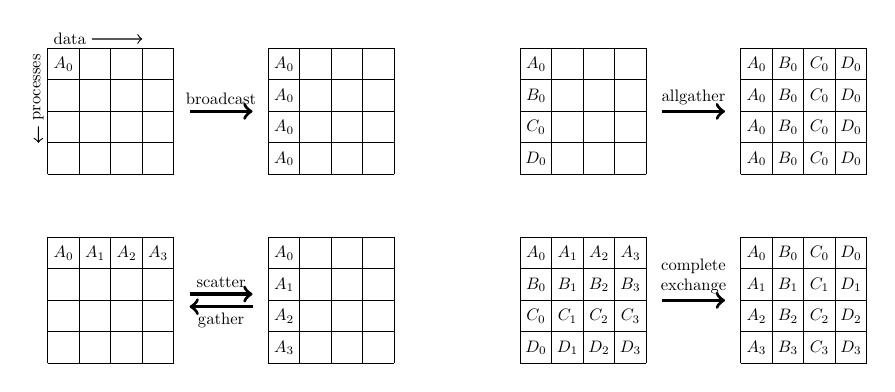
\begin{tikzpicture}[scale = 0.4, every node/.style={scale=0.6}]

\begin{scope}
	\begin{scope}
	\node[anchor = west] (Data) at (0, 4.3) {data};
	\node[anchor = east, rotate = 90] (Proc) at (-0.3, 4) {processes};
	\draw[->] (Data) -- (3, 4.3);
	\draw[->] (Proc) -- (-0.3, 1);
	\draw[step = 1cm] (0,0) grid (4,4);

	\node at (0.5, 3.5) {$A_0$};
	\end{scope}

	\draw[->, very thick] (4.5, 2) -- node[midway, above] {broadcast} (6.5, 2);

	\begin{scope}[xshift = 7cm]
	\draw[step = 1cm] (0,0) grid (4,4);

	\foreach \y in {0.5, 1.5, ..., 3.5}
		\node at (0.5, 4 - \y) {$A_0$};
	\end{scope}

	\begin{scope}[yshift = -6cm]
	\draw[step = 1cm] (0,0) grid (4,4);

	\foreach \x [count = \i from 0] in {0.5, 1.5, ..., 3.5}
		\node at (\x, 3.5) {$A_\i$};
	\end{scope}

	\draw[->, very thick] (4.5, -3.8) -- node[midway, above] {scatter} (6.5, -3.8);
	\draw[<-, very thick] (4.5, -4.2) -- node[midway, below] {gather} (6.5, -4.2);

	\begin{scope}[yshift = -6cm, xshift = 7cm]
	\draw[step = 1cm] (0,0) grid (4,4);

	\foreach \x [count = \i from 0] in {0.5, 1.5, ..., 3.5}
		\node at (0.5, 4 - \x) {$A_\i$};
	\end{scope}
\end{scope}

\begin{scope}[xshift = 15cm]
	\begin{scope}[yshift = 0cm]
	\draw[step = 1cm] (0,0) grid (4,4);

	\foreach \y/\l in {0.5/A, 1.5/B, 2.5/C, 3.5/D}
		\node at (0.5, 4 - \y) {$\l_0$};
	\end{scope}

	\draw[->, very thick] (4.5, 2) -- node[midway, above] {allgather} (6.5, 2);

	\begin{scope}[yshift = 0cm, xshift = 7cm]
	\draw[step = 1cm] (0,0) grid (4,4);

	\foreach \y in {0.5, 1.5, ..., 3.5} {
		\foreach \x/\l in {0.5/A, 1.5/B, 2.5/C, 3.5/D} {
			\node at (\x, 4 - \y) {$\l_0$};
		}
	}
	\end{scope}

	\begin{scope}[yshift = -6cm]
	\draw[step = 1cm] (0,0) grid (4,4);

	\foreach \y/\l in {0.5/A, 1.5/B, 2.5/C, 3.5/D} {
		\foreach \x[count = \i from 0] in {0.5, 1.5, ..., 3.5} {
			\node at (\x, 4 - \y) {$\l_\i$};
		}
	}
	\end{scope}

	\draw[->, very thick] (4.5, -4) -- node[midway, above, align = center] {complete \\ exchange} (6.5, -4);

	\begin{scope}[yshift = -6cm, xshift = 7cm]
	\draw[step = 1cm] (0,0) grid (4,4);

	\foreach \x/\l in {0.5/A, 1.5/B, 2.5/C, 3.5/D} {
		\foreach \y[count = \i from 0] in {0.5, 1.5, ..., 3.5} {
			\node at (\x, 4 - \y) {$\l_\i$};
		}
	}
	\end{scope}
\end{scope}

\end{tikzpicture}

\end{center}

\end{frame}



\begin{frame}[containsverbatim]
\frametitle{Collective communications}

\begin{itemize}
	\item{\verb+MPI_Bcast+ : Sends the same data to every process}
	\item{\verb+MPI_Scatter+ : Sends pieces of a buffer to every process of the communicator}
	\item{\verb+MPI_Gather+ : Retrieves pieces of data from every process}
	\item{\verb+MPI_Allgather+ : All pieces retrieved by all processes}
	\item{\verb+MPI_Reduce+ : Performs a reduction operation (\verb+MPI_SUM+, ...) across all nodes. E.g. dot product on distributed vectors}
	\item{\verb+MPI_Allreduce+ : Result distributed to all processes }
	\item{\verb+MPI_Alltoall+ : Sends all data to all processes}
	\item{{\bf Every process of the communicator must participate}. Parameters must match. Mismatches cause race conditions or deadlocks}
\end{itemize}

\end{frame}


\begin{frame}[containsverbatim]
\frametitle{Receiving image parts in order}
\begin{lstlisting}[language=C,frame=lines]
/* Generate image parts */
...
/* Each process sends */
   MPI_Isend(imgPart, partSize, MPI_BYTE, 0, 0, MPI_COMM_WORLD, &request);

// Process 0 receives all parts into buf
if (rank == 0){
   char *buf = malloc(nProcs*partSize);
   for (int i=0; i<nProcs; i++){
      MPI_Recv(buf + i*partSize, partSize, MPI_BYTE, i, 0, MPI_COMM_WORLD, MPI_STATUS_IGNORE);
   }

MPI_Wait(&request, MPI_STATUS_IGNORE);
\end{lstlisting}
\end{frame}


\begin{frame}[containsverbatim]
\frametitle{Receiving image parts out-of-order}
\begin{lstlisting}[language=C,frame=lines]
/* Generate image parts */
...
/* Each process sends */
   MPI_Isend(imgPart, partSize, MPI_BYTE, 0, 0, MPI_COMM_WORLD, &request);
// Process 0 receives all parts into buf
if (rank == 0) {
   char *buf = malloc(nProcs*partSize);
   MPI_Status s; int count;
   for (int i=0; i<nProcs; i++) {
      MPI_Probe(MPI_ANY_SOURCE, MPI_ANY_TAG, comm, &s);
      MPI_Get_count(&s, MPI_BYTE, &count);
      MPI_Recv(buf + s.MPI_SOURCE*count, count, MPI_BYTE, s.MPI_SOURCE, s.MPI_TAG, MPI_COMM_WORLD, MPI_STATUS_IGNORE);
} } MPI_Wait(&request, MPI_STATUS_IGNORE);
\end{lstlisting}
\end{frame}

\begin{frame}[containsverbatim]
\frametitle{Receiving image parts with a collective}
\begin{lstlisting}[language=C,frame=lines]
/* Generate image parts */
...
/* Process 0 is the root of the collective, i.e. the receiver of all parts */
int root = 0;
char *buf = NULL;
if (rank == root) /* Only the root must allocate buf */
   buf = malloc(nProcs*partSize)

   MPI_Gather(part, partSize, MPI_BYTE, buf, partSize, MPI_BYTE,  root, MPI_COMM_WORLD);
\end{lstlisting}
\end{frame}




\begin{frame}[containsverbatim]
\frametitle{Collectives within conditions}

Avoid collective calls within conditional clauses. What happens if :

\begin{lstlisting}[language=C,frame=lines]
int root = 0;
char *buf = NULL;
if (rank == root) { /* Only the root must allocate buf */
   buf = malloc(nProcs*partSize)

   MPI_Gather(part, partSize, MPI_BYTE, buf, partSize, MPI_BYTE,  root, MPI_COMM_WORLD);
}else{
   MPI_Send(part, ... , ... , rank, MPI_TAG);
}
\end{lstlisting}
\end{frame}


\subsection{Customization}


\begin{frame}[containsverbatim]
\frametitle{Customized communicators and datatypes}

\begin{itemize}
	\item{ You can define your own communicators : 
	\begin{itemize}
		\item{\verb+MPI_Comm_dup+ duplicates a communicator (e.g. to enable private communications within library functions)}
		\item{\verb+MPI_Comm_split+ splits a communicator into multiple smaller communicators (useful when using 2D and 3D domain decompositions) }
	\end{itemize}
	}
	\item{ You can define custom datatypes :
	\begin{itemize}
		\item{Simple structs (\verb+MPI_Type_struct+)}
		\item{Vectors (\verb+MPI_Type_vector+)}
		\item{{\bf NO POINTERS}}
	\end{itemize}
	}
\end{itemize}

\end{frame}

\subsection{Summary}

\begin{frame}[containsverbatim]
\frametitle{Does this program terminate? (assume 2 processes)}
\begin{lstlisting}[language=C,frame=lines]
int rank;
MPI_Init(&argc, &argv);
MPI_Comm_rank(&rank, MPI_COMM_WORLD);
if (rank)
  MPI_Send(&rank, 1, MPI_INT, 0, 0, MPI_COMM_WORLD);
else
  MPI_Recv(&rank, 1, MPI_INT, 1, 0, MPI_COMM_WORLD, MPI_STATUS_IGNORE);

if (rank)
  MPI_Send(&rank, 1, MPI_INT, 0, 0, MPI_COMM_WORLD);
else
  MPI_Recv(&rank, 1, MPI_INT, 1, 0, MPI_COMM_WORLD, MPI_STATUS_IGNORE);

MPI_Finalize();
\end{lstlisting}
\end{frame}

\begin{frame}[containsverbatim]
\frametitle{Timing MPI programs}

\begin{itemize}
	\item {\verb+MPI_Wtime()+ : returns a double precision floating point number, the time in seconds since some abritrary point of time in the past }
	\item {\verb+MPI_Wtick()+ : returns a double precision floating point number, the time in seconds between successive ticks of the clock }
	\item { both functions are not synchronized across the running processors. }
\end{itemize}
\end{frame}


\begin{frame}[containsverbatim]
\frametitle{Next time}

That's all for MPI 1.0. What's new in MPI2 :

\begin{itemize}
	\item {Parallel I/O}
	\item {One-sided communications}
	\item {Dynamic process management}
\end{itemize}

\end{frame}


\begin{frame}
\frametitle{Implementation of MPI}	
You don't need to have always access to a cluster or a supercomputer to develop parallel applications. Here follows some implementations of MPI :
	\begin{itemize}
	\item {\textbf{Linux} OpenMPI, MPICH2, IntelMPI (licensed)}
	\item {\textbf{MacOS X} OpenMPI (without Fortran for the official port, with if installing by hand), MPICH2 (via homebrew)}
	\item {\textbf{Windows} OpenMPI, MPICH1 (older version), MS-MPI }
	\end{itemize}
\end{frame}



%%% Local Variables: 
%%% mode: latex
%%% TeX-master: "../cours_vince"
%%% End: 


%\section{MPI advanced}
%\subsection{Introduction}

\begin{frame}[containsverbatim]
	\frametitle{What will we learn today ?}	
	\begin{itemize}
		\item {Advanced \verb+MPI_Types+, MPI communicators and groups (MPI 1.0)}
		\item {Persistent communications (MPI 2.0)}
		\item {One-sided communications (RMA) (MPI 2.0 and MPI 3.0)}
		\item {Dynamic process management (MPI 2.0)}
		\item {Parallel I/O (MPI 2.0)}
		\item {Non-blocking collectives (MPI 3.0)}
	\end{itemize}
\end{frame}


\subsection{Advanced MPI$\_$Types}


\begin{frame}[containsverbatim]
\frametitle{Basic MPI datatypes (C)}

\begin{center}
\begin{tabular}{ | l | l | }
	\hline 
	\textbf{C datatype} & \textbf{MPI datatype} \\
	\hline 
	\hline 
	signed char & MPI$\_$CHAR\\
	signed short int & MPI$\_$SHORT\\
	signed int & MPI$\_$INT \\
	signed long int & MPI$\_$LONG \\
	unsigned char & MPI$\_$UNSIGNED$\_$CHAR\\
	unsigned short int & MPI$\_$UNSIGNED$\_$SHORT\\
	unsigned long int & MPI$\_$UNSIGNED$\_$LONG\\
	unsigned int & MPI$\_$UNSIGNED\\
	float & MPI$\_$FLOAT\\
	double & MPI$\_$DOUBLE\\
	long double & MPI$\_$LONG$\_$DOUBLE\\
	\hline 
 \end{tabular}
\end{center}
\end{frame}


\begin{frame}[containsverbatim]
\frametitle{Basic MPI datatypes (FORTRAN)}

\begin{center}
\begin{tabular}{ | l | l | }
	\hline 
	\textbf{FORTRAN datatype} & \textbf{MPI datatype} \\
	\hline 
	\hline 
	INTEGER & MPI$\_$INTEGER\\
	REAL & MPI$\_$REAL\\
	REAL*8 & MPI$\_$REAL8\\
	DOUBLE PRECISION & MPI$\_$DOUBLE$\_$PRECISION\\
	COMPLEX & MPI$\_$COMPLEX\\
	LOGICAL & MPI$\_$LOGICAL\\
	CHARACTER & MPI$\_$CHARACTER \\
	\hline 
 \end{tabular}
\end{center}
\end{frame}

\begin{frame}[containsverbatim]
\frametitle{Derived MPI datatypes}

OK. That is perfect when all the data are of the same type (integers, floats, characters, etc..). But how to send a structure using MPI ?

\begin{lstlisting}[language=C,frame=lines]
struct { 
   int x; int y;
   double vx; double vy;
   float mass;
} particle;
particle p = {1,2,0.3,0.4,1.0};
MPI_Send(p, ...);
\end{lstlisting}
\end{frame}


\begin{frame}[containsverbatim]
\frametitle{Derived MPI datatypes}
\begin{itemize}
	\item Definition of \textbf{new} datatypes by grouping basic MPI datatypes
	\item It is possible to group \begin{itemize} \item data from different types \item group non-contiguous data \end{itemize}
	\item A derived datatype is defined in three steps : \begin{itemize} \item construct the type \item commit it to the system \item free it \end{itemize}
\end{itemize}

\end{frame}



\begin{frame}[containsverbatim]
\frametitle{Derived MPI datatypes}	
\begin{itemize}
	\item \verb+MPI_Type_contiguous+ Produces a new data type by making copies of an existing data type. 
	\item \verb+MPI_Type_vector+, Similar to contiguous, but allows for regular gaps (stride) in the displacements
	\item \verb+MPI_Type_indexed+, An array of displacements of the input data type is provided as the map for the new data type.
	\item \verb+MPI_Type_create_struct+ The new data type is formed according to completely defined map of the component data types. 
	\item \verb+MPI_Type_extent+ Returns the size in bytes of the specified data type.
	\item \verb+MPI_Type_commit+ Commits new datatype to the system. 
	\item \verb+MPI_Type_free+ Deallocates the specified datatype object.
\end{itemize}

\end{frame}

\begin{frame}[containsverbatim]
\frametitle{MPI$\_$Type$\_$struct example}	

\begin{lstlisting}[language=C,frame=lines,basicstyle=\footnotesize]
struct foo { int a; char b; } f ; f.a = 1; f.b = 'z';
int blen[2];
MPI_Aint displs[2];
MPI_Datatype oldtypes[2];
MPI_Datatype newtype;

MPI_Aint zero_address, first_address, second_address;
MPI_Get_address(&f, &zero_address);
MPI_Get_address(&f.a, &first_address);
MPI_Get_address(&f.b, &second_address);
blen[0] = 1; displs[0] = MPI_Aint_diff(first_address, zero_address);
oldtypes[0] = MPI_INT; oldtypes[1] = MPI_CHAR;
blen[1] = 1; displs[1] = MPI_Aint_diff(second_address, zero_address);
MPI_Type_create_struct( 2, blen, displs, oldtypes, &newtype );
MPI_Type_commit(&newtype);

MPI_Send(&f, 1, newtype, 0, 100, MPI_COMM_WORLD );
MPI_Type_free( &newtype );
\end{lstlisting}
The MPI datatype \texttt{newtype} is a structure that contains \texttt{\{f\}}



%\begin{frame}[containsverbatim]
%\frametitle{MPI$\_$Type$\_$struct example}	

%\begin{lstlisting}[language=C,frame=lines]
%struct { int a; char b; } foo;
%foo f = {1,'z'};
%MPI_Aint zero_address, first_address, second_address;
%MPI_Get_address(&foo, &zero_address);
%MPI_Get_address(&foo.a, &first_address);
%MPI_Get_address(&foo.b, &second_address);
%MPI_Datatype newtype;
%MPI_Aint displs[2];
%blen[0] = 1; indices[0] = MPI_Aint_diff(first_address, zero_address);
%oldtypes[0] = MPI_INT; oldtypes[1] = MPI_CHAR;
%blen[1] = 1; indices[1] = MPI_Aint_diff(second_address, zero_address); 
%MPI_Type_create_struct( 2, blen, indices, oldtypes, &newtype );
%MPI_Type_Commit(&newtype);
%MPI_Send(&f, 1, newtype, 0, 100, MPI_COMM_WORLD );
%MPI_Type_free( &newtype );
%\end{lstlisting}
%The MPI datatype \texttt{newtype} is a structure that contains \texttt{\{foo\}}



% =============================================================
% EXOS 2018 avec correction
% =============================================================
%  MPI_Aint zero_address, first_address, second_address;                            
%  MPI_Get_address(&send, &zero_address);                                            
%  MPI_Get_address(&send.sum, &first_address);                                      
%  MPI_Get_address(&send.rank, &second_address);                                    
%                                                                                    
%  MPI_Aint displs[2];                                                              
%  displs[0] = MPI_Aint_diff(first_address, zero_address);;                          
%  displs[1] = MPI_Aint_diff(second_address, zero_address);                        
%                                                                                    
%  MPI_Datatype types[2] = {MPI_DOUBLE, MPI_INT};                                    
%  MPI_Datatype sum_t;                                                              
%  MPI_Type_create_struct(2, blk_length, displs, types, &sum_t);                    
%  MPI_Type_commit(&sum_t)
% =============================================================


%\begin{lstlisting}[language=C,frame=lines]
%int blocklens[7];
%MPI_Datatype myparticle;
%MPI_Datatype old_types[5];
%old_types[0] = MPI_INT; old_types[1] = MPI_INT;
%old_types[2] = MPI_DOUBLE; old_types[3] = MPI_DOUBLE;
%old_types[4] = MPI_FLOAT;
%blocklens[0] = 1; blocklens[1] = 1; blocklens[2] = 1;
%blocklens[3] = 1; blocklens[4] = 1;
%MPI_Address( &particle.x, &indices[0] ); MPI_Address( &particle.y, &indices[1] );
%MPI_Address( &particle.vx, &indices[2] ); MPI_Address( &particle.vy, &indices[3] );
%MPI_Address( &particle.mass, &indices[4] );
%MPI_Type_struct( 5, blocklens, indices, old_types, &myparticle );
%MPI_Send( &p, 1, myparticle, 0, 100, MPI_COMM_WORLD );
%MPI_Type_free( &myparticle );
%\end{lstlisting}

\end{frame}

\begin{frame}[containsverbatim]
\frametitle{Extents}	
FIXME : MPI_Type_create_resized()
\end{frame}





\begin{frame}[containsverbatim]
\frametitle{Pack/Unpack data}	
\begin{itemize}
	\item { Instead of creating a new datatype, it is possible to pack and unpack data of different types }
	\item { Less good than MPI derived datatypes in terms of memory usage and performance }
	\item { ``just like a streaming'' }
	\item { \verb+int MPI_Pack(const void *inbuf, int incount, +\\\verb+MPI_Datatype datatype, void *outbuf, int outsize,+\\\verb+ int *position, MPI_Comm comm)+}
	\item { \verb+int MPI_Unpack(const void *inbuf, int insize,+\\\verb+ int *position, void *outbuf, int outcount, +\\\verb+MPI_Datatype datatype, MPI_Comm comm)+}
\end{itemize}
\end{frame}


\begin{frame}[containsverbatim]
\frametitle{Pack/Unpack data}	
\begin{lstlisting}[language=C,frame=lines]
int x; float a, int position=0;
char buffer[100];
if (myrank==0)
   MPI_Pack(&a, 1, MPI_FLOAT, buffer, 100, &position, MPI_COMM_WORLD)
   MPI_Pack(&x, 1, MPI_INT, buffer, 100, &position, MPI_COMM_WORLD)
   MPI_Send(buffer, 100, MPI_PACKED, 1, 999, MPI_COMM_WORLD);
}else if (myrank==1) {
   MPI_Recv(buffer, 100, MPI_PACKED, 0, 999, MPI_COMM_WORLD, status)
   MPI_Unpack(buffer, 100, &position, &a, 1, MPI_FLOAT, MPI_COMM_WORLD);
   MPI_Unpack(buffer, 100, &position, &x, 1, MPI_INT, MPI_COMM_WORLD);
}
\end{lstlisting}
\end{frame}


\subsection{MPI communicators and groups}



\begin{frame}[containsverbatim]
\frametitle{MPI Groups and Communicators}	
MPI Groups :
\begin{itemize}
	\item {ordered set of processes}
	\item {each process has an unique ID (rank within the group) and can belong to several different groups}
	\item {a group can be used to create a new communicator}
\end{itemize}
MPI Communicators :
\begin{itemize}
	\item {A group of processes}
	\item {encapsulate the communications between the belonging processes}
	\item {An MPI communication can take place only with a communicator (not a group)}
\end{itemize}
\end{frame}


\begin{frame}[containsverbatim]
\frametitle{MPI Groups and Communicators}	
\begin{center}
% Slide 194
\begin{tikzpicture}[scale=0.7, every node/.style={scale=0.8}]
\node[label = {above:\texttt{MPI\_COMM\_WORLD}}, ellipse, draw, minimum height = 3cm, minimum width = 6cm, dashed, outer sep = 3pt] (W) at (0,0) {};

\node[circle, draw, inner sep = 3pt] at (-2, 0) {2};
\node[circle, draw, inner sep = 3pt] at (-1.3, -0.3) {1};
\node[circle, draw, inner sep = 3pt] at (-1, 0.4) {6};
\node[circle, draw, inner sep = 3pt] at (-0.2, 0) {0};
\node[circle, draw, inner sep = 3pt] at (0.4, 0.5) {7};
\node[circle, draw, inner sep = 3pt] at (0.6, -0.5) {3};
\node[circle, draw, inner sep = 3pt] at (1.3, 0) {5};
\node[circle, draw, inner sep = 3pt] at (2.3, 0) {4};

\node[ellipse, label = {left:{Group 1}}, minimum height = 2cm, minimum width = 3cm] (G1) at (-3, -3) {};
\node[circle, draw, inner sep = 3pt] at (-3.4, -2.6) {1};
\node[circle, draw, inner sep = 3pt] at (-2.6, -2.6) {3};
\node[circle, draw, inner sep = 3pt] at (-3.8, -3.3) {2};
\node[circle, draw, inner sep = 3pt] at (-3, -3.3) {0};
\node[circle, draw, inner sep = 3pt] at (-2.2, -3.3) {4};

\node[ellipse, label = {right:{Group 2}}, minimum height = 2cm, minimum width = 1.5cm] (G2) at (3, -3) {};
\node[circle, draw, inner sep = 3pt] at (3.2, -3.4) {7};
\node[circle, draw, inner sep = 3pt] at (3.2, -2.6) {6};
\node[circle, draw, inner sep = 3pt] at (2.5, -3) {5};

\draw[->] (W) -- (G1);
\draw[->] (W) -- (G2);

\begin{scope}[yshift = -2.6cm]
\node[draw, blue2, outer sep = 3pt, dashed, ellipse, label = {below:{MPI Communicator (Group1)}}, minimum height = 2cm, minimum width = 3cm] (GC1) at (-3, -3) {};
\node[circle, draw, inner sep = 3pt] at (-3.4, -2.6) {1};
\node[circle, draw, inner sep = 3pt] at (-2.6, -2.6) {3};
\node[circle, draw, inner sep = 3pt] at (-3.8, -3.3) {2};
\node[circle, draw, inner sep = 3pt] at (-3, -3.3) {0};
\node[circle, draw, inner sep = 3pt] at (-2.2, -3.3) {4};

\node[draw, blue2, outer sep = 3pt, dashed, ellipse, label = {below:{MPI Communicator (Group2)}}, minimum height = 2cm, minimum width = 3cm] (GC2) at (3, -3) {};
\node[circle, draw, inner sep = 3pt] at (3.2, -3.4) {7};
\node[circle, draw, inner sep = 3pt] at (3.2, -2.6) {6};
\node[circle, draw, inner sep = 3pt] at (2.5, -3) {5};
\end{scope}

\draw[->] (G1) -- (GC1);
\draw[->] (G2) -- (GC2);

\end{tikzpicture}

\end{center}
\end{frame}



\begin{frame}[containsverbatim]
\frametitle{Create a new communicator}	

%\begin{lstlisting}[language=C,frame=lines]
%main(int argc, char *argv[])  {
% int myrank, new_rank, sendbuf, recvbuf, mysize,
% MPI_Group  old_grp, new_grp;
% MPI_Comm   new_comm;
% MPI_Init(&argc,&argv);
% MPI_Comm_rank(MPI_COMM_WORLD, &rank);
% MPI_Comm_size(MPI_COMM_WORLD, &size);
% MPI_Comm_group(MPI_COMM_WORLD, &old_group);
% if (rank < NPROCS/2) {
%  MPI_Group_incl(old_grp, size/2, ranks1, &new_grp);
% } else {
%  MPI_Group_incl(old_grp, size/2, ranks2, &new_grp);
% }
% MPI_Comm_create(MPI_COMM_WORLD,new_group,&new_comm);
% MPI_Group_rank (new_group, &new_rank);
% printf("rank= %d newrank= %d recvbuf= %d\n",rank,new_rank,recvbuf);
% MPI_Finalize();
%}
%\end{lstlisting}


\begin{lstlisting}[language=C,frame=lines]
 MPI_Init(&argc,&argv);
 MPI_Comm_rank(MPI_COMM_WORLD, &rank);
 MPI_Comm_size(MPI_COMM_WORLD, &size);
 MPI_Comm_group(MPI_COMM_WORLD, &old_g);
 int nbr_g1 = 5;
 ranks1 = (int*) malloc(nbr_g1*sizeof(int));
 ranks2 = (int*) malloc((size-nbr_g1)*sizeof(int));
 for (i=0;i<nbr_grp1;i++)  ranks1[i]=i;
 for (i=0;i<(size-nbr_g1);i++) ranks2[i]=size-i-1;
 if (rank < nbr_g1) {
  MPI_Group_incl(old_g,nbr_g1,ranks1,&new_g);
 } else {
  MPI_Group_incl(old_g,(size-nbr_g1),ranks2,&new_g);
 } 
 MPI_Comm_create(MPI_COMM_WORLD,new_g,&new_comm);
 MPI_Group_rank (new_g, &new_rank);
 printf("rank %d grprank is %d \n",rank,new_rank);
 MPI_Finalize();
\end{lstlisting}


%\begin{lstlisting}[language=C,frame=lines]
% MPI_Group  old_grp, new_grp;
% MPI_Comm   new_comm;
% MPI_Init(&argc,&argv);
% MPI_Comm_rank(MPI_COMM_WORLD, &rank);
% MPI_Comm_size(MPI_COMM_WORLD, &size);
% MPI_Comm_group(MPI_COMM_WORLD, &old_group);
% if (rank < NPROCS/2) {
%  MPI_Group_incl(old_grp, size/2, ranks1, &new_grp);
% } else {
%  MPI_Group_incl(old_grp, size/2, ranks2, &new_grp);
% }
% MPI_Comm_create(MPI_COMM_WORLD,new_group,&new_comm);
% MPI_Group_rank (new_group, &new_rank);
% printf("rank= %d newrank= %d recvbuf= %d\n",rank,new_rank,recvbuf);
% MPI_Finalize();
%\end{lstlisting}


\end{frame}


\subsection{Persistent communications}

\begin{frame}[containsverbatim]
\frametitle{Persistent communications}
\begin{itemize}
	\item {when a same communication is repeated within a loop (e.g. exchanging neighbors in 2D Poisson) }
	\item {Improvement can be done using a persistent communication}
	\item {Using a \verb+MPI_Request+ to initiate and complete a communication}
	\item {\verb+MPI_Send_Init()+ : creates a persistent communication request for a standard mode send operation }
	\item {\verb+MPI_Bsend_Init()+ : creates a persistent communication request for a bufferd mode send operation}
	\item {\verb+MPI_Ssend_Init()+ : creates a persistent communication object for a synchronous mode send operation}
	\item {\verb+MPI_Rsend_Init()+ : creates a persistent communication object for a ready mode send operation}
	\item {\verb+MPI_Recv_Init()+ : creates a persistent communication request for a receive operation.}
\end{itemize}
\end{frame}


\begin{frame}[containsverbatim]
\frametitle{Persistent communications example}	

\begin{lstlisting}[language=C,frame=lines,basicstyle=\footnotesize]
   MPI_Request recvreq;
   MPI_Request sendreq;

   MPI_Recv_init (buffer, N, MPI_FLOAT, rank-1, tag_check_infos, MPI_COMM_WORLD, &recvreq);
   MPI_Send_init (buffer, N, MPI_FLOAT, rank+1, tag_check_infos, MPI_COMM_WORLD, &sendreq);

/* ... copy stuff into buffer ... */

   MPI_Start(&sendreq);         
   MPI_Start(&recvreq);         
   MPI_Wait(&sendreq, &status); 
   MPI_Wait(&recvreq, &status); 

   MPI_Request_free( &recvreq );
   MPI_Request_free( &sendreq );
\end{lstlisting}
\end{frame}




\subsection{Remote Memory Access (One-sided communications)}

\begin{frame}[containsverbatim]
\frametitle{One-sided communication}
\begin{itemize}
	\item {A MPI process can access another MPI process's memory space directly (RMA)}
	\item {No explicit coordination between both processes}
	\item {explicit transfer, explicit synchronization}
	\item {Better performance}
\end{itemize}
\end{frame}

\begin{frame}[containsverbatim]
\frametitle{One-sided communication}
Initialization/Free (of the \textit{window} = window in memory)
\begin{itemize}
	\item {\verb+MPI_Alloc_Mem()+, \verb+MPI_Free_Mem()+}
	\item {\verb+MPI_Win_Create()+, \verb+MPI_Win_Free()+}
\end{itemize}
Remote memory access
\begin{itemize}
	\item {\verb+MPI_Put()+ (like send)}
	\item {\verb+MPI_Get()+ (like recv)}
	\item {\verb+MPI_Accumulate()+ (like reduce)}
\end{itemize}
Synchronization
\begin{itemize}
	\item {\verb+MPI_Win_Fence()+}
	\item {\verb+MPI_Win_Post()+, \verb+MPI_Win_Start()+, \verb+MPI_Win_Complete()+, \verb+MPI_Win_Wait()+}
	\item {\verb+MPI_Win_Lock()+, \verb+MPI_Win_Unlock()+}
\end{itemize}

\end{frame}

\begin{frame}[containsverbatim]
\frametitle{Memory allocation}
\begin{itemize}
	\item {allocate \verb+size+ of memory segments in bytes}
	\item {\verb+info+ can be used to provide directives that control the desired location of the allocated memory}
	\item {\verb+*baseptr+ is the pointer to the beginning of the memory segment}
\end{itemize}

\begin{lstlisting}[language=C,frame=lines]
int MPI_Alloc_mem(MPI_Aint size, MPI_Info info, void *baseptr)
\end{lstlisting}

\end{frame}



\begin{frame}[containsverbatim]
\frametitle{Memory \texttt{window} creation}
\begin{itemize}
	\item {A \verb+MPI_Win+ is an opaque object which can be reused to perform one-sided communication}
	\item {A \verb+window+ is a specified region in memory that can be accessed by another process}
\end{itemize}

\begin{lstlisting}[language=C,frame=lines]
int MPI_Win_create(void *base, MPI_Aint size, int disp_unit, MPI_Info info, MPI_Comm comm, MPI_Win *win)
\end{lstlisting}

where \verb+base+ is the initial address of the region, of \verb+size+ length of size \verb+disp_unit+ in bytes.

\end{frame}

\begin{frame}[containsverbatim]
\frametitle{\texttt{Put}/\texttt{Get} within the \texttt{window}}
\begin{itemize}
	\item {close to an \verb+MPI_Send+ call with 
		\begin{itemize}
			\item {\textit{what to send} : \verb+origin_addr+ start of the buffer of size \verb+origin_count+ of type \verb+origin_datatype+}
			\item {\textit{to which process} : \verb+target_rank+ at the place \verb+target_count+ of type \verb+target_datatype+}
			\item {\textit{in which context} : within the window \verb+win+}
		\end{itemize}
	}
%	\item {}
\end{itemize}

\begin{lstlisting}[language=C,frame=lines]
int MPI_Put(const void *origin_addr, int origin_count, MPI_Datatype origin_datatype, int target_rank, MPI_Aint target_disp, int target_count, MPI_Datatype target_datatype, MPI_Win win)
\end{lstlisting}

\begin{lstlisting}[language=C,frame=lines]
int MPI_Get(void *origin_addr, int origin_count, MPI_Datatype origin_datatype, int target_rank, MPI_Aint target_disp, int target_count, MPI_Datatype target_datatype, MPI_Win win)
\end{lstlisting}


\end{frame}


\begin{frame}[containsverbatim]
\frametitle{One-sided communications example}

\begin{lstlisting}[language=C,frame=lines]
MPI_Win win;
int *mem;
float x = 1.0;
MPI_Alloc_mem(size * sizeof(int), MPI_INFO_NULL, &mem);
MPI_Win_create(mem, size * sizeof(int), sizeof(int), MPI_INFO_NULL, MPI_COMM_WORLD, &win);

// Write x at position 0 within process ranks's memory
MPI_Put(&x, 1, MPI_FLOAT, 0, rank, 1, MPI_INT, win);

MPI_Win_free(win);
MPI_Free_mem(mem);
\end{lstlisting}


\end{frame}


\begin{frame}[containsverbatim]
\frametitle{One-sided communications remarks}

\begin{itemize}
%	\item {Three primitives : Put (like a send), Get (like a recv) and accumulate (like a reduction)}
%	\item {synchronizations : fence / post-start-complete-wait / lock-unlock}
	\item {Pay attention to the memory coherence}
	\item {Can be dangerous : how a process knows if its data are in use/modified ?}
	\item {MPI-3 provides new features : \begin{itemize}
			\item cache-coherent windows,
			\item new primitives \verb+MPI_Get_accumulate()+, \verb+MPI_Fetch_and_op()+, \verb+MPI_Compare_and_swap+,
			\item requested-based primitives like \verb+MPI_R{put,get,accumulate,get_accumulate}+,
			\item ``all''-versions of the synchronization routines : \verb+MPI_Win_{un}lock_all+, \verb+MPI_Win_flush{_all}+, \verb+MPI_Win_flush_local{_all}+
			\end{itemize}
	}
%	\item {}
\end{itemize}
\end{frame}



\subsection{Dynamic Process Management}


\begin{frame}[containsverbatim]
\frametitle{Static model vs. Dynamic model}
MPI 1:
\begin{itemize}
	\item {Fixed number of MPI processes}
	\item {What happens if a process fail ? The entire job fails.}
	\item {impossible to ``inter-connect'' two independent MPI running jobs}
\end{itemize}
MPI 2 / MPI 3:
\begin{itemize}
	\item {support the creation of processes \textbf{on the fly} that can connect to existing running processes}
%	\item {\verb+MPI_Comm_spawn+ objects}
	\item {Concept of \textbf{intercommunicator} to handle the communications between parents and children}
	\item {Tricky !!}
\end{itemize}
\end{frame}


\begin{frame}[containsverbatim]
\frametitle{Master-Slave example (www.mpi-forum.org) -- Master}
\begin{lstlisting}[language=C,frame=lines]
int main(int argc, char *argv[]) { 
   int world_size, universe_size, *universe_sizep, flag; 
   MPI_Comm everyone;           /* intercommunicator */ 
   char worker_program[100]; 
   MPI_Init(&argc, &argv); 
   MPI_Comm_size(MPI_COMM_WORLD, &world_size); 
   MPI_Attr_get(MPI_COMM_WORLD, MPI_UNIVERSE_SIZE, &universe_sizep, &flag);  
   universe_size = *universe_sizep; 
   choose_worker_program(worker_program); 
   MPI_Comm_spawn(worker_program, MPI_ARGV_NULL, universe_size-1, MPI_INFO_NULL, 0, MPI_COMM_SELF, &everyone, MPI_ERRCODES_IGNORE); 
/ * Parallel code here.  */
   MPI_Finalize(); 
   return 0; }
\end{lstlisting}
\end{frame}


\begin{frame}[containsverbatim]
\frametitle{Master-Slave example (www.mpi-forum.org) -- Slave}
\begin{lstlisting}[language=C,frame=lines]
int main(int argc, char *argv[]) { 
   int size; 
   MPI_Comm parent; 
   MPI_Init(&argc, &argv); 
   MPI_Comm_get_parent(&parent); 
   if (parent == MPI_COMM_NULL) error("No parent!"); 
   MPI_Comm_remote_size(parent, &size); 
   if (size != 1) error("Something's wrong with the parent"); 
 
/ * Parallel code here.  */

   MPI_Finalize(); 
   return 0; 
} 
\end{lstlisting}
\end{frame}



\subsection{Parallel I/O with MPI}

\begin{frame}[containsverbatim]
\frametitle{Introducing remarks}
\begin{itemize}
	\item {I/O is often (if not always) the main bottleneck in a parallel application}
	\item {MPI provides a mechanism to read/write in parallel}
\end{itemize}

\begin{center}
% Slide 208
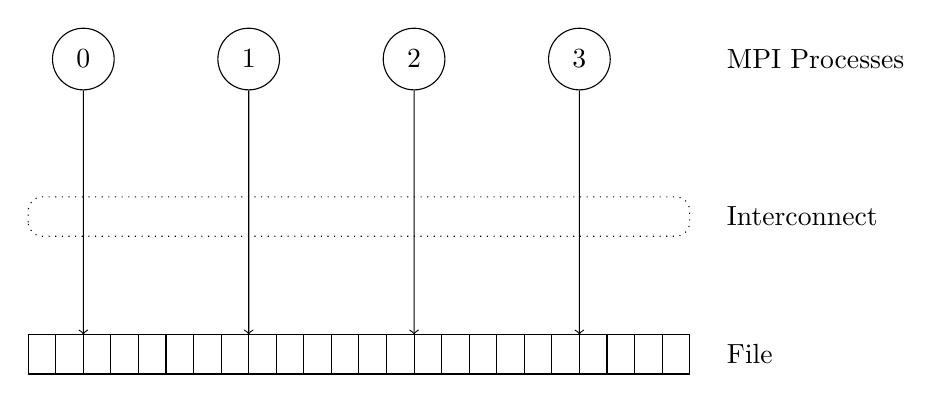
\begin{tikzpicture}[xscale = 0.7]

\draw[step = 0.5cm] (0,0) grid (12, 0.5);

\foreach \x[count = \i from 0] in {1, 4, ..., 10} {
	\node[circle, draw, inner sep = 5pt] (\i) at (\x, 4) {\i};
	\draw[->] (\i) -- (\x, 0.5);
}

\node[anchor = west] at (12.5, 4) {MPI Processes};
\node[anchor = west] at (12.5, 2) {Interconnect};
\node[anchor = west] at (12.5, 0.25) {File};

\draw[dotted, rounded corners = 5pt] (0,1.75) rectangle (12, 2.25);


\end{tikzpicture}

\end{center}
\end{frame}


\begin{frame}[containsverbatim]
\frametitle{Introducing remarks}
\begin{itemize}
	\item {MPI IO API works on your desktop/laptop}
	\item {Most of the large HPC systems have a \textbf{parallel file system} (like GPFS, Lustre, etc..)}
	\item {If the file is distributed smartly on a parallel file system : performance increases}
	\item {MPI IO offers a high-level API to access a distributed file (no needs to implement complexe POSIX calls)}
	\item {\textbf{does not work with ASCII files}}
	\item {Most of the standard file format support MPI IO (e.g. HDF5, NetCDF, etc..)}
\end{itemize}
\end{frame}


\begin{frame}[containsverbatim]
\frametitle{Poisson so far}
\begin{center}
% Slide 210
\begin{tikzpicture}[xscale = 0.8]


\foreach \x/\c[count = \i from 0] in {0/blue8, 3/blue4, 6/yellowbrown4, 9/yellowbrown2} {
	\node[outer sep = 3pt, fill = \c!40!white, circle, draw, inner sep = 5pt] (\i) at (\x, 4) {\i};
	\fill[\c!40!white] (\x, 0) rectangle (\x + 3, 0.5);
}

\draw[step = 0.5cm] (0,0) grid (12, 0.5);

\draw[->] (1) to[bend left] (0);
\draw[->] (2) to[bend left] (0);
\draw[->] (3) to[bend left] node[pos = 0.3, right, xshift = 0.5cm] {\texttt{MPI\_send(mypart, 0)}} (0);

\draw[->] (0.north east) to[out = 70, in = 110, looseness = 2] (0.north west);
\draw[->] (0) to[bend right] node[midway, right] {\texttt{Write()}} (-0.05, 0.55);
\end{tikzpicture}

\end{center}
\end{frame}

\begin{frame}[containsverbatim]
\frametitle{Poisson ideal}
\begin{center}
% Slide 210
\begin{tikzpicture}[xscale = 0.8]


\foreach \x/\c[count = \i from 0] in {0/blue8, 3/blue4, 6/yellowbrown4, 9/yellowbrown2} {
	\node[outer sep = 3pt, fill = \c!40!white, circle, draw, inner sep = 5pt] (\i) at (\x, 4) {\i};
	\fill[\c!40!white] (\x, 0) rectangle (\x + 3, 0.5);
	\draw[->] (\i) -- (\x, 0.55);
}

\node[anchor = west] at (9, 2) {\texttt{MPI\_File\_Write()}};

\draw[step = 0.5cm] (0,0) grid (12, 0.5);

\end{tikzpicture}

\end{center}
\end{frame}


\begin{frame}[containsverbatim]
\frametitle{Open/Close a file in parallel}
\begin{itemize}
	\item {\verb+comm+ : the communicator that contains the writing/reading MPI processes}
	\item {\verb+*filename+ : a file name}
	\item {\verb+amode+ : file access mode (Read only \verb+MPI_MODE_RDONLY+, read/write \verb+MPI_MODE_RDWR+, create \verb+MPI_MODE_CREATE+, etc..)}
	\item {\verb+info+ : file info object}
	\item {\verb+*fh+ : file handle}
\end{itemize}

\begin{lstlisting}[language=C,frame=lines]
int MPI_File_open(MPI_Comm comm, const char *filename, int amode, MPI_Info info, MPI_File *fh)
\end{lstlisting}

\begin{lstlisting}[language=C,frame=lines]
int MPI_File_close(MPI_File *fh)
\end{lstlisting}
\textbf{Collective calls !!}
\end{frame}


\begin{frame}[containsverbatim]
\frametitle{etype, offset and displacement}
\begin{itemize}
	\item {\textbf{etype} is the elementary type of the data of the parallel accessed file}
	\item {\textbf{offset} is a position in the file in term of multiple of etypes}
	\item {\textbf{displacement} of a position within the file is the number of bytes from the beginning of the file}
\end{itemize}
\begin{center}
% Slide 213
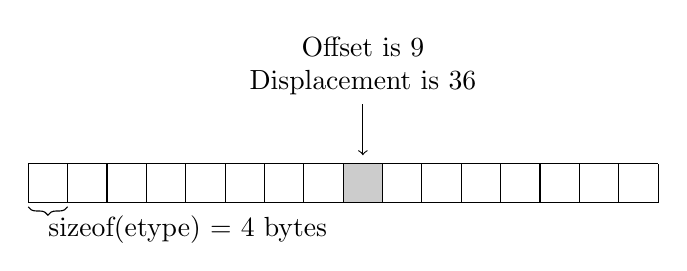
\begin{tikzpicture}
\draw[step = 0.5cm] (0,0) grid (8, 0.5);

\node[rectangle, draw, inner sep = 0.25cm, fill = gray!40!white, outer sep = 3pt] (R) at (4.25, 0.25) {};
\node[align = center, anchor = south] (W) at (4.25, 1.25) {Offset is 9 \\ Displacement is 36};

\draw[<-] (R) -- (W);

\draw[decorate,decoration={brace,amplitude=3pt, mirror}] (0, -0.05) -- (0.5, -0.05);
\node[anchor = north west, inner sep = 0pt] at (0.25, -0.15) {sizeof(etype) = 4 bytes};

\end{tikzpicture}

\end{center}
\end{frame}


\begin{frame}[containsverbatim]
\frametitle{Simple independent read/write}
\begin{itemize}
	\item {Can be used from a single (or group) of processes}
	\item {The \verb+offset+ must be specified in the \verb+*buf+ buffer}
	\item {\verb+count+ elements of type \verb+datatype+ are written}
\end{itemize}
\begin{lstlisting}[language=C,frame=lines]
int MPI_File_write_at(MPI_File fh, MPI_Offset offset, ROMIO_CONST void *buf, int count, MPI_Datatype datatype, MPI_Status *status)
\end{lstlisting}
\begin{lstlisting}[language=C,frame=lines]
int MPI_File_read_at(MPI_File fh, MPI_Offset offset, void *buf,int count, MPI_Datatype datatype, MPI_Status *status)
\end{lstlisting}
\end{frame}


\begin{frame}[containsverbatim]
\frametitle{\texttt{view} by each process}
\begin{itemize}
	\item {Initialy, each process view the file as a linear byte stream and each process views data in its own native representation}
	\item {this is changed using \verb+MPI_File_set_view+}
	\item {\verb+disp+ is the displacement (defines the beginning of the data of the file that belongs to the process) in bytes}
	\item {\verb+etype+ is the elementary type}
\end{itemize}
\begin{lstlisting}[language=C,frame=lines]
int MPI_File_set_view(MPI_File fh, MPI_Offset disp, MPI_Datatype etype, MPI_Datatype filetype, ROMIO_CONST char *datarep, MPI_Info info)
\end{lstlisting}
\begin{lstlisting}[language=C,frame=lines]
int MPI_File_get_view(MPI_File fh, MPI_Offset *disp, MPI_Datatype *etype, MPI_Datatype *filetype, char *datarep)
\end{lstlisting}
\end{frame}

\begin{frame}[containsverbatim]
\frametitle{Setting up a \texttt{view}}
\begin{center}
% Slide 216
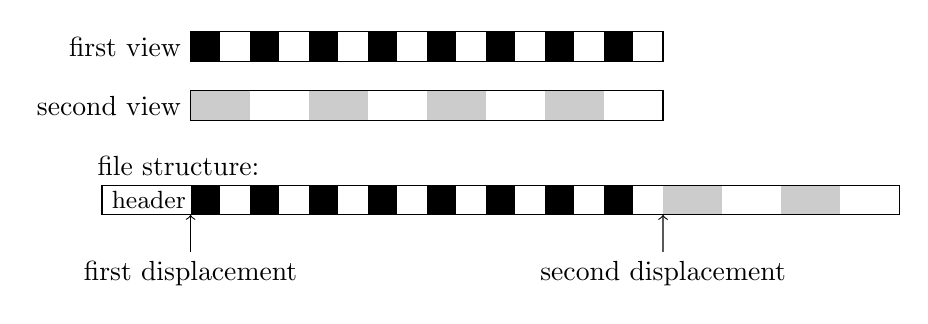
\begin{tikzpicture}[scale=0.75]

\node[anchor = east] at (0, 1.25) {first view};
\node[anchor = east] at (0, 0.25) {second view};

\foreach \x in {0, 1, 2, ..., 7.5}
	\fill[black] (\x, 1) rectangle (\x + 0.5, 1.5);

\foreach \x in {0, 2, ..., 7.5}
	\fill[gray!40!white] (\x, 0) rectangle (\x + 1, 0.5);

\draw (0, 1) rectangle (8, 1.5);
\draw (0, 0) rectangle (8, 0.5);

\begin{scope}[yshift = -1.6cm]
\node[anchor = south west, xshift = -0.18cm] at (-1.5, 0.5) {file structure:};

\node[anchor = west] at (-1.5, 0.25) {\small header};

\foreach \x in {0, 1, 2, ..., 7.5}
	\fill[black] (\x, 0) rectangle (\x + 0.5, 0.5);

\foreach \x in {0, 2, ..., 3.5}
	\fill[gray!40!white] (\x + 8, 0) rectangle (\x + 9, 0.5);

\draw (-1.5, 0) rectangle (12, 0.5);

\node (D1) at (0, -1) {first displacement};
\node (D2) at (8, -1) {second displacement};

\draw[->] (D1) -- (0,0);
\draw[->] (D2) -- (8,0);
\end{scope}

\end{tikzpicture}

\end{center}
(source : MPI 2.2 specifications)
\end{frame}

\begin{frame}[containsverbatim]
\frametitle{Simple independent read/write without offset}
\begin{itemize}
	\item {the \texttt{view} is specified prior to the call }
\end{itemize}
\begin{lstlisting}[language=C,frame=lines]
int MPI_File_write(MPI_File fh, ROMIO_CONST void *buf, int count, MPI_Datatype datatype, MPI_Status *status)
\end{lstlisting}
\begin{lstlisting}[language=C,frame=lines]
int MPI_File_read(MPI_File fh, void *buf, int count,MPI_Datatype datatype, MPI_Status *status)
\end{lstlisting}
\end{frame}


\begin{frame}[containsverbatim]
\frametitle{Collective read/write with/without offset}
\begin{itemize}
	\item {Same structure than Independent routines but with \verb+_all+ at the end }
	\item {for instance : }
\end{itemize}
\begin{lstlisting}[language=C,frame=lines]
int MPI_File_write_all(MPI_File fh, ROMIO_CONST void *buf, int count, MPI_Datatype datatype, MPI_Status *status)
\end{lstlisting}
\end{frame}


\begin{frame}[containsverbatim]
\frametitle{MPI-IO on a cartesian grid Using subarrays}
\begin{itemize}
	\item {subarray from a structured data grid}
	\item {definition of subarrays leads to a collective call}
	\item {definition of a pattern}
	\item {hallos (or ghostcells) are allowed}
	\item {like defining a new datatype}
	\item {subarrays \textbf{must} have the same size on each process}
\end{itemize}
\begin{lstlisting}[language=C,frame=lines]
int MPI_Type_create_subarray(int ndims, const int array_of_sizes[], const int array_of_subsizes[], const int array_of_starts[], int order, MPI_Datatype oldtype, MPI_Datatype *newtype)
\end{lstlisting}
\end{frame}

\subsection{Virtual topology}

\begin{frame}[containsverbatim]
\frametitle{Parenthesis : Virtual Topology}
\frametitle{Virtual Topology}
\begin{itemize}
	\item {A subarray must be mapped onto a topology}
	\item {It is done through the creation of a new communicator}
	\item {Cartesian topology fits with subarrays from a regular cartesian grid}
\end{itemize}
\begin{lstlisting}[language=C,frame=lines]
int MPI_Cart_create(MPI_Comm comm_old, int ndims, const int dims[], const int periods[], int reorder, MPI_Comm *comm_cart)
\end{lstlisting}
\end{frame}


\begin{frame}[containsverbatim]
\frametitle{Virtual topology example}
\begin{center}
\includegraphics[width=8cm]{Day3/images/topology.eps}
\end{center}
(source : Andrew Siegel, University of Chicago)
\end{frame}


\begin{frame}[containsverbatim]
\frametitle{Virtual topology example}
\begin{lstlisting}[language=C,frame=lines]
gsizes[0] = m; // no. of rows in global array
gsizes[1] = n; // no. of columns in global array
psizes[0] = 2; // no. of procs. in vert. dimension
psizes[1] = 3; // no. of procs. in hori. dimension
lsizes[0] = m/psizes[0]; // no. of rows in local array
lsizes[1] = n/psizes[1]; // no. of columns in local array
dims[0] = 2; dims[1] = 3;
periods[0] = periods[1] = 1;
MPI_Cart_create(MPI_COMM_WORLD, 2, dims, periods, 0, &comm);
MPI_Comm_rank(comm, &rank);
MPI_Cart_coords(comm, rank, 2, coords);
\end{lstlisting}
(source : Andrew Siegel, University of Chicago)
\end{frame}

\begin{frame}[containsverbatim]
\frametitle{Generic virtual topologies}
\begin{itemize}
	\item{Operations on the new \verb+comm+ communicator : get the coordinates}
\end{itemize}

\begin{lstlisting}[language=C,frame=lines]
MPI_Comm_rank(comm, &rank);
MPI_Cart_coords(comm, rank, 2, coords);
printf("Process %d has position (%d, %d) \n", rank, coords[0], coords[1]);
\end{lstlisting}

\begin{itemize}
	\item{get a neighbor rank \verb+int MPI_Cart_shift(MPI_Comm comm,int direction,int displ,int *source,int *dest);+}
\end{itemize}

\begin{lstlisting}[language=C,frame=lines]
MPI_Cart_shift(comm, 0, 1, &prank, &prank_south);
\end{lstlisting}

\end{frame}




\begin{frame}[containsverbatim]
\frametitle{Back to the subarrays}
\begin{lstlisting}[language=C,frame=lines]
start_indices[0] = coords[0] * lsizes[0];
start_indices[1] = coords[1] * lsizes[1];
MPI_Type_create_subarray(2, gsizes, lsizes, start_indices, MPI_ORDER_C, MPI_FLOAT, &filetype);
MPI_Type_commit(&filetype);
MPI_File_open(MPI_COMM_WORLD, "/pfs/datafile", MPI_MODE_CREATE | MPI_MODE_WRONLY, MPI_INFO_NULL, &fh);
MPI_File_set_view(fh, 0, MPI_FLOAT, filetype, "native", MPI_INFO_NULL);
local_array_size = lsizes[0] * lsizes[1];
MPI_File_write_all(fh, local_array, local_array_size, MPI_FLOAT, &status);
\end{lstlisting}
(source : Andrew Siegel, University of Chicago)
\end{frame}

\begin{frame}[containsverbatim]
\frametitle{MPI IO remarks}
\begin{itemize}
	\item {The \verb+I+ versions (non-blocking) exist}
	\item {use collectives as often as possible (except on GPFS file system)}
	\item {contigous / non-contiguous data can lead to tricky implementations}
	\item {MPI IO is efficient on parallel file systems (such as all the clusters at EPFL). It can slow down a code on a simple Desktop/laptop}
\end{itemize}
\end{frame}




\subsection{``v-versions'' of collectives}


\begin{frame}[containsverbatim]
\frametitle{Reminder : Collective communications}

\begin{center}
% Slide 152
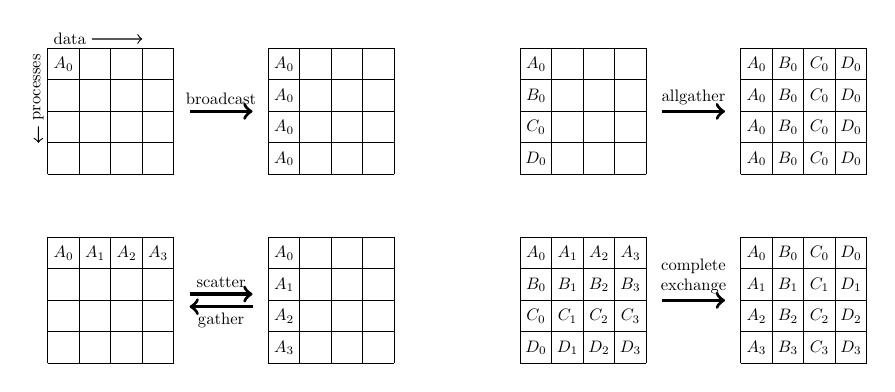
\begin{tikzpicture}[scale = 0.4, every node/.style={scale=0.6}]

\begin{scope}
	\begin{scope}
	\node[anchor = west] (Data) at (0, 4.3) {data};
	\node[anchor = east, rotate = 90] (Proc) at (-0.3, 4) {processes};
	\draw[->] (Data) -- (3, 4.3);
	\draw[->] (Proc) -- (-0.3, 1);
	\draw[step = 1cm] (0,0) grid (4,4);

	\node at (0.5, 3.5) {$A_0$};
	\end{scope}

	\draw[->, very thick] (4.5, 2) -- node[midway, above] {broadcast} (6.5, 2);

	\begin{scope}[xshift = 7cm]
	\draw[step = 1cm] (0,0) grid (4,4);

	\foreach \y in {0.5, 1.5, ..., 3.5}
		\node at (0.5, 4 - \y) {$A_0$};
	\end{scope}

	\begin{scope}[yshift = -6cm]
	\draw[step = 1cm] (0,0) grid (4,4);

	\foreach \x [count = \i from 0] in {0.5, 1.5, ..., 3.5}
		\node at (\x, 3.5) {$A_\i$};
	\end{scope}

	\draw[->, very thick] (4.5, -3.8) -- node[midway, above] {scatter} (6.5, -3.8);
	\draw[<-, very thick] (4.5, -4.2) -- node[midway, below] {gather} (6.5, -4.2);

	\begin{scope}[yshift = -6cm, xshift = 7cm]
	\draw[step = 1cm] (0,0) grid (4,4);

	\foreach \x [count = \i from 0] in {0.5, 1.5, ..., 3.5}
		\node at (0.5, 4 - \x) {$A_\i$};
	\end{scope}
\end{scope}

\begin{scope}[xshift = 15cm]
	\begin{scope}[yshift = 0cm]
	\draw[step = 1cm] (0,0) grid (4,4);

	\foreach \y/\l in {0.5/A, 1.5/B, 2.5/C, 3.5/D}
		\node at (0.5, 4 - \y) {$\l_0$};
	\end{scope}

	\draw[->, very thick] (4.5, 2) -- node[midway, above] {allgather} (6.5, 2);

	\begin{scope}[yshift = 0cm, xshift = 7cm]
	\draw[step = 1cm] (0,0) grid (4,4);

	\foreach \y in {0.5, 1.5, ..., 3.5} {
		\foreach \x/\l in {0.5/A, 1.5/B, 2.5/C, 3.5/D} {
			\node at (\x, 4 - \y) {$\l_0$};
		}
	}
	\end{scope}

	\begin{scope}[yshift = -6cm]
	\draw[step = 1cm] (0,0) grid (4,4);

	\foreach \y/\l in {0.5/A, 1.5/B, 2.5/C, 3.5/D} {
		\foreach \x[count = \i from 0] in {0.5, 1.5, ..., 3.5} {
			\node at (\x, 4 - \y) {$\l_\i$};
		}
	}
	\end{scope}

	\draw[->, very thick] (4.5, -4) -- node[midway, above, align = center] {complete \\ exchange} (6.5, -4);

	\begin{scope}[yshift = -6cm, xshift = 7cm]
	\draw[step = 1cm] (0,0) grid (4,4);

	\foreach \x/\l in {0.5/A, 1.5/B, 2.5/C, 3.5/D} {
		\foreach \y[count = \i from 0] in {0.5, 1.5, ..., 3.5} {
			\node at (\x, 4 - \y) {$\l_\i$};
		}
	}
	\end{scope}
\end{scope}

\end{tikzpicture}

\end{center}

\end{frame}


\begin{frame}[containsverbatim]
\frametitle{``v-version'' of \texttt{MPI$\_$Gather} : \texttt{MPI$\_$Gatherv}}
\begin{itemize}
	\item {adds a stride at receiving ends}
	\item {(example does not work if \texttt{stride > 100})}
\end{itemize}

\begin{center}
\input{Day3/images/gatherv.tex}
\end{center}

\end{frame}


\begin{frame}[containsverbatim]
\frametitle{``v-version'' of \texttt{MPI$\_$Gather} : \texttt{MPI$\_$Gatherv}}
\begin{lstlisting}[language=C,frame=lines]
MPI_Comm comm;
int gsize,sendarray[100];
int root, *rbuf, stride;
int *displs,i,*rcounts;
...
MPI_Comm_size(comm, &gsize);
rbuf = (int *)malloc(gsize*stride*sizeof(int));
displs = (int *)malloc(gsize*sizeof(int));
rcounts = (int *)malloc(gsize*sizeof(int));
for (i=0; i<gsize; ++i) {
   displs[i] = i*stride;
   rcounts[i] = 100;
}
MPI_Gatherv(sendarray, 100, MPI_INT, rbuf, rcounts, displs, MPI_INT,root, comm);
\end{lstlisting}
\end{frame}


\begin{frame}[containsverbatim]
\frametitle{``v-version'' of \texttt{MPI$\_$Scatter} : \texttt{MPI$\_$Scatterv}}
\begin{itemize}
	\item {adds a stride at sending ends}
	\item {(example does not work if \texttt{stride > 100})}
\end{itemize}

\begin{center}
% Slide 223
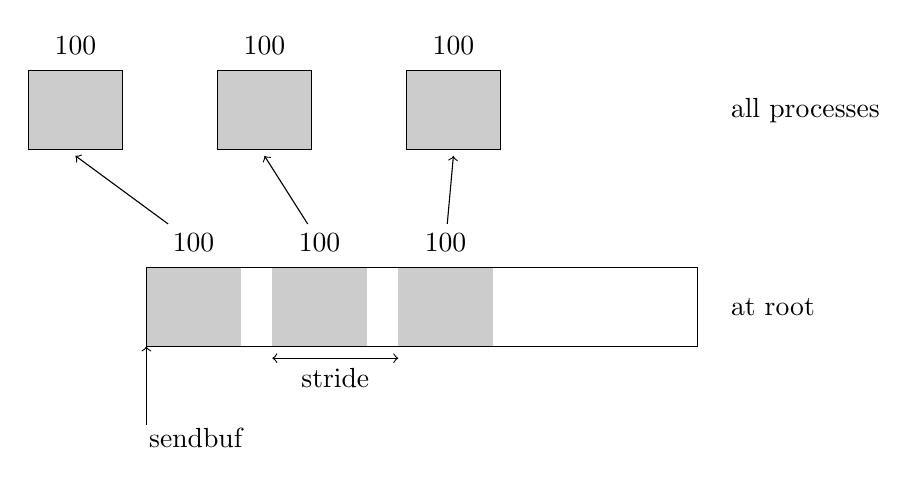
\begin{tikzpicture}

\foreach \x in {0, 1.6, 3.2} {
	\fill[gray!40!white] (\x, 0) rectangle (\x + 1.2, 1);
	\node[anchor = south] (N) at ({(2 * \x + 1.2)/ 2}, 1.08) {100};

	\pgfmathsetmacro{\xtop}{1.5 * (\x - 1)}
	\pgfmathsetmacro{\xmid}{(2 * \xtop + 1.2)/ 2}
	\draw[fill = gray!40!white] ({\xtop}, 2.5) rectangle ({\xtop + 1.2}, 3.5);
	\node[anchor = south] at (\xmid, 3.58) {100};

	\draw[->] (N) -- (\xmid, 2.42);
}

\draw (0,0) rectangle (7, 1);

\node[anchor = west] at (7.3, 0.5) {at root};
\node[anchor = west] at (7.3, 3) {all processes};

\node[anchor = north west, outer sep = 0pt, inner sep = 1pt] (S) at (0, -1) {sendbuf};
\draw[->] (S.north west) -- (0,0);

\draw[<->] (1.6, -0.15) -- node[midway, below] {stride} (3.2, -0.15);

\end{tikzpicture}

\end{center}

\end{frame}


\begin{frame}[containsverbatim]
\frametitle{``v-version'' of \texttt{MPI$\_$Scatter} : \texttt{MPI$\_$Scatterv}}
\begin{lstlisting}[language=C,frame=lines]
MPI_Comm comm;
int gsize,*sendbuf;
int root, rbuf[100], i, *displs, *scounts;
...
MPI_Comm_size(comm, &gsize);
sendbuf = (int *)malloc(gsize*stride*sizeof(int));
...
displs = (int *)malloc(gsize*sizeof(int));
scounts = (int *)malloc(gsize*sizeof(int));
for (i=0; i<gsize; ++i) {
   displs[i] = i*stride;
   scounts[i] = 100;
}
MPI_Scatterv(sendbuf, scounts, displs, MPI_INT, rbuf, 100, MPI_INT, root, comm);
\end{lstlisting}
\end{frame}




\subsection{Non-blocking collectives (NBC)}


\begin{frame}[containsverbatim]
\frametitle{Non-blocking collectives (NBC) for what ?}
\begin{itemize}
	\item{Same situations as for non-blocking point-to-point communications :
		\begin{itemize}
			\item {small message sizes}
			\item {enough computation to perform between start and end of the communication}
			\item {algorithm that authorizes to compute with a partial knowledge of the data}
		\end{itemize}
	}
%	\item{}
\end{itemize}
\end{frame}

\begin{frame}[containsverbatim]
\frametitle{Non-blocking collectives (NBC)}
\begin{itemize}
	\item{\verb+int MPI_Ibarrier(MPI_Comm comm,+\\\verb+MPI_Request *request)+ : NB version of \verb+MPI_Barrier()+}
	\item{\verb+int MPI_Ibcast(void* buffer, int count,+\\\verb+ MPI_Datatype datatype, int root,MPI_Comm comm, MPI_Request *request)+ : NB version of \verb+MPI_Bcast()+. Example :

\begin{lstlisting}[language=C,frame=lines]
MPI_Comm comm;
int array1[100], array2[100];
int root=0;
MPI_Request req;
...
MPI_Ibcast(array1, 100, MPI_INT, root, comm, &req);
compute(array2, 100);
MPI_Wait(&req, MPI_STATUS_IGNORE);
\end{lstlisting}
	}
\end{itemize}
\end{frame}


\begin{frame}[containsverbatim]
\frametitle{Non-blocking collectives (NBC)}
Scatter/Gather versions
\begin{itemize}
	\item{\verb+int MPI_Igather()+ : NB version of \verb+int MPI_Gather()+}
	\item{\verb+int MPI_Igatherv()+ : NB version of \verb+int MPI_Gatherv()+}
	\item{\verb+int MPI_Iscatter()+ : NB version of \verb+int MPI_Scatter()+}
	\item{\verb+int MPI_Iscatterv()+ : NB version of \verb+int MPI_Scatterv()+}
\end{itemize}
All Scatter/Gather versions
\begin{itemize}
	\item{\verb+int MPI_Iallgather()+ : NB version of \verb+int MPI_Allgather()+}
	\item{\verb+int MPI_Iallgatherv()+ : NB version of \verb+int MPI_Allgatherv()+}
\end{itemize}
\end{frame}


\begin{frame}[containsverbatim]
\frametitle{Non-blocking collectives (NBC)}
All to all
\begin{itemize}
	\item{\verb+int MPI_Ialltoall()+ : NB version of \verb+int MPI_Alltoall()+}
	\item{\verb+int MPI_Ialltoallv()+ : NB version of \verb+int MPI_Alltoallv()+}
	\item{\verb+int MPI_Ialltoallw()+ : NB version of \verb+int MPI_Alltoallw()+}
\end{itemize}
\end{frame}

\begin{frame}[containsverbatim]
\frametitle{Non-blocking collectives (NBC)}
Reduce
\begin{itemize}
	\item{\verb+int MPI_Ireduce()+ : NB version of \verb+int MPI_Reduce()+}
	\item{\verb+int MPI_Iallreduce()+ : NB version of \verb+int MPI_Allreduce()+}
	\item{\verb+int MPI_Ireduce_scatter_block()+ : NB version of \verb+int MPI_Reduce_scatter_block()+}
	\item{\verb+int MPI_Ireduce_scatter()+ : NB version of \verb+int MPI_Reduce_scatter()+}
\end{itemize}
Scan
\begin{itemize}
	\item{\verb+int MPI_Iscan()+ : NB version of \verb+int MPI_Scan()+}
	\item{\verb+int MPI_Iexscan+ : NB version of \verb+int MPI_Exscan+}
\end{itemize}
\end{frame}


%\subsection{Virtual topologies}
%
%\begin{frame}[containsverbatim]
%\frametitle{Virtual topology}
%\begin{itemize}
%	\item{The communication pattern of a set of processes can be represented by a graph}
%	\item{nodes are processes, edges are connections}
%	\item{MPI provides functions to create a user defined topology}
%\end{itemize}
%A simple example is the cartesian topology :
%\begin{lstlisting}[language=C,frame=lines]
%int MPI_Cart_create(MPI_Comm comm_old, int ndims, const int dims[], const int periods[], int reorder, MPI_Comm *comm_cart)
%\end{lstlisting}
%\end{frame}


%\begin{frame}[containsverbatim]
%\frametitle{Virtual topology cartesian example}
%\begin{center}
%% Slide 231

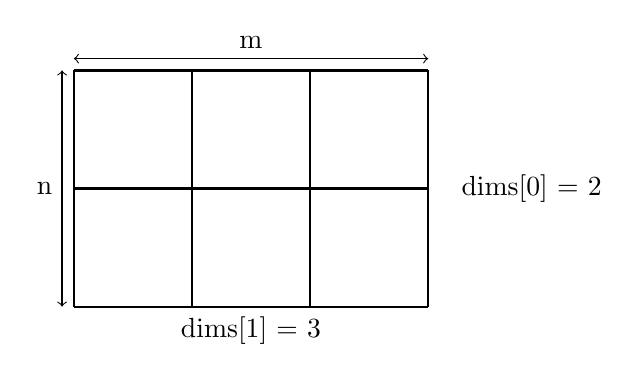
\begin{tikzpicture}

\draw[thick, step = 1.5cm] (0,0) grid (4.5, 3);
\node at (2.25, -0.3) {dims[1] = 3};
\node[anchor = west] at (4.8, 1.5) {dims[0] = 2};

\draw[<->, xshift = -0.15cm] (0,0) -- node[midway, left] {n} (0, 3);
\draw[<->, yshift = 0.15cm] (0,3) -- node[midway, above] {m} (4.5, 3);


\end{tikzpicture}

%\end{center}
%(source : Andrew Siegel, University of Chicago)
%\end{frame}


%\begin{frame}[containsverbatim]
%\frametitle{Virtual topology cartesian example}
%\begin{lstlisting}[language=C,frame=lines]
%gsizes[0] = m; // no. of rows in global array
%gsizes[1] = n; // no. of columns in global array
%psizes[0] = 2; // no. of procs. in vert. dimension
%psizes[1] = 3; // no. of procs. in hori. dimension
%lsizes[0] = m/psizes[0]; // no. of rows in local array
%lsizes[1] = n/psizes[1]; // no. of columns in local array
%dims[0] = 2; dims[1] = 3;
%periods[0] = periods[1] = 1;
%MPI_Cart_create(MPI_COMM_WORLD, 2, dims, periods, 0, &comm);
%\end{lstlisting}
%(source : Andrew Siegel, University of Chicago)
%\end{frame}

%\begin{frame}[containsverbatim]
%\frametitle{Generic virtual topologies}
%\begin{itemize}
%	\item{Operations on the new \verb+comm+ communicator : get the coordinates}
%\end{itemize}

%\begin{lstlisting}[language=C,frame=lines]
%MPI_Comm_rank(comm, &rank);
%MPI_Cart_coords(comm, rank, 2, coords);
%printf("Process %d has position (%d, %d) \n", rank, coords[0], coords[1]);
%\end{lstlisting}

%\begin{itemize}
%	\item{get a neighbor rank \verb+int MPI_Cart_shift(MPI_Comm comm,int direction,int displ,int *source,int *dest);+}
%\end{itemize}
%
%\begin{lstlisting}[language=C,frame=lines]
%MPI_Cart_shift(comm, 0, 1, &prank, &prank_south);
%\end{lstlisting}
%
%\end{frame}


\begin{frame}[containsverbatim]
\frametitle{Generic virtual topologies}
\begin{itemize}
	\item{despite MPI-1 provided functions to create general graph topology (\verb+int MPI_Graph_create()+), it was not scalable (all process needed to know the complete graph)}
	\item{MPI-2.2 introduce the \textit{distributed graph topology} : each process does not need to know the complete graph.}
	\item{\verb+int MPI_Dist_graph_create_adjacent()+ creates a new (local) communicator to which a topology information has been attached. Only adjacent processes. Example : stencil-based algorithm}
	\item{\verb+int MPI_Dist_graph_create()+ : create a new (local) communicator to which a topology has been attached (more general). }
\end{itemize}
\end{frame}

\begin{frame}[containsverbatim]
\frametitle{Generic virtual topologies}
\begin{itemize}
	\item{New collectives are then defined :
		\begin{itemize}
			\item{\verb+int MPI_Neighbor_alltoall+}
			\item{\verb+int MPI_Neighbor_allgather+}
			\item{...}
		\end{itemize}
}
\end{itemize}
\end{frame}




%\section{Hybrid programming}
%\subsection{Introduction}

\begin{frame}[containsverbatim]
	\frametitle{What will we learn today ?}	
	\begin{itemize}
		\item {Hybrid programming models comparison
			\begin{itemize}
				\item {Pure MPI}
				\item {MPI+OpenMP}
				\item {(MPI + MPI one-sided (MPI-3) )}
			\end{itemize}
		}
		\item {How to write a (production) project proposal}
	\end{itemize}
\end{frame}


\subsection{Hybrid programming models}


\begin{frame}[containsverbatim]
	\frametitle{Situation}	

\hspace*{2mm}% Slide 258
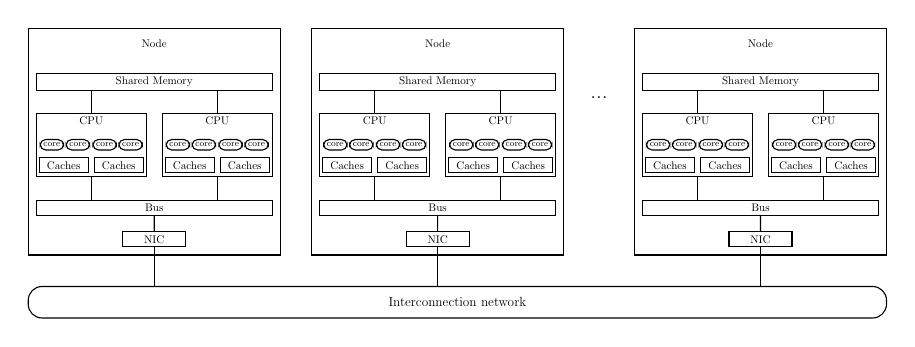
\begin{tikzpicture}[scale=0.4, every node/.style={scale=0.4}]

\pgfmathsetmacro{\lastxstart}{19}

\foreach \x[count = \i] in {-0.25, 8.75, \lastxstart} {
	\begin{scope}[xshift = \x cm]
	\draw (0.25,0) rectangle (8.25, 7.2);

	\node[draw, rectangle, minimum width = 2cm] (NIC\i) at (4.25, 0.5) {NIC};
	\node[draw, rectangle, minimum width = 7.5cm] (Bus) at (4.25, 1.5) {Bus};
	\node[draw, rectangle, minimum width = 7.5cm] (Shared) at (4.25, 5.5) {Shared Memory};
	\node at (4.25, 6.7) {Node};

	\begin{scope}[xshift = 2.25cm, yshift = -0.5cm]
	\node[rectangle, draw, minimum height = 2cm, minimum width = 3.5cm] (CPU1) at (0, 4) {};
	\node[below] at (CPU1.north) {CPU};

	\foreach \x in {-1.25, -0.425, 0.425, 1.25}
		\node[draw, rectangle, rounded corners = 2pt, inner sep = 3pt] at (\x, 4) {\footnotesize core};

	\foreach \x in {0.875, -0.875}
		\node[draw, rectangle, minimum width = 1.55cm] at (\x, 3.35) {Caches};
	\end{scope}

	\begin{scope}[xshift = 6.25cm, yshift = -0.5cm]
	\node[rectangle, draw, minimum height = 2cm, minimum width = 3.5cm] (CPU2) at (0, 4) {};
	\node[below] at (CPU2.north) {CPU};

	\foreach \x in {-1.25, -0.425, 0.425, 1.25}
		\node[draw, rectangle, rounded corners = 2pt, inner sep = 3pt] at (\x, 4) {\footnotesize core};

	\foreach \x in {0.875, -0.875}
		\node[draw, rectangle, minimum width = 1.55cm] at (\x, 3.35) {Caches};
	\end{scope}

	\draw (CPU1 |- Shared.south) -| (CPU1.north);
	\draw (CPU2 |- Shared.south) -| (CPU2.north);

	\draw (CPU1 |- Bus.north) -| (CPU1.south);
	\draw (CPU2 |- Bus.north) -| (CPU2.south);

	\draw (Bus) -- (NIC\i);
	\end{scope}
}

\pgfmathsetmacro{\lastx}{\lastxstart + 8.25}

\node[draw, rectangle, rounded corners = 5pt, minimum width = \lastx cm, minimum height = 1cm] (ICN) at ({\lastx / 2}, -1.5) {\large Interconnection network};

\draw (NIC1 |- ICN.north) -| (NIC1.south);
\draw (NIC2 |- ICN.north) -| (NIC2.south);
\draw (NIC3 |- ICN.north) -| (NIC3.south);

\node at (18.125, 5) {\huge ...};

\end{tikzpicture}


\end{frame}



\begin{frame}[containsverbatim]
	\frametitle{Situation}	

\vspace*{2mm}\input{Day4/images/situation-openmp-mpi.tex}

\end{frame}

\begin{frame}[containsverbatim]
	\frametitle{Situation : problems}	
\begin{itemize}
	\item {Thread safety ?}
	\item {Which thread/process can/will call the MPI library ?}
	\item {MPI process placement in the case of multi-CPU processors ?}
	\item {Data visibility ? OpenMP private ? }
	\item {Does my problem fits with the targeted machine ?}
	\item {Levels of parallelism within my problem ?}
\end{itemize}
\end{frame}



\begin{frame}[containsverbatim]
	\frametitle{Hybrid vs. Pure MPI}	
\textbf{Pure MPI}
\begin{itemize}
	\item {\textbf{+} no code modification}
	\item {\textbf{+} most of the libraries support multi-thread}
	\item {\textbf{-} does application topology fits system topology ?}
	\item {\textbf{-} useless communications}
\end{itemize}
\textbf{Hybrid}
\begin{itemize}
	\item {\textbf{+} no message within an SMP node}
	\item {\textbf{+} less (no) topology problems}
	\item {\textbf{-} all threads sleep when master communicates}
	\item {\textbf{-} MPI-libs must support (at least) thread safety}
\end{itemize}
\end{frame}


\begin{frame}[containsverbatim]
\frametitle{Hybrid MPI/OpenMP hello world}
\begin{lstlisting}[language=C,frame=lines]
int main(int argc, char *argv[]) {
  int numprocs, rank, namelen,provided;
  char processor_name[MPI_MAX_PROCESSOR_NAME];
  int iam = 0, np = 1;
  MPI_Init_thread(&argc, &argv,MPI_THREAD_SINGLE,provided);
  MPI_Comm_size(MPI_COMM_WORLD, &numprocs);
  MPI_Comm_rank(MPI_COMM_WORLD, &rank);
  #pragma omp parallel default(shared) private(iam, np)
  {
    np = omp_get_num_threads();
    iam = omp_get_thread_num();
    printf("Hello from thread %d out of %d from process %d out of %d on\n",iam, np, rank, numprocs);
  }
  MPI_Finalize();
}
\end{lstlisting}

Need to overlap communications (from master) with computation between the others. If possible !

\end{frame}



\begin{frame}[containsverbatim]
\frametitle{Hybrid MPI/OpenMP hello world}

  Compilation using the GNU gcc compiler:
\begin{verbatim}
mpicc -fopenmp hello.c -o hello
\end{verbatim}
  Compilation using the Intel C compiler:

\begin{verbatim}
mpiicc -qopenmp hello.c -o hello
\end{verbatim}

Warning : when using Intel MPI : it is mandatory to link against the thread-safe library (-mt$\_$mpi) or at least to check if the executable has been linked against this lib (\verb+ldd hello+ should print \verb+libmpi_mt.so.XX+) if \verb+mpiicc+ or \verb+mpiifort+ has been used.

\end{frame}


\begin{frame}[containsverbatim]
\frametitle{Submission script the clusters}

\begin{verbatim}
#!/bin/bash
#SBATCH --nodes 2
#SBATCH --ntasks 2
#SBATCH --cpus-per-task 16
#SBATCH --ntasks-per-node=1
#SBATCH --time 00:00:30
#SBATCH --workdir /scratch/vkeller

module purge
module load intel intel-mpi

export OMP_NUM_THREADS=$SLURM_CPUS_PER_TASK
srun ./hello 
\end{verbatim}

It will start 2 MPI processes each will spawn 16 threads

\end{frame}













\begin{frame}[fragile]
\frametitle{Changes to your code}
\begin{itemize}
\item change your MPI initialisation routine
\begin{itemize}
    \item \verb+MPI_Init+ is replaced by \verb+MPI_Init_thread+
    \item \verb+MPI_Init_thread+ has two additional parameters for the level of thread support
        required, and for the level of thread support provided by the library implementation
\end{itemize}

\begin{Verbatim}[formatcom=\color{blue}]
int MPI_Init_thread(int *argc, char ***argv, 
                      int required, int *provided)
\end{Verbatim}

       \textcolor{dkgreen}{required specifies       the     requested       level   of      thread  support,        and     the     actual  level   of      support is      then    returned        into    provided}

\item add OpenMP directives or Pthread calls as long as you stick to the level of thread safety you specified in the call to \verb+MPI_Init_thread+
\end{itemize}

\end{frame}


\begin{frame}[fragile]
\frametitle{The 4 Options for Thread Support}
%\framesubtitle{I: user informs the MPI library}


\begin{itemize}
\item \verb+MPI_THREAD_SINGLE+
\begin{itemize}
\item Only one thread will execute
\item Standard MPI-only application
\end{itemize}
\item \verb+MPI_THREAD_FUNNELED+
\begin{itemize}
\item Only the Master Thread will make calls to the MPI library
%\item $\rightarrow$ The thread that calls \verb+MPI_Init_thread+ is the master thread
\item A thread can determine whether it is the master thread by a call to \verb+MPI_Is_thread_main+
\end{itemize}
\item \verb+MPI_THREAD_SERIALIZED+
\begin{itemize}
\item Only one thread at a time will make calls to the MPI library, but all threads are eligible to make such calls
\end{itemize}
\end{itemize}

%\begin{Verbatim}[formatcom=\color{blue}]
%int MPI_Is_main_thread(int * flag);
%\end{Verbatim}
\end{frame}


\begin{frame}[fragile]
\frametitle{The 4 Options for Thread Support}
%\framesubtitle{II: The MPI Library is responsible for Thread Safety}

\begin{itemize}
\item \verb+MPI_THREAD_MULTIPLE+
\begin{itemize}
\item Any thread may call the MPI library at any time
\item The MPI library is responsible  for thread safety within that library, and for any libraries that  it in turn uses
\item Codes that rely on the level of \verb+MPI_THREAD_MULTIPLE+ may run significantly slower than the  case where one of the other options has been chosen
\item You might need to link in a separate library in order to get this level of support
\end{itemize}
\end{itemize}


    In  most    cases   \verb+MPI_THREAD_FUNNELED+      provides        the     best    choice  for     hybrid  programs

\begin{Verbatim}[formatcom=\color{blue}]
int MPI_Query_thread( int * thread_level_provided);
\end{Verbatim}

Returns the level of thread support provided by the MPI library

\end{frame}



\begin{frame}
\frametitle{Topology problems}

%The problem: we have a domain with 80 subdomains as follows:
%
%\begin{center}
%\begin{tikzpicture}%
%  \draw[step=4mm] (0,0) grid (6.4,2.0);
%\end{tikzpicture}
%\end{center}

How to deal with :

\begin{itemize}
\item topology / mapping ? (Which physical core is assigned to which process/thread)
\item sub-domain decomposition ?
\item halos size ? halos shapes ?
\item unnecessary communications ?
\item \textbf{computation to communication ratio} ?
\end{itemize}

Pure MPI ? Hybrid ?
\\
\textbf{A good solution is : one MPI process per ``SMP'' node}

\end{frame}



\begin{frame}
\frametitle{Halo regions}
% Neil, p. 54
\begin{itemize}
\item  Halo regions are local copies of remote data that are needed for computations
\item  Halo regions need to be copied fequently
\item  Using threads reduces the size of halo region copies that need to be stored
\item  Reducing halo region sizes also reduces communication requirements
\end{itemize}
\end{frame}



\begin{frame}
\frametitle{Take-home messages}
\begin{itemize}
\item Always take into account the problems related to the physical topology
\item A real application is not as easy as a hello world.
\item Some clusters have different connectivity topologies: match them to your problem. Examples of hardware topologies :
\begin{itemize}
\item all-to-all
\item 2D/3D torus
\item tree
\item ...
\end{itemize}
        \item One MPI process per physical node 
\end{itemize}
\end{frame}





\begin{frame}[fragile]
\frametitle{Main messages}
\begin{itemize}
\item Do not use hybrid if the pure MPI code scales ok
\item Be aware of intranode MPI behavior
\item Always observe the topology dependence of
\begin{itemize}
   \item Intranode MPI
   \item Threads overheads
\end{itemize}
\item Finally: Always compare the best pure MPI code with the best hybrid code!
\end{itemize}

\end{frame}


\begin{frame}[fragile]
\frametitle{Examples that \textit{can} benefit of an hybrid approach}
\begin{itemize}
\item MPI codes with a lot of all-to-all communications
\item MPI codes with a very poor load balancing at the algorithmic level (less communications)
\item MPI codes with memory limitations
\item MPI codes that can be easily \textit{fine-grained parallelized} (at loop level)
\item MPI codes that will offload codes on accelerators
\end{itemize}

\end{frame}





%%% Local Variables: 
%%% mode: latex
%%% TeX-master: "../cours_vince"
%%% End: 


%\section{Project proposals propositions}
%\begin{frame}[containsverbatim]
\begin{center}
\textbf{How to write a project proposal ?}
\end{center}
\end{frame}

\subsection{How to write a project proposal}

\begin{frame}[containsverbatim]
	\frametitle{Structure of a (good) project proposal}	

\begin{itemize}
	\item{(Administration) Who submits it ?}
	\item{(Scientific : Background) From where do we come ?}
	\item{(Scientific : Outcome) Where do we go ?}
	\item{(Technical : Application) What do we  have, how it is implemented ?}
	\item{(Technical : Performance) Why do we need a high-end machine ?}
	\item{(Technical : Resource budget) How much do we need ?}
\end{itemize}

\end{frame}



\subsection{Administrative stuff}

\begin{frame}[containsverbatim]
	\frametitle{Project title}

\begin{itemize}
	\item {Keep it as explicit as possible}
	\item {Propose an accronym (8 letters) : often used as group name}
	\item {Follow the Computing Center's rules}
	\item{\textcolor{dkgreen}{\textit{A High Performance Implementation of a 2D Elliptic Equation Solver: the Poisson's Equation Case at Scale}. Acronym : POISSON} }
	\item{\textcolor{dkred}{\textit{Implementation of a Generic Poisson Solver}. Acronym : POISSON} }
\end{itemize}


\end{frame}



\begin{frame}[containsverbatim]
	\frametitle{Intro cartouche}

The goal is to have the basic administrative stuff and the main requests at a first glance

\begin{center}
\begin{tabular}{| l | l |}
	\hline
	Principal investigator & Vincent Keller, PhD \\
	\hline
	Institution & \'Ecole Polytechnique F\'ed\'erale de Lausanne \\
	\hline
	Laboratory & Scientific IT and Application Support \\
	\hline
	Adress & Station 1, CH-1015 LAUSANNE \\
	\hline
	Involved researchers & Nicolas Richart, PhD ; Christian Cl\'emen\c{c}on \\
	\hline
	Date of submission & April 13, 2015 \\
	\hline
	Expected end of project & October 13, 2015 \\
	\hline
	Target machine & CADMOS Blue Gene Q \\
	\hline
	Proposed acronym & ACRO \\
	\hline
\end{tabular}
\end{center}
\end{frame}


\subsubsection{PI, involved people, institution, CV's}


\begin{frame}[containsverbatim]
	\frametitle{Intro cartouche : Good / Bad practices}

\begin{itemize}
	\item{\textcolor{dkgreen}{Keep it as short as possible}}
	\item{\textcolor{dkgreen}{PI + Key personnel, institution(s), start/end of project, summary of the technical request}}
	\item{\textcolor{dkred}{Not too many details}}
	\item{\textcolor{dkred}{CVs of the project members (put them in an approriate appendix)}}
	\item{\textcolor{dkred}{Potential Collaborations}}
\end{itemize}
\end{frame}



\subsection{Scientific background}

\begin{frame}[containsverbatim]
	\frametitle{Scientific background}
\begin{itemize}
	\item{\textbf{Most important section of the proposal}}
	\item{You and your fellow research scientists or engineers are aware if your research deserves to get computing power}
	\item{To help you : 
	\begin{itemize}
		\item{Good abstract}
		\item{Description of the project}
		\item{References}
	\end{itemize}
	}
%	\item{}
\end{itemize}
\end{frame}


\subsubsection{Abstract}

\begin{frame}[containsverbatim]
	\frametitle{Abstract}

\begin{itemize}
	\item{\textcolor{dkgreen}{ Explicitly express the link between the scientific background and the technical request}}
	\item{\textcolor{dkgreen}{ 500 words max. } }
	\item{\textcolor{dkgreen}{ Assume the reader has little/no knowledge about the technical part and/or the scientific matter} }
	
	\item{\textcolor{dkred}{No copy/paste from previous publications}}
%	\item{\textcolor{red}{}}
%	\item{\textcolor{red}{}}
%	\item{\textcolor{red}{}}
\end{itemize}
\end{frame}


\subsubsection{Description of the project}

\begin{frame}[containsverbatim]
	\frametitle{Description of the project}

\begin{itemize}
	\item{\textcolor{dkgreen}{Description of the research/production project} }
	\item{\textcolor{dkgreen}{Motivation}
		\begin{itemize}
			\item{My project uses an existing, known and well-tested code (Production project)}
			\item{My project will explore a new paradigm at scale (exploratory project)}
			\item{My project has never been tested at scale, needs improvements from an existing code (research project)}
		\end{itemize}
	}
	\item{\textcolor{dkgreen}{Computational objectives} }
	\item{\textcolor{dkgreen}{Expected innovations both at scientific and computational levels} }
%	\item{\textcolor{red}{}}
%	\item{\textcolor{red}{}}
%	\item{\textcolor{red}{}}
\end{itemize}
\end{frame}


\begin{frame}[containsverbatim]
	\frametitle{Scientific background and outcome}
\textbf{Most important point : this part is usually peer-reviewed by a pool of experts/reviewers from the domain.}
\begin{itemize}
	\item{\textcolor{dkgreen}{State-of-the-art review} }
	\item{\textcolor{dkgreen}{Extensive references} }
	\item{\textcolor{dkgreen}{Current status on the subject}	} 
	\item{\textcolor{dkred}{``We are the only ones in the world doing that and you are too stupid to understand it''} }
%	\item{\textcolor{red}{}}
%	\item{\textcolor{red}{}}
%	\item{\textcolor{red}{}}
\end{itemize}
\end{frame}



\subsection{Technical part}

\begin{frame}[containsverbatim]
	\frametitle{Technical part}

Technical part of the project proposal. What is the \textbf{application} you are planning to run on the target architecture ?

\begin{itemize}
	\item{What code (application) are we planning to use }
	\item{Numerical methods
		\begin{itemize}
			\item{ FEM, SEM, FDM, LBM, SPH, MD, etc..}
		\end{itemize}
	}
	\item{Algorithms
		\begin{itemize}
			\item{ Describe the main algorithms}
			\item{ Main bottlenecks and how they have been tackled}
		\end{itemize}
	}
	\item{Implementation 
		\begin{itemize}
			\item{ Pure MPI, GPU, OpenMP, hybrid ? ...}
			\item{ Does it use special libraries ? }
		\end{itemize}
	}
	\item{If third-party code : name, version and license. Your contact within the third-party company/institution}
\end{itemize}
\end{frame}





\subsection{Performance}


\begin{frame}[containsverbatim]
	\frametitle{Performance expectations}

This section should explain how your code behaves and the accuracy with what you request.

\begin{itemize}
	\item { theoretical complexity: communication and computation complexities }
	\item { weak scaling : behavior of the application by fixing the size of the problem per processor and increasing the number of processors: \textbf{parallel efficiency} ($E_p = S_p/p$) }
	\item { strong scaling : behavior of the application by fixing the total size of the problem and increasing the number of processors: \textbf{speedup} ($S_p = t_1/t_p$) }
\end{itemize}
\end{frame}


\subsubsection{Theoretical complexity}


\begin{frame}[containsverbatim]
	\frametitle{Benchmarking}


\begin{itemize}
	\item { You get access to a \textbf{test partition} which allows you to run test cases and measure the performance }
	\item { You also have previous performance measurements from the development }
	\item { Benchmarking is done on larger enough problems, closer to what will be done in production }
	\item { Use the theoretical complexities (computation and communication) to predict how your application will behave at production scale }
\end{itemize}
\end{frame}



\subsubsection{Strong scaling}


\begin{frame}[containsverbatim]
	\frametitle{Strong scaling : Good example (with speedup)}

\begin{columns}
\column{0.5\textwidth} %first column
\begin{center}
\includegraphics[width=5cm]{Day4/images/strong-good2.png}
\end{center}

\column{0.5\textwidth} %second column
\begin{itemize}
	\item {log-log graph}
	\item {Different problem sizes}
	\item {linear regression curves}
\end{itemize}
\end{columns}
\textbf{Source: HLRS \url{http://inside.hlrs.de/_old/htm/Edition_01_12/article_20.html}}

\end{frame}


\begin{frame}[containsverbatim]
	\frametitle{Strong scaling : Good example (with timing)}

\begin{columns}
\column{0.5\textwidth} %first column
\begin{center}
\includegraphics[width=6cm]{Day4/images/strong-good.png}
\end{center}

\column{0.5\textwidth} %second column
\begin{itemize}
	\item {log-log graph}
	\item {time \textbf{per step}}
	\item {explicit caption}
	\item {linear regression curves}
\end{itemize}
\end{columns}
\textbf{Source: CRPP, EPFL, Project proposal for BG/P, 2011}

\end{frame}


\begin{frame}[containsverbatim]
	\frametitle{Strong scaling : bad example}

\begin{columns}
\column{0.5\textwidth} %first column
\begin{center}
\includegraphics[width=5cm]{Day4/images/strong-bad.png}
\end{center}

\column{0.5\textwidth} %second column
\begin{itemize}
	\item {linear scale}
	\item {no caption}
	\item {``Excel'' look}
	\item {useless for any conclusion}
\end{itemize}
\end{columns}

\end{frame}


\subsubsection{Weak scaling}

\begin{frame}[containsverbatim]
	\frametitle{Weak scaling : Good example (FZJ J\"ulich, Germany)}

\begin{columns}
\column{0.5\textwidth} %first column
\begin{center}
\includegraphics[width=6cm]{Day4/images/weak-good.png}
\end{center}

\column{0.5\textwidth} %second column
\begin{itemize}
	\item {log-log graph}
	\item {runtimes and efficiency on the same graph}
	\item {two different problem sizes}
	\item {complexity order clearly stated}
	\item {Prediction on the largest partition of JUQUEEN}
\end{itemize}
\end{columns}

\textbf{Source: Performance of PEPC \url{http://www.fz-juelich.de/ias/jsc/EN/AboutUs/Organisation/ComputationalScience/Simlabs/slpp/SoftwarePEPC/_node.html}}

\end{frame}



\begin{frame}[containsverbatim]
	\frametitle{Weak scaling : bad example}

\begin{columns}
\column{0.5\textwidth} %first column
\begin{center}
\includegraphics[width=7cm]{Day4/images/weak-bad.png}
\end{center}

\column{0.5\textwidth} %second column
\begin{itemize}
	\item {linear scales}
	\item {no caption}
	\item {``Excel'' look}
	\item {comparison between CPUs and GPUs on the same graph? What is the ``best''? Data does not fit in GPU memory, then?}
\end{itemize}
\end{columns}

\end{frame}



\subsection{Resource budget}


\begin{frame}[containsverbatim]
	\frametitle{Resource budget}

Based on the performance expectations and benchmarks already done, you are able to provide a resource budget for your proposal

\begin{itemize}
	\item { Typical size of problem to solve. Total number of problems to solve }
	\item { Minimum and maximum memory size for the problems }
	\item { Disk space }
	\item { Communications needs (paradigm choice) }
	\item { Architecture }
\end{itemize}
\end{frame}





\begin{frame}[containsverbatim]
	\frametitle{Summary of the Resource Budget}
For the targeted problems
\begin{center}
\begin{tabular}{| l | l |}
	\hline
	Total number of requested cores & 128 - 512 [cores]\\
	\hline
	Minimum total memory & 10 [GB] \\
	\hline
	Maximum total memory & 256 [GB] \\
	\hline
	Temporary disk space for a single run & 100 [GB] \\
	\hline
	Permanent disk space for the entire project & 1 [TB] \\
	\hline
	Communications & Pure MPI \\
	\hline
	License & own code (BSD) \\
	\hline
	Code publicly available ? & Yes \\
	\hline
	Library requirements & LAPACK \\
	\hline
	Architectures where code ran & Intel 64, BG/Q  \\
	\hline
\end{tabular}
\end{center}
\end{frame}



\subsection{Facultative}


\begin{frame}[containsverbatim]
	\frametitle{Facultative add-ons}

\begin{itemize}
	\item { Technical support from the Computing Center (CC)}
	\item { Application-level support from the CC or other institution/groups}
\end{itemize}
\end{frame}








%%%%%%%%%%%%%%%%%%%%%%%%%%%%%%%%%%%%%%
% Pour le cours PHPC
%%%%%%%%%%%%%%%%%%%%%%%%%%%%%%%%%%%%%%

%\section{Projects}
%\subsection{Introduction}
\begin{frame}[containsverbatim]
\frametitle{Parallelization mini-projects}

\begin{itemize}
	\item{60 hours of personal work}
	\item{Individual (for some hard problems : binom)}
	\item{We propose subjects but \textbf{you can propose yours !}}
	\item{MPI or CUDA (OpenMP/hybrid/MPI-IO are a plus)}
\end{itemize}

%\begin{alertblock}{Blabla}
%\begin{alertblock}{Blabla}
%\begin{block}{Blabla}
%\end{block}

Important dates :

\begin{center}
\begin{tabular}{ | l | l |}
\hline
\textbf{Deliverable} & \textbf{Due date} \\
\hline
Fixing topic & May 2, 2016 \\
\hline
Theoretical Analysis & May 15, 2016 \\
\hline
Final Report & June 5, 2016 \\
\hline
Exam (15' pres + 15' Q\&A) & June 23, 2016 8:15-18:00 \\
&and June 24, 2016 8:15-18:00 \\
\hline
\end{tabular}	
\end{center}

(all at 11:59 pm. CEST)

\end{frame}




\subsection{Julia set}
\begin{frame}[containsverbatim]
\frametitle{Julia set}
\begin{center}
\includegraphics[width=5.0cm]{Day2/images/julia2.png}
\end{center}
\begin{block}{Problem description}
The Julia set is the set of points of the complex plan $z = a + b i$ such that the suite
$$
z_{(n+1)} = z_n^2 + c
$$
remains bounded when $n \rightarrow \infty$. $c$ is a constant. 
\end{block}
\end{frame}
\begin{frame}[containsverbatim]
\frametitle{Julia set}
\begin{block}{Important remarks}
\begin{itemize}
	\item{load balancing}
\end{itemize}
\end{block}
\end{frame}



\subsection{Mandelbrot set}
\begin{frame}[containsverbatim]
\frametitle{Mandelbrodt set}
\begin{center}
\includegraphics[width=3.0cm]{Day2/images/mandelbrot.jpg}
\end{center}
\begin{block}{Problem description}
The Mandelbrot set is the set of complex numbers $c$ obtained by the quadratic recurrence equation :
$$
\left\{ \begin{array}{r}
 z_0 = 0 \\
  z_{(n+1)} = z_n^2 + c
       \end{array} \right.
$$
such the suite does not diverge when $n \rightarrow \infty$. 
\end{block}
\end{frame}
\begin{frame}[containsverbatim]
\frametitle{Mandelbrodt set}
\begin{block}{Important remarks}
\begin{itemize}
	\item{load balancing}
	\item{a \textit{colored plot} is obtained by coloring the points with the number of steps required to reach the cut-off value $r_{max}$ value (usually $r_{max} = 2$)}
	\item{Mandelbrot set is considered as a ``map'' of all the Julia sets because it uses a different $c$ at each $z$.}
\end{itemize}
\end{block}
\end{frame}




\subsection{Traveling Salesman Problem}
\begin{frame}[containsverbatim]
\frametitle{Traveling Salesman Problem}
\begin{center}
\includegraphics[width=4.0cm]{Day2/images/tsp.png}
\\
{\tiny Figure credit: David Applegate, Robert Bixby, Vasek Chvatal and William Cook.}
\end{center}
\begin{block}{Problem description}
Let us have an undirected weighted graph where : cities are the vertices, the edges are the paths, the weight a distance between two cities. The TSP solution is the shortest path starting and finishing at the same vertice and by visiting all the other vertices one and only one time.
\end{block}
\end{frame}
\begin{frame}[containsverbatim]
\frametitle{Traveling Salesman Problem}
\begin{block}{Important remarks}
\begin{itemize}
	\item{load balancing}
	\item{tree construction}
\end{itemize}
\end{block}
\end{frame}




\subsection{N-queens problem}
\begin{frame}[containsverbatim]
\frametitle{N queens problem}
\begin{center}
\includegraphics[width=4.0cm]{Day2/images/queen.jpg}
\end{center}
\begin{block}{Problem description}
The N-queens problem is the problem of placing $N$ queens on an $N \times N$ board ($N>3$) so that no queen see each other. A queen can move on its row, its column and its diagonals.
\end{block}
\end{frame}
%\begin{frame}[containsverbatim]
%\frametitle{n queens problem}
%\begin{block}{Important remarks}
%\begin{itemize}
%	\item{tree construction}
%	\item{}
%\end{itemize}
%\end{block}
%\end{frame}




\subsection{FFT}
\begin{frame}[containsverbatim]
\frametitle{FFT with Cooley-Tukey}
\begin{center}
\includegraphics[width=4.0cm]{Day2/images/fft.png}
\end{center}
\begin{block}{Problem description}
The Fast Fourier Transform (FFT) Cooley-Tukey algorithm computes the Discrete Fourier Transform (DFT) of a sequence recursively by a devide-and-conquer approach. The radix-2 decimation in time divides a DFT of size $N$ into two interleaved DFT of size $N/2$.
\end{block}
\end{frame}
%\begin{frame}[containsverbatim]
%\frametitle{FFT with Cooley-Tukey}
%A DFT is described as :
%$$
%X_k = \sum_{n=0}^{N-1} x_n e^{- \frac{2 \pi i}{N} n k}
%$$
%which can be rearranged as :
%$$
%X_k = \sum_{m=0}^{N/2-1} x_{2m} e^{- \frac{2 \pi i}{N/2} (2m) k} + e^{- \frac{2 \pi i}{N} k} \sum_{m=0}^{N/2-1} x_{2m+1} e^{- \frac{2 \pi i}{N/2} m k}
%$$
%in other words : the even and the odd parts of $X_k$ :
%$$
%X_k = E_k + e^{- \frac{2 \pi i}{N}k} O_k
%$$
%\end{frame}
%\begin{frame}[containsverbatim]
%\frametitle{FFT with Cooley-Tukey}
%Therefore:
%$$
%X_k = \left\{ \begin{array}{ll}
% E_k + e^{- \frac{2 \pi i}{N/2}k} O_k & \text{for}~~ 0 \leq k < N/2\\
%  E_{k-N/2} + e^{- \frac{2 \pi i}{N/2}k} O_{k-N/2} &\text{for}~~ N/2 \leq k < N.
%       \end{array} \right.
%$$
%we also know that :
%$$
%e^{- \frac{2 \pi i}{N}(k+ N/2)} = - e^{- \frac{2 \pi i}{N}k}
%$$
%thus for $0 \leq k < \frac{N}{2}$ :
%$$
%\begin{array}{ll}
%X_k & = E_k + e^{- \frac{2 \pi i}{N}k} O_k \\
%X_{k+\frac{N}{2}} & = E_k - e^{- \frac{2 \pi i}{N}k} O_k
%\end{array}
%$$
%\end{frame}
%\begin{frame}[containsverbatim]
%\frametitle{FFT with Cooley-Tukey}
%The DFT of length $N$ is then described in terms of two DFT of size $\frac{N}{2}$. The same process is applied recursively until $N=2$.
%\end{frame}
\begin{frame}[containsverbatim]
\frametitle{FFT with Cooley-Tukey}
\begin{block}{Important remarks}
\begin{itemize}
	\item{Complexity !}
	\item{$x_k$ reordering before devide-and-conquer}
	\item{Large size numbers $N = 2^t$ with $t$ as ``large'' as possible}
	\item{You can choose other algorithms than Cooley-Tukey}
\end{itemize}
\end{block}
\end{frame}




\subsection{Minimum spanning tree}
\begin{frame}[containsverbatim]
\frametitle{Minimum Spanning Tree}
\begin{center}
\includegraphics[width=4.0cm]{Day2/images/spanning.png}
\end{center}
\begin{block}{Problem description}
A minimum spanning tree is a spanning tree of a connected, undirected and weighted graph. It connects all the vertices together with the minimal total weighting for its edges
\end{block}
\end{frame}
\begin{frame}[containsverbatim]
\frametitle{Minimum Spanning Tree}
\begin{block}{Important remarks}
\begin{itemize}
	\item{Parallelize Boruka's algorithm}
	\item{Complexity !}
\end{itemize}
\end{block}
\end{frame}




\subsection{Dijkstra's algorithm}
\begin{frame}[containsverbatim]
\frametitle{Dijkstra's algorithm}
\begin{center}
\includegraphics[width=4.0cm]{Day2/images/dijkstras.png}
\end{center}
\begin{block}{Problem description}
Dijkstra's algorithm is an algorithm for finding the shortest paths between nodes in a graph. It can be used for finding the shortest paths from a single node to a single destination node by stopping the algorithm once the shortest path to the destination node has been determined
\end{block}
\end{frame}
%\begin{frame}[containsverbatim]
%\frametitle{Dijkstra's algorithm}
%\begin{block}{Important remarks}
%\begin{itemize}
%	\item{parallelization of the tree}
%\end{itemize}
%\end{block}
%\end{frame}





\subsection{N-body simulation}
\begin{frame}[containsverbatim]
\frametitle{N-body simulation}
\begin{center}
\includegraphics[width=3.0cm]{Day2/images/nbody.png}
\end{center}
\begin{block}{Problem description}
The n-body problem aims at simulating a dynamical system of particles under the influence of physical forces. We'll restrain on the gravity field applied on celestial bodies:
$$
F_{ij} = \frac{G m_i m_j (q_j - q_i)}{||q_j - q_i||}
$$
where $G$ is the gravitational constant, $m_i$ and $m_j$ the masses of the $i$-th and $j$-th bodies and $q_i$ and $q_j$ their positions.
\end{block}
\end{frame}
\begin{frame}[containsverbatim]
\frametitle{N-body simulation}
\begin{block}{Important remarks}
\begin{itemize}
	\item{brute force will not be accepted}
	\item{2D or 3D}
	\item{non-uniform initial distribution must be tested to stress the application}
	\item{how to handle collisions and ``lost bodies in the far space''}
\end{itemize}
\end{block}
\end{frame}



\subsection{Sieve of Eratosthenes}
\begin{frame}[containsverbatim]
\frametitle{Sieve of Eratosthenes}
\begin{center}
\includegraphics[width=3.0cm]{Day2/images/Eratosthene.png}
\end{center}
\begin{block}{Problem description}
Find all the prime numbers $p$ such $p < N$ where $N$ is very large. Enumerate all the multiples of $p$ by counting to $N$ in incerements of $p$ and mark them as ``non-primes''. Do that to $\sqrt{N}$. The list of $p_i$ are all the primes between $p=2$ to $p=\sqrt{N}$.
\end{block}
\end{frame}
\begin{frame}[containsverbatim]
\frametitle{Sieve of Eratosthenes}
\begin{block}{Important remarks}
\begin{itemize}
	\item{load balancing}
	\item{Handling very large numbers}
	\item{alternative : Sieve of Atkin}
\end{itemize}
\end{block}
\end{frame}





\subsection{Game of Life}
\begin{frame}[containsverbatim]
\frametitle{Game of Life}
\begin{center}
\includegraphics[width=3.0cm]{Day2/images/gameoflife.png}
\end{center}
\begin{block}{Problem description}
The game of life is a cellular automaton with simple elements: a cell $c_i$ can be dead ($c_i = 0$) or alive ($c_i = 1$). At each time step, the following rules are applied :
\begin{itemize}
	\item {if $c_i = 1$ and its neighbours are 0, 1 or 4 living cells, then $c_{i+1} = 0$}
	\item {if $c_i = 1$ and its neighbours are 2 or 3 living cells, then $c_{i+1} = 1$}
	\item {if $c_i = 0$ and its neighbours are exactly 3 living cells, then $c_{i+1} = 1$}
\end{itemize}
\end{block}
\end{frame}
\begin{frame}[containsverbatim]
\frametitle{Game of Life}
\begin{block}{Important remarks}
\begin{itemize}
	\item{as this problem is very close to Poisson, we'll accept only non-standard subdomain decomposition (topology)}
\end{itemize}
\end{block}
\end{frame}




\subsection{Jacobi iterative method}
\begin{frame}[containsverbatim]
\frametitle{Jacobi iterative method}
\begin{block}{Problem description}
The Jacobi method solves a linear system $Ax = b$ iteratively:
$$
A = D + R
$$
where D is the diagonal matrix of $A$ and $R$ the rest. The solution $x_{(k+1)}$ is obtained with:
$$
x_{(k+1)} = D^{-1} ( b - R x_k)
$$
where $x_k$ is the $k$-th iteration of $x$
\end{block}
\end{frame}



\subsection{Gauss-Seidel iterative method}
\begin{frame}[containsverbatim]
\frametitle{Gauss-Seidel iterative method}
\begin{block}{Problem description}
The Gauss-Seidel method solves a linear system $Ax = b$ iteratively:
$$
A = L + U
$$
where $L$ is the lower triangular elements of $A$ and $U$ the strict upper elements of $A$. The solution $x_{(k+1)}$ is obtained with:
$$
x_{(k+1)} = L^{-1} ( b - U x_k)
$$
where $x_k$ is the $k$-th iteration of $x$
\end{block}
\end{frame}




%\subsection{Shallow Water Equation I\&II}
%\begin{frame}[containsverbatim]
%\frametitle{Shallow Water Equation I\&II}


%\end{frame}



%\section{Week 5 : CUDA Fortran}
%\subsection{CUDA Fortran}

\begin{frame}[containsverbatim]
	\frametitle{Preliminary remark}

	\begin{itemize}
	\item {lecture based on :\\
		\textbf{CUDA Fortran for Scientists and Engineers}, \\
		Massimiliano Fatica and Gregory Ruetsch, \\
		Morgan Kaufmann, Boston, 2014, \\
		ISBN: 978-0-12-416970-8 \\
	}
	\item {Pre-print available at \url{http://morse.uml.edu/Activities.d/16.520/PS8.D/CUDA_FORTRAN_FOR_ENG.pdf}}
	\end{itemize}
\end{frame}

\begin{frame}[containsverbatim]
	\frametitle{What we'll tackle ?}

	\begin{itemize}
	\item {\textbf{Introduction and basic concepts} what we'll talk about ? }
	\item {\textbf{Memory management} how to best use the different memory levels }
	\item {\textbf{Optimizations} how to better use the Device }
	\item {\textbf{Profiling} \texttt{nvprof} tool and how to find the bottlenecks }
	\item {\textbf{Advanced topics} how to go further ? Multi-GPU, Hybridation with MPI, etc... }
	\item {\textbf{Full example} FDM PDE solver on the Heat Equation }
	\end{itemize}
\end{frame}

\subsubsection{Introduction and basic concepts}


\begin{frame}[containsverbatim]
	\frametitle{Reminder : Terminology}
	\begin{itemize}
	\item {\bf Host :} the CPU and its memory
	\item {\bf Device : } the GPU and its memory
	\end{itemize}
\end{frame}


\begin{frame}[containsverbatim]
	\frametitle{Reminder : Architecture}
	\begin{center}
	\includegraphics[width=\textwidth]{Day5/images/architecture.jpg}
	\\Copyright : NVidia
	\end{center}
\end{frame}

\begin{frame}[containsverbatim]
	\frametitle{Reminder : Data and instruction offloading}
	\begin{center}
	\includegraphics[width=\textwidth]{Day5/images/offloading.jpg}
	\\Copyright : NVidia
	\end{center}
\end{frame}

\begin{frame}[containsverbatim]
	\frametitle{How to compile ?}
	\begin{itemize}
	\item {cross-compiling}
	\item {portland fortran}
	\item {}
	\item {}
	\end{itemize}
\end{frame}


\begin{frame}[containsverbatim]
	\frametitle{Threads hierarchy}
	\begin{itemize}
	\item {A kernel contains one grid "The grid executes on all SMs (Streaming Multiprocessor)"}
	\item {A grid is a grid of blocks "Each block executes on one SM"}
	\item {A block contains threads "The threads in a block are configured to warps"}
	\end{itemize}
\end{frame}

\begin{frame}[containsverbatim]
	\frametitle{Threads configuration}
	\begin{itemize}
	\item {All blocks in a grid are configured the same}
	\item {A specific thread has (1) a bloc-identifier (position in the block) and (2) a grid identifier (position of the block in the grid)}
	\item {}
	\end{itemize}
\end{frame}


\begin{frame}[containsverbatim]
	\frametitle{Kernel launch : the Chevron}

\begin{lstlisting}[language=FORTRAN,frame=lines]
   use my_module
   type(dim3) :: blocksize, gridsize
   
   gridsize = dim3(8,1,1)
   blocksize = dim3(32,1,1)

   call my_function<<<gridsize,blocksize>>>()
\end{lstlisting}
	\begin{itemize}
	\item {First argument : grid configuration}
	\item {Second argument : block configuration}
	\item {In this example : blocksize = 32,2,1 and gridsize = 8,1,1. 512 threads are started on the GPU}
	\end{itemize}
\end{frame}


\begin{frame}[containsverbatim]
	\frametitle{Kernel subroutine attributes}
	\begin{itemize}
	\item {attributes(host) : called/runs on host}
	\item {attributes(global) : called from host, runs on device}
	\item {attributes(device) : called/runs on device}
	\item {attributes(host,device) : generates both versions : host and device}
	\end{itemize}
\end{frame}



\begin{frame}[containsverbatim]
	\frametitle{Kernel}

\begin{lstlisting}[language=FORTRAN,frame=lines]
   module my_module
     use cudafor

   contains

   attributes(global subroutine my_function()
   end subroutine my_function
   end module
\end{lstlisting}
	\begin{itemize}
	\item {}
	\end{itemize}
\end{frame}


\begin{frame}[containsverbatim]
	\frametitle{First example : vector addition}

\begin{lstlisting}[language=FORTRAN,frame=lines]
\end{lstlisting}
	\begin{itemize}
	\item {}
	\end{itemize}
\end{frame}




\begin{frame}[containsverbatim]
	\frametitle{A first CUDA Fortran program}

\begin{lstlisting}[language=FORTRAN,frame=lines]
PROGRAM main
  IMPLICIT NONE
  INCLUDE 'mpif.h'
  INTEGER :: me, nprocs
  INTEGER :: ierr, l=256
  CHARACTER(len=MPI_MAX_PROCESSOR_NAME) :: procname
  CALL MPI_INIT(ierr)
  CALL MPI_COMM_RANK(MPI_COMM_WORLD, me, ierr)
  CALL MPI_COMM_SIZE(MPI_COMM_WORLD, nprocs, ierr)
  CALL MPI_GET_PROCESSOR_NAME(procname, l, ierr)
  WRITE(*,'(a,i2,a,i2,a,a)') 'hello, my rank is', &
      & me,' in a group of', nprocs, ' processes: my name is ', procname(1:l)
  CALL MPI_FINALIZE(ierr)
END PROGRAM main
\end{lstlisting}
\end{frame}


\subsubsection{Memory management}

\begin{frame}[containsverbatim]
	\frametitle{Tiling ...}

	\begin{itemize}
	\item {GPU = multiple SMs}
	\item {To use more than 1 SM, we have to divide the problem}
	\item {Each SM works on one - or more - tile(s)}
	\end{itemize}
\end{frame}

% From : http://geo.mff.cuni.cz/~lh/GUCAS/PDEwPGI2.pdf
\begin{frame}[containsverbatim]
	\frametitle{Different memory levels}
	\begin{itemize}
	\item {Device memory  : using \texttt{DEVICE} attribute}
	\item {Shared memory (on-chip, shared between threads of a block) : using \texttt{SHARED} attribute}
	\item {Constant memory (read-only memory cached on-chip) : using \texttt{CONSTANT} attribute}
	\item {Local Memory : declared as usual on the host}
	\item {Note that the texture memory is not allocatable/usable by the current CUDA Fortran compilers}
	\end{itemize}
\end{frame}




\subsubsection{Optimizations}


\subsubsection{Profiling}


\subsubsection{Advanced topics}

\begin{frame}[containsverbatim]
	\frametitle{C binding}
	\begin{itemize}
	\item {}
	\item {}
	\item {}
	\end{itemize}
\end{frame}



\subsubsection{Full example : FDM solver on the Heat Equation}

% FIXME : http://geo.mff.cuni.cz/~lh/GUCAS/PDEwPGI.pdf














\end{document}
